%-------------------------------------------------------------------------------
%                      Template Naskah Skripsi
%               	Berdasarkan format JTETI FT UGM
% 						(c) @gunturdputra 2014
%-------------------------------------------------------------------------------

%Template pembuatan naskah skripsi.
\documentclass{jtetiskripsi}

%Untuk prefiks pada daftar gambar dan tabel
\usepackage[titles]{tocloft}
\renewcommand\cftfigpresnum{Gambar\  }
\renewcommand\cfttabpresnum{Tabel\   }

%Untuk hyperlink dan table of content
\usepackage[hidelinks]{hyperref}
\newlength{\mylenf}
\settowidth{\mylenf}{\cftfigpresnum}
\setlength{\cftfignumwidth}{\dimexpr\mylenf+2em}
\setlength{\cfttabnumwidth}{\dimexpr\mylenf+2em}

%Untuk Bold Face pada Keterangan Gambar
\usepackage[labelfont=bf]{caption}

%Untuk caption dan subcaption
\usepackage{caption}
\usepackage{subcaption}

%pdf
\usepackage{pdfpages}

%table
\usepackage{array}
\usepackage{longtable}
\newcolumntype{P}[1]{>{\centering\arraybackslash}p{#1}}
\usepackage{graphics}
\usepackage{wrapfig}

%watermark
\usepackage{background}
\backgroundsetup{contents={}}
%bibliography
\usepackage[
  style=authoryear-icomp,
  maxcitenames=1,
  isbn=false,
  doi=false,
  url=false,
  autolang=other,
  hyperref=true,
  sortcites=true,
  bibwarn=true,
  firstinits=true,
  autolang=other,
]{biblatex}

\setlength\bibitemsep{1.5\itemsep}

\DefineBibliographyStrings{english}{%
andothers = {et al\adddot,\addspace},
}
\renewcommand*{\nameyeardelim}{\addcomma\space}
\DeclareFieldFormat{citehyperref}{%
  \DeclareFieldAlias{bibhyperref}{noformat}% Avoid nested links
  \bibhyperref{#1}}

\DeclareFieldFormat{textcitehyperref}{%
  \DeclareFieldAlias{bibhyperref}{noformat}% Avoid nested links
  \bibhyperref{%
    #1%
    \ifbool{cbx:parens}
      {\bibcloseparen\global\boolfalse{cbx:parens}}
      {}}}

% \setstretch{1.5}

\savebibmacro{cite}
\savebibmacro{textcite}

\renewbibmacro*{cite}{%
  \printtext[citehyperref]{%
    \restorebibmacro{cite}%
    \usebibmacro{cite}}}

\renewbibmacro*{textcite}{%
  \ifboolexpr{
    ( not test {\iffieldundef{prenote}} and
      test {\ifnumequal{\value{citecount}}{1}} )
    or
    ( not test {\iffieldundef{postnote}} and
      test {\ifnumequal{\value{citecount}}{\value{citetotal}}} )
  }
    {\DeclareFieldAlias{textcitehyperref}{noformat}}
    {}%
  \printtext[textcitehyperref]{%
    \restorebibmacro{textcite}%
    \usebibmacro{textcite}}}
\addbibresource{daftar-pustaka.bib}
\renewbibmacro{in:}{}

%equation
\usepackage{amsmath}

%algorithm & syntax
\usepackage{algorithm}
\usepackage{algpseudocode}
\algnewcommand\algorithmicforeach{\textbf{for each:}}
\algnewcommand\ForEach{\item[ \algorithmicforeach]}
\algdef{SE}[DOWHILE]{Do}{doWhile}{\algorithmicdo}[1]{\algorithmicwhile\ #1}%
\newenvironment{conditions}
  {\par\vspace{\abovedisplayskip}\noindent\begin{tabular}{>{$}l<{$} @{${}={}$} l}}
  {\end{tabular}\par\vspace{\belowdisplayskip}}

%code
\usepackage{listings}
\usepackage{xcolor}
\definecolor{codegreen}{rgb}{0,0.6,0}
\definecolor{codegray}{rgb}{0.5,0.5,0.5}
\definecolor{codepurple}{rgb}{0.58,0,0.82}
\lstdefinestyle{mystyle}{
    commentstyle=\color{codegreen},
    keywordstyle=\color{magenta},
    numberstyle=\tiny\color{codegray},
    stringstyle=\color{codepurple},
    basicstyle=\ttfamily\footnotesize,
    frame=single,
    breakatwhitespace=false,
    breaklines=true,
    captionpos=b,
    keepspaces=true,
    numbersep=5pt,
    showspaces=false,
    showstringspaces=false,
    showtabs=false,
    tabsize=2
}
\lstset{style=mystyle}
\makeatletter
\def\thechapter{\@Roman\c@chapter}
\AtBeginDocument{%
  \def\thelstlisting{\@arabic\c@chapter.\@arabic\c@lstlisting}}
\makeatother


%-----------------------------------------------------------------
%Disini awal masukan untuk data proposal skripsi
%-----------------------------------------------------------------
\titleind{PENDETEKSIAN KELILING LUKA MENGGUNAKAN METODE BORDER FOLLOWING DENGAN BANTUAN INTERPOLASI SPLINE}

\fullname{Pramudio}

\idnum{1313619013}

\approvaldate{5 Juli 2024}

\degree{Sarjana Ilmu Komputer}

\yearsubmit{2024}

\program{Ilmu Komputer}

\dept{Ilmu Komputer}

\firstsupervisor{Muhammad Eka Suryana, M. Kom.}
\firstnip{198512232012121002}

\secondsupervisor{Mulyono, M. Kom.}
\secondnip{196605171994031003}

%-----------------------------------------------------------------
%Disini akhir masukan untuk data proposal skripsi
%-----------------------------------------------------------------

\tolerance=1
\emergencystretch=\maxdimen{}
\hyphenpenalty=10000
\hbadness=10000

\begin{document}

\cover{}
%-----------------------------------------------------------------

%-----------------------------------------------------------------
%Disini akhir masukan untuk muka skripsi
%-----------------------------------------------------------------

% \chapter*{\centering{\large{LEMBAR PERSETUJUAN}}}
\thispagestyle{empty} {\bf }Dengan ini saya mahasiswa Fakultas
Matematika dan Ilmu Pengetahuan Alam, Universitas Negeri Jakarta

\vskip3mm

\begin{tabular}{ll}
  Nama & : Pramudio \\
  No. Registrasi & : 1313619013 \\
  Program Studi & : Ilmu Komputer \\
  Judul & : Pendeteksian Keliling Luka Menggunakan Metode 
  \\ & \hspace{0.2cm} Border Following dengan Bantuan Interpolasi Spline
\end{tabular}

\vskip3mm

\noindent \hskip10mm Menyatakan bahwa skripsi ini telah siap diajukan untuk sidang skripsi.
%\begin{center}
%Menyatakan bahwa skripsi ini telah siap diajukan untuk sidang skripsi.
%\end{center}



\begin{center}
\vskip3mm

Menyetujui,

\vskip3mm
\begin{spacing}{1.25}

\begin{tabular}{ccc}
  \hskip-2mm Dosen Pembimbing I & \qquad \qquad \qquad \qquad \qquad & \hskip-6mm Dosen Pembimbing II \\
   &  &  \\
   &  &  \\
   &  &  \\
   &  & %
\includegraphics[scale = 1]{gambar/Bab3Extra/Tanda_tangan_PakMul.png} 
   \\
  \hskip-2mm \underline{\textbf{Muhammad Eka Suryana, M.Kom}} &  & 
  \hskip-6mm \underline{\textbf{Drs. Mulyono, M.Kom}} \\
  \hskip-2mm NIP. 19851223 201212 1 002	 &  & 
  \hskip-6mm NIP. 19660517 199403 1 003	 \\
\end{tabular}
\end{spacing}
\end{center}
\vskip3mm
\begin{center}
Mengetahui, \\
Koordinator Program Studi Ilmu Komputer
\end{center}
\begin{spacing}{1.25}
{ \ }
\\
\\
{ \ }\begin{center}
\underline{\textbf{Dr. Ria Arafiyah, M.Si}} \\
{NIP. 19751121 200501 2 004}
\end{center}
\end{spacing} 

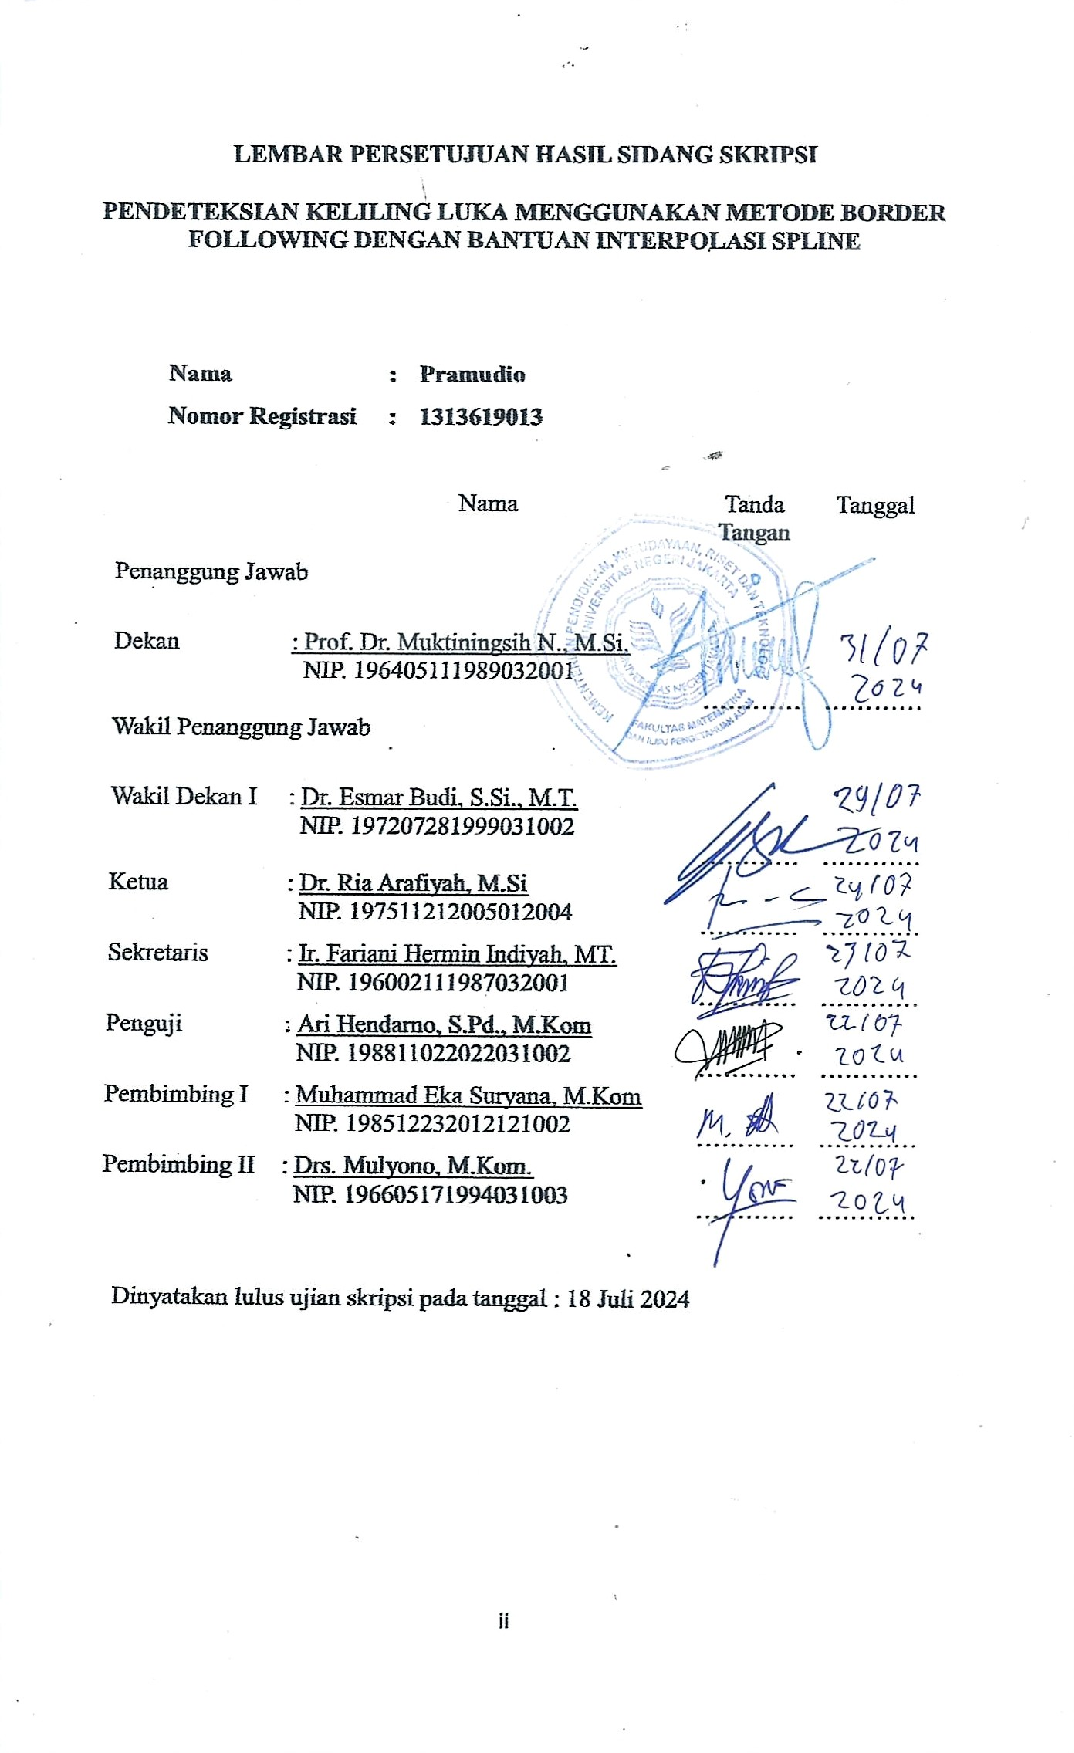
\includepdf[pages=-]{Lembar_Persetujuan.pdf}
\addcontentsline{toc}{chapter}{LEMBAR PERSETUJUAN}
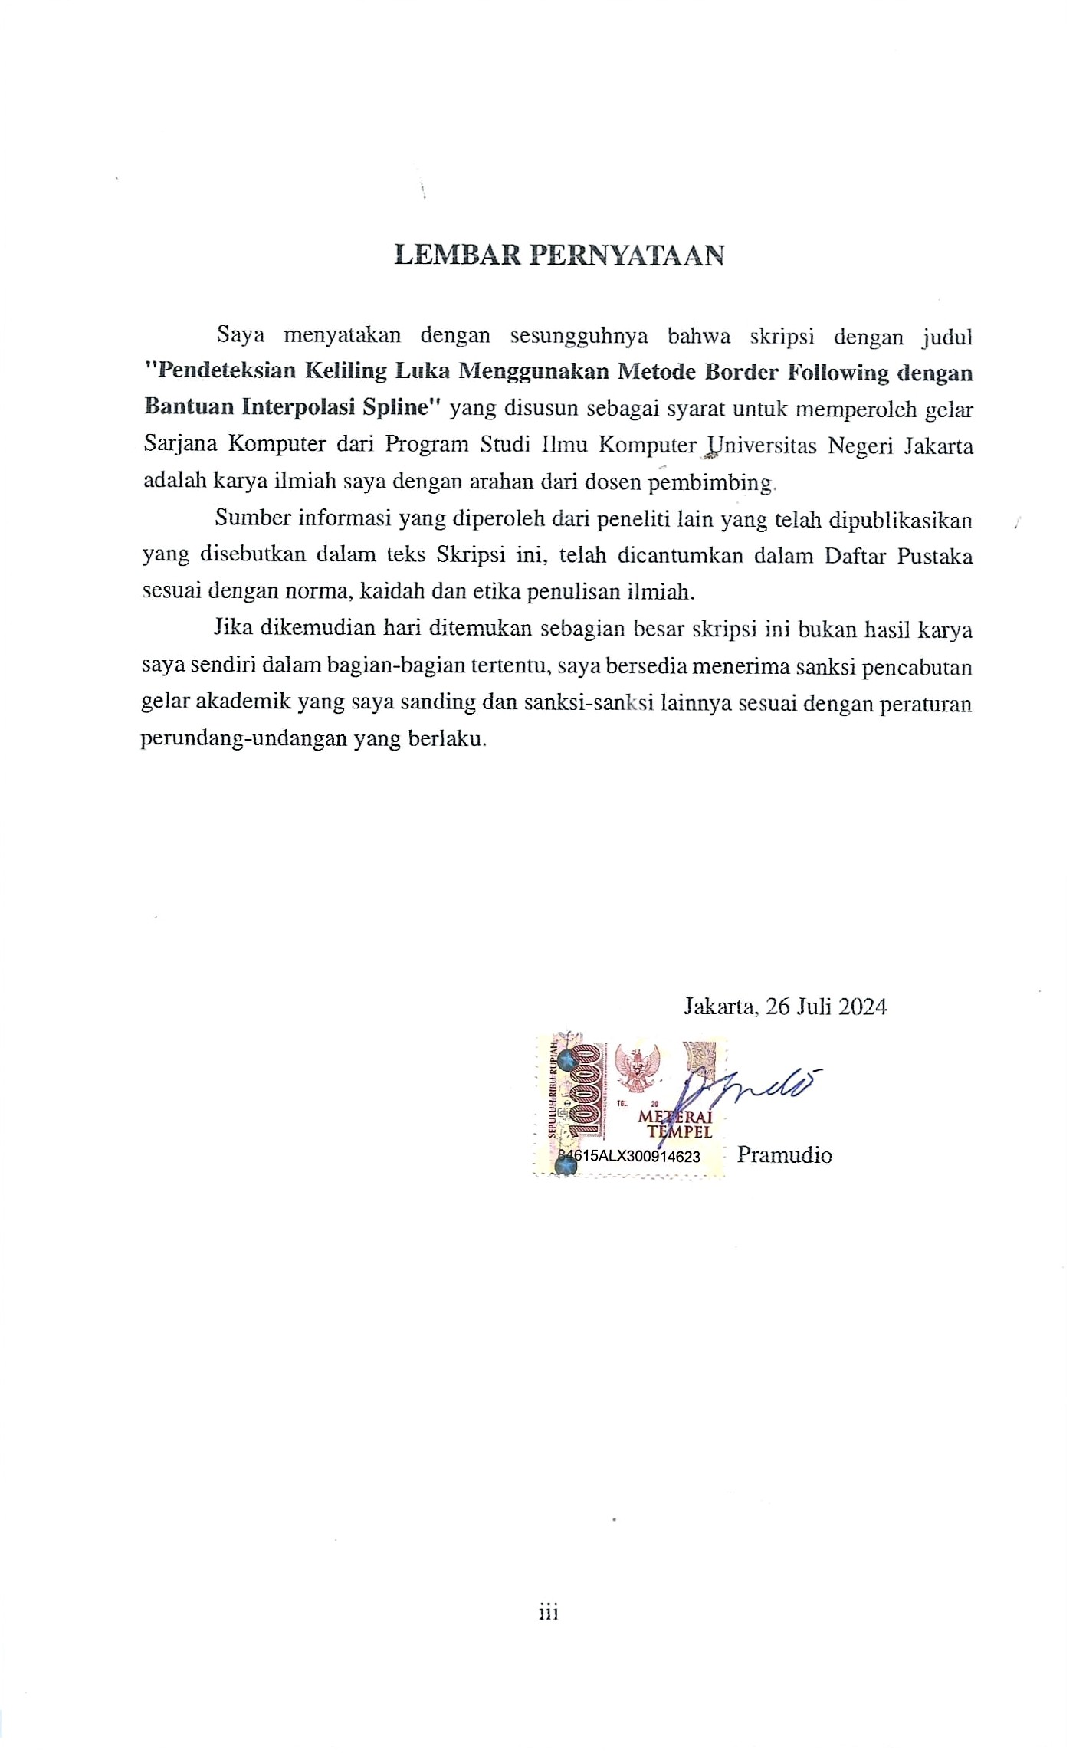
\includepdf[pages=-]{Lembar_Pernyataan.pdf}
\addcontentsline{toc}{chapter}{LEMBAR PERNYATAAN}
\chapter*{\centering{\large{KATA PENGANTAR}}}

Puji syukur atas kehadirat Allah Yang Maha Esa,
karena atas rahmat dan karunia-Nya yang melimpah 
penulis berhasil menyelesaikan 
skripsi ini dengan baik. Adapun jenis 
penelitian dengan judul 
\textit{Pendeteksian Keliling Luka Menggunakan Metode 
Border Following dengan Bantuan Interpolasi Spline}.

Dalam menyelesaikan skripsi ini, penulis selalu mendapat bantuan dari orang 
di sekitar penulis baik dalam bentuk bimbingan dalam mengerjakan skripsi 
ini maupun dorongan semangat dalam pengerjaan. Oleh maka dari itu, penulis 
ingin menyampaikan terima kasih yang sebesar-besarnya kepada:

\begin{enumerate}

	\item{Yth. Para petinggi di lingkungan FMIPA Universitas Negeri Jakarta}
	\item{Yth. Ibu Dr. Ria Arafiyah, M.Si selaku Koordinator Program Studi Ilmu
		Komputer.}
	\item{Yth. Bapak Muhammad Eka Suryana,M.Kom selaku Dosen Pembimbing I 
		yang telah membimbing dalam pengerjaan skripsi ini}
	\item{Yth. Bapak Drs. Mulyono, M.Kom selaku Dosen Pembimbing II yang telah
		membimbing dalam pengerjaan skripsi ini.}
	\item{Kedua orangtua penulis yang telah senantiasa mendukung,
	memberi semangat, serta mendoakan penulis}
	\item{Teman-teman yang telah memberikan dukungan dan bantuan dalam 
		pengerjaan skripsi ini.}
	
\end{enumerate}

Dalam penulisan skripsi ini penulis menyadari keterbatasan ilmu 
pengetahuan dan kemampuan penulis yang menyebabkan skripsi ini jauh dari 
sempurna, baik dari segi penulisan, penyajian materi, dan juga bahasa. Oleh 
karena itu penulis meminta kritik dan saran yang dapat dijadikan sebagai 
pembelajaran serta dapat membangun penulis agar lebih baik lagi dalam mengerjakan 
tugas-tugas dan permasalahan yang ada kedepannya.

Akhir kata, penulis berharap skripsi 
ini dapat bermanfaat bagi semua pihak baik itu 
bagi Ilmu Komputer Universitas Negeri Jakarta, teman-teman
serta para pembaca sekalian. Semoga Allah SWT 
senantiasa membalas kebaikan semua pihak yang 
telah membantu penulis dalam menyelesaikan skripsi ini.
\vspace{4cm}

\begin{tabular}{p{7.5cm}c}
	&Jakarta, 5 Juli 2024\\
	&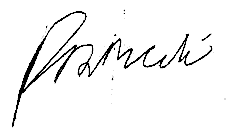
\includegraphics[keepaspectratio, width = 4cm]{gambar/TTD_Pramudio.png}\\
	&Pramudio
\end{tabular}

\backgroundsetup{
    scale=1,
    angle=0,
    opacity=0.25,
    contents={
        \begin{tikzpicture}[remember picture,overlay]
          \node at ([yshift = 0pt, xshift=0pt]current page.center)
            {
\includegraphics[scale = 0.75]{gambar/Logo-unj.png}};
        \end{tikzpicture}
    }
}
\chapter*{\centering{\large{ABSTRAK}}}
\singlespacing{}

\textbf{PRAMUDIO}, Pendeteksian Keliling Luka Menggunakan Metode  
\textit{Border Following} dengan Bantuan Interpolasi Spline. Skripsi, Program Studi Ilmu Komputer, Fakultas Matematika dan Ilmu Pengetahuan Alam, Universitas Negeri Jakarta. juli 2024.
\\
\\
Luka kronis merupakan salah satu penyakit yang kompleks, khususnya bagi penyandang
penyakit Diabetes Melitus (DM). Proses penyembuhan luka diawasi oleh pekerja medis 
dengan asesmen, yaitu mengukur keliling luka dan melihat warna luka. Setelah asesmen, 
pekerja medis baru bisa memberi keputusan dalam penanganan luka. 
Proses penyembuhan luka perlu melakukan asesmen 
yang tepat dan pengelolaan yang efektif, hanya saja asesmen manual dalam pengukuran 
luka sangat memakan waktu dan berpotensi mengganggu penyembuhan. Skripsi ini 
bertujuan untuk membantu pekerja medis dalam asesmen luka kronis penggunaan 
metode \emph{border following} dibantu dengan interpolasi \textit{spline} 
dalam pemrosesan citra untuk mengurangi asesmen luka manual. 
Penelitian ini memiliki potensi untuk memberikan analisis yang 
objektif dan reliabel dalam penggunaan pengolahan citra untuk 
asesmen luka kronis. Dengan memanfaatkan teknologi pengolahan citra, 
peneliti mencoba mengatasi keterbatasan metode asesmen 
luka manual dengan menggunakan algoritma \emph{border following}. 
Yang pertama dilakukan dalam metode ini adalah mengambil foto luka dengan 
menggunakan perangkat seluler, dilanjutkan dengan pemotongan citra untuk 
meningkatkan akurasi, lalu metode \textit{border following} dijalankan pada 
foto yang sudah dipotong untuk mendapatkan daerah kurva sekitar luka, selanjutnya 
dihaluskan menggunakan interpolasi \textit{spline}. Metode ini dilakukan pada 
ketiga kategori luka; merah, kuning, dan hitam yang sebanyak 69 data citra. Eksperimen 
ini menunjukkan \textit{border following} hanya dapat mendeteksi 14 luka dengan 
rata-rata akurasi masing-masing; merah 70.9$\%$ dengan 4 luka, kuning 73.4$\%$ 
pada 2 luka, dan hitam 92.6$\%$ pada 8 luka
\\
\\
\textbf{Kata kunci:} luka kronis, \textit{border following}, 
interpolasi \textit{spline}, asesmen luka, pemrosesan citra, asesmen luka, penyembuhan luka

\addcontentsline{toc}{chapter}{ABSTRAK}
\chapter*{\centering{\emph{\large{ABSTRACT}}}}
\singlespacing{}

\textbf{PRAMUDIO}, Detection of around Wound Perimeter Using the 
Border Following Algorithm with the Help of Spline Interpolation. Undergraduate Thesis, Computer Science Program, Faculty of 
Mathematics and Natural Sciences, State University of Jakarta. July 2024.
\\
\\
Chronic wounds one of complex illness, particularly for whose suffer 
Diabetes Mellitus (DM). The process of wound healing need to be monitored 
by medical worker with assessment, which measure area of wound and looking at 
the color of the wound. After the assessment, medical worker will make a decision 
for the wound treatment. 
The wound healing process involves appropriate assessment 
and effective management, yet manual methods in wound measurement often 
time-consuming and potentially interfere with healing. This thesis aims to 
help the medical worker to chronic wound assessment using the method of 
border following with the help of spline interpolation in image processing 
to lessen manual chronic wound assessment. This research holds the potential 
to bring analysis that are objective and reliable on the uses of image 
processing for chronic wound assessment. By utilizing technology of 
image processing, researcher tried to overcome the limitations of manual 
methods of chronic wound assessment with border following algorithm. 
The first to do with this method is to use phone to capture a photo, 
followed by croping the photo to increase accuracy, then border following 
method run on photo that are cropped to get curve area around the wound, 
next smoothed by using spline interpolation. This method used on three kind 
of wound; red, yellow and black with the quantity of 69 image data. This experiment 
bring forth border following can only detect 14 wound with the average of accuracy; 
red 70.9$\%$ with 4 wounds, yellow 73.4$\%$ from 2 wounds, and black 92.6$\%$ 
on 8 wounds.
\\
\\
\textbf{Keywords}: chronic wounds, border following, spline interpolation, 
image processing, wound assessment, wound healing.

\addcontentsline{toc}{chapter}{\textit{ABSTRACT}}
%\singlespacing{}
\tableofcontents{}
\addcontentsline{toc}{chapter}{DAFTAR ISI}
\listoffigures{}
\addcontentsline{toc}{chapter}{DAFTAR GAMBAR}
\listoftables{}
\addcontentsline{toc}{chapter}{DAFTAR TABEL}

\begin{counterpage}
\end{counterpage}
%Disini awal masukan untuk Bab
%-----------------------------------------------------------------
\onehalfspacing{}

%!TEX root = ./template-skripsi.tex
%-------------------------------------------------------------------------------
% 								BAB I
% 							LATAR BELAKANG
%-------------------------------------------------------------------------------

\chapter{PENDAHULUAN}

\section{Latar Belakang Masalah}

Kulit merupakan perlindungan pertama manusia dalam menjaga 
tubuhnya dari berbagai macam substansi. Apabila kulit 
terluka, maka diperlukan penanganan yang baik agar tidak 
terjadi infeksi.  Luka adalah keadaan di mana fungsi 
anatomis kulit normal mengalami kerusakan akibat proses 
patologis yang berasal dari internal maupun eksternal dan 
mengenai organ tertentu. Ketika luka tidak terinfeksi, 
maka pada normalnya luka tersebut akan melakukan 
penyembuhan. Proses penyembuhan terdapat beberapa fase, 
yaitu: hemostasis (beberapa jam pasca-terjadinya luka), 
inflamasi (1 - 3 hari), proliferasi (4 - 21 hari), dan 
remodelling (21 hari - 1 tahun). Fase-fase penyembuhan luka 
terjadi secara bertahap, namun dapat terjadi secara 
bersamaan (\textit{overlap}) (\cite{simon}).

Dari beberapa kondisi luka, terdapat luka yang proses 
penyembuhannya tidak normal dengan durasi fase-fase yang 
sesuai. Kondisi tersebut disebut dengan luka kronis 
(\cite{landen}), kondisi ini dapat memiliki kaitan dengan 
berbagai faktor yang memperlambat penyembuhan luka seperti 
adanya penyakit kronis, insufisiensi vaskuler, diabetes, 
gangguan nutrisi, penuaan, dan berbagai faktor lokal pada 
luka (tekanan, infeksi, dan edema). Secara umum, luka 
kronis dapat terjadi akibat ulkus vena, ulkus arteri, ulkus 
dekubitus, dan ulkus diabetik (\cite{zhao}).

Hal paling pertama yang dilakukan untuk menangani suatu 
masalah adalah mengidentifikasi masalah tersebut, luka 
tidak menjadi pengecualian. Pengidentifikasian luka yang 
akurat dapat membantu memberikan diagnosa yang akurat, 
penanganan luka yang tepat, memantau perbaikan luka, 
menghindari terjadinya komplikasi, serta dapat mengurangi 
biaya perawatan luka. Pengindentifikasian luka kronis 
umumnya didasarkan pada dua jenis tinjauan klinis, yaitu: 
tinjauan visual terhadap warna dominan luka dengan 
mengidentifikasi jaringan luka, dan tinjauan manual 
terhadap bentuk luka (area, perimeter, kedalaman, dan 
lain-lain) dengan pemeriksaan luka. Saat ini, tersedia 
dua teknik untuk pemeriksaan ini, yang pertama adalah 
metode manual langsung yang digunakan oleh dokter dan 
perawat untuk mengukur secara berkala dimensi luka 
menggunakan penggaris, dan teknik yang kedua adalah melacak 
batas luka pada kertas kalkir transparan yang ditempatkan 
pada kotak metrik. Kertas kalkir merupakan sebuah kertas 
yang memiliki permukaan yang tembus pandang dan sering 
digunakan oleh desainer untuk merancang desain atau gambar. 
Kertas ini memiliki struktur seperti kaca yang dapat 
dilihat secara tembus pandang ke bagian belakang kertas 
kalkir tersebut. Permukaan luka kemudian ditentukan dengan 
menghitung jumlah kotak secara manual setelah memindai 
gambar. Namun, kedua metode tersebut tidak dapat mengukur 
dimensi luka secara akurat dan kertas kalkir yang digunakan 
dapat menyebabkan infeksi pada luka (\cite{GuptaRTWS}). Salah 
satu metode yang diusulkan untuk mengatasi masalah ini 
adalah dengan menggunakan metode yang berbasis 
\textit{digital image processing}.

Metode berbasis \textit{digital image processing} merupakan 
alternatif untuk penilaian luka karena dapat memberikan 
langkah-langkah yang objektif, lebih akurat, dan dapat 
direproduksi. Salah satu keuntungan besarnya adalah metode 
ini memiliki resiko yang lebih rendah karena tidak ada kontak antara 
luka dan sistem pengukuran. Segmentasi citra merupakan 
proses mempartisi gambar digital menjadi beberapa segmen 
(set piksel, disebut juga \textit{superpixel}) yang 
memiliki fitur atau atribut yang sama. Segmentasi bertujuan 
untuk menyederhanakan atau mengubah representasi suatu 
citra menjadi sesuatu yang lebih bermakna dan lebih mudah 
untuk dianalisis. Segmentasi citra biasa digunakan untuk 
menemukan objek dan batas (seperti garis, kurva, dan 
lain-lain) dalam gambar (\cite{ShmmalaCBI}). Biasanya 
segmentasi menggunakan informasi lokal dalam gambar digital 
untuk menghitung segmentasi terbaik, seperti informasi 
warna yang digunakan untuk membuat histogram atau informasi 
yang mengindikasikan tepi, batas atau informasi tekstur 
(\cite{khattab}).

Segmentasi warna citra (\textit{color image segmentation}) 
didasarkan pada fitur warna piksel gambar yang 
mengasumsikan bahwa warna-warna homogen pada gambar 
bersesuaian dengan kelompok yang terpisah. Dengan kata 
lain, setiap kelompok mendefinisikan kelas piksel yang 
memiliki properti warna yang sama. Karena hasil segmentasi 
bergantung pada ruang warna (\textit{color space}) yang 
digunakan, tidak ada ruang warna tunggal yang dapat 
memberikan hasil yang dapat diterima untuk semua jenis 
gambar. Karena alasan ini, banyak penulis yang mencoba 
menentukan ruang warna yang sesuai dengan masalah 
segmentasi warna citra spesifik mereka (\cite{khattab}). 
Beberapa macam dari ruang warna (\textit{color space}), 
yaitu \textit{RGB, CMY(K), HSV, CIE, L*a*b, L*u*v,} dan 
\textit{YCrCb}. Setiap ruang warna (\textit{color space}) 
mempunyai sekurang-kurangnya 3 elemen warna dasar.

Salah satu cara mengidentifikasi luka adalah dengan 
tinjauan visual untuk identifikasi jaringan luka dari 
warna dominan. Warna luka akan memberikan banyak informasi 
penting berkaitan dengan perkiraan waktu penyembuhan luka, 
kondisi umum luka apakah dalam keadaan baik atau memburuk, 
dan risiko komplikasi. Warna tersebut dapat dipisahkan 
menjadi tiga warna, yaitu merah, kuning, dan hitam. 
Tinjauan visual ini, bisa dilakukan dengan metode 
segmentasi warna citra. Salah satu metode segmentasi warna 
citra yang telah dilakukan Aprilia Khairunnisa adalah 
dengan melihat ruang warna LAB terhadap segmentasi warna 
\textit{red, yellow, and black}. Proses segmentasi nya bisa 
dilakukan dengan menggunakan dua metode yaitu 
\textit{k-means} atau \textit{mean shift}. 
\textit{K-means} merupakan metode pengelompokan dari 
sejumlah \textit{cluster} yang terpisah. "K" mengacu pada 
jumlah \textit{cluster} yang ditentukan (\cite{YadavSeg}). 
Metode \textit{k-means} mempartisi \textit{n-set} input 
data menjadi \textit{k-cluster} di mana setiap set input 
data termasuk ke dalam cluster dengan mean terdekat 
(\cite{ZhengX}). Metode ini akan mempartisi data yang 
berkarakteristik sama ke dalam suatu kelompok yang sama dan 
data yang lainnya ke kelompok yang berbeda 
(\cite{Gustientiedina}). \textit{Mean shift} adalah teknik 
analisis \textit{non-parametic feature space} untuk mencari 
nilai maksimum dari fungsi kerapatan atau kepadatan yang 
diberikan dari data diskrit yang ada di fungsi tersebut. 
\textit{Mean shift} merupakan prosedur berulang (iteratif) 
sederhana yang menggeser setiap titik data ke rata-rata 
(\textit{mean}) titik data di daerahnya. Algoritma 
\textit{mean shift} disebut juga sebagai algoritma 
pencarian mode (\cite{ChengY}). 

Dari metode yang dilakukan oleh Aprilia Khairunnisa terdapat 
kekurangan, di mana hasil dari penelitiannya belum dapat 
memperlihatkan pengaruh dari penggunaan model warna LAB pada 
proses segmentasi (\cite{Aprilia}). ada satu hal yang masih 
dilakukan secara manual dalam proses metode tersebut, yaitu 
memasukkan hanya gambar luka saja, tanpa sekitar lukanya. 
Hal ini bisa dikembangkan dengan memasukan metode 
segmentasi yang mendeteksi tepi luka yaitu 
\textit{active contour}. 

Model \textit{active contour}, juga disebut \textit{Snake}, 
adalah \textit{framework} dalam pengolahan citra yang 
diperkenalkan oleh Michael Kass, Andrew Witkin, dan Demetri 
Terzopoulos untuk menggambarkan garis objek dari gambar 2D 
yang mungkin \textit{noisy}. Model \textit{active contour} 
populer dalam pengolahan citra, dan active contour banyak 
digunakan dalam aplikasi seperti \textit{object tracking}, 
\textit{shape recognition}, segmentasi, deteksi tepi, dan 
pencocokan stereo. \textit{Active contour} merupakan 
peminimalisir energi, dapat dideformasi yang terpengaruh 
oleh \textit{constraint} dan \textit{image forces} yang 
menarik ke arah objek kontur dan gaya di dalam yang menahan 
deformasi. \textit{Active contour} bisa diartikan sebagai 
model yang bisa dideformasi kepada citra dengan 
meminimalisir energi. Dalam dua dimensi, model bentuk aktif 
mewakili versi diskrit dari pendekatan ini, mengambil 
keuntungan dari model distribusi titik untuk membatasi 
rentang bentuk ke domain eksplisit yang dipelajari dari set 
pelatihan (\cite{kass}).

\emph{Active contour} merupakan metode yang biasanya tidak 
digunakan sendiri, dikarenakan metode ini perlu mengetahui 
bentuk suatu benda dan interaksi pengguna untuk mendapatkan 
hasil yang diinginkan. Pada Teknik yang dilakukan oleh 
Muhammad Rizki setelah memasukan citra dimulai dengan 
mengkonversi data \textit{RGB} menjadi \textit{grayscale}. 
Lalu gambar \textit{grayscale} tersebut mulai dideteksi 
menggunakan active contour di mana inisialisasi kurva 
awalnya yang seharusnya integer diubah dengan 
\textit{float}. Untuk rumusan energi internal, tidak diubah 
dari \textit{active contour} yang asli, tapi ketika masuk 
ke energi eksternal, persamaan yang dipakai berbeda sedikit. 
Setelah mendapatkan energi dari citra tersebut, dimulai 
proses update intersi kurva. Proses tersebut menggunakan 
memakai metode gradien arah direction untuk mendapatkan 
turunan pertama citra yang akan digunakan ke dalam rumus, 
lalu dilakukan iterasi yang dihitung melalui proses 
interpolasi (\cite{MRizki}).

Interpolasi dalam matematika umum adalah proses membuat 
suku-suku peralihan dari titik yang diketahui. Dalam 
pemrosesan gambar, biasanya digunakan untuk \textit{image scaling}, 
\textit{image resampling}, dan \textit{image resize}. Ada banyak algoritma 
yang saat ini digunakan untuk mengubah gambar digital. 
Kebanyakan dari mereka berupaya mereproduksi replika aslinya 
yang menarik secara visual. Sekarang seiring dengan 
teknologi untuk area tampilan yang lebih kecil untuk dilihat 
pada berbagai perangkat, ukuran gambar umumnya diambil 
sampelnya (atau disubsampel atau dikurangi) untuk 
menghasilkan thumbnail. Pengambilan sampel gambar 
(atau pembesaran atau interpolasi) paling umum dilakukan 
pada monitor atau televisi berukuran layar besar 
(\cite{Parsania}). Interpolasi yang akan dipakai penulis 
akan berdasarkan pada metode \textbf{NURBS} 
(\textit{Non-Uniform Rational B-Splines})(\cite{PiegTill96}) 
yang merupakan interpolasi penghalusan suatu kurva, ini 
bertujuan untuk menambahkan akurasi dalam pendeteksian luka, 
di mana pendeteksinya hanya menangkap tepi secara kasar.

seperti yang sudah tertuliskan dalam penilitian Muhammad 
Rizki, sebaiknya \textit{active contour} digantikan untuk 
meningkatkan akurasi deteksi luka (\cite{MRizki}). Dari metode 
yang dilakukan Muhammad Rizki, terdapat 
keunggulan di mana arah tepinya lebih jelas dibanding dengan 
citra asli sehingga membantu \textit{active contour} untuk 
melihat tepi suatu citra, tetapi ketika dilihat baik-baik, 
hasil dari gradien citra arah yang menggunakan interpolasi 
menambahkan arah tepi yang tidak diinginkan sehingga 
mengganggu pendeteksian \textit{active contour}. Untuk 
mengatasi masalah tersebut, penulis akan menggunakan 
algoritma \textit{Border Following} Suzuki.

Algoritma \textit{Border Following} 
suzuki merupakan salah satu algoritma topologi 
gambar biner digital yang pertama mendefinisikan hubungan 
hirarki antar pembatasan dan membedakan antara batas luar 
atau batas lubang.
Algoritma ini memindai gambar dari kiri ke kanan, mengecek 
ada nya objek piksel pada piksel yang dipindai. algoritma ini 
akan memindai sekitar piksel yang sedang dipindai untuk 
menentukan apakah piksel ini akan naik derajatnya. 
apabila sudah selesai pemindaian piksel ini, akan pindah 
pemindaian ke arah jarum jam, prioritas kanan. proses 
ini akan diulang sampai tidak ada piksel yang bisa digantikan
derajatnya. setelah sudah mendapatkan dari derajat dari 
semua piksel, maka bisa dilihat batas(\textit{border}) pada
gambar yang dipindai algoritma \textit{Border Following}(\cite{Suzuki}).

Penulis menginginkan untuk mengembangkan metode yang sudah 
pernah dilakukan oleh Muhammad Rizki(\cite{MRizki}). Penelitian ini 
bertujuan untuk meningkatkan akurasi dalam pendeteksian 
luka menggunakan \textit{active contour} dengan mengubah 
metode deteksi citra dengan \textit{border following}, lalu 
melakukan interpolasi pada hasil pendeteksian lukanya.
Penelitian ini bertujuan untuk membantu kalangan dokter dan 
perawat terkait penilaian luka kronis agar dapat memberikan 
hasil aproksimasi yang lebih dekat dengan \textit{ground
truth}(data asli yang diambil dari menggambar manual tepi luka).

\section{Rumusan Masalah}
Berdasarkan Latar belakang yang telah dikemukakan di atas, 
Fokus permasalahan pada penelitian ini adalah “Bagaimana 
mengembangkan pendeteksian keliling luka kronis menggunakan metode 
\textit{border following} yang dibantu dengan interpolasi spline”.

\section{Pembatasan Masalah}
Pembatasan masalah pada penelitian ini antara lain:
\begin{enumerate}
	\item Pendeteksian keliling luka kronis menggunakan 
	\textit{border following} yang dibantu dengan interpolasi 
	terhadap data citra luka yang 
	didapat dari penelitian luka Ns. Ratna Aryani, M.Kep, 
	tahun 2018 (\cite{Aryani:2018}).
	\item Penelitian dilakukan sampai mendapatkan hasil, 
	yaitu nilai akurasi dari selisih area kurva 
	\textit{border following} terhadap area 
	\textit{ground truth}(data asli yang diambil dari
	menggambar manual tepi luka).
\end{enumerate}

\section{Tujuan Penelitian}
Tujuan penelitian ini adalah untuk melanjutkan penelitian 
Rizki(\cite{MRizki}) dalam mendeteksi citra keliling luka dengan menggunakan metode 
\textit{Border Following} yang ditambahkan interpolasi spline
pada pendeteksi keliling luka kronis.

\section{Manfaat Penelitian}
\begin{enumerate}
	\item Bagi peneliti
		
	Penelitian ini merupakan media penerapan ilmu 
	pengetahuan, khususnya dalam pengembangan metode \textit{border following} 
	dalam pengkajian luka kronis serta membantu 
	penulis untuk menyelesaikan perkuliahan.
		
	\item Instansi Terkait
	 	
	Metode yang diajukan diharapkan dapat membuka peluang 
	untuk diajukan ke instansi kesehatan terkait dalam 
	proses pengkajian luka kronis.
	
	\item Bagi ilmu pengetahuan
	 	
	\begin{itemize}
		\item Mahasiswa
		
		Diharapkan penelitian ini dapat membantu dalam 
		penulisan paper yang bersangkutan dengan 
		pendeteksian luka.

		\item Bagi peneliti selanjutnya
		
		Diharapkan penelitian ini dapat dikembangkan oleh 
		peneliti selanjutnya untuk mengembangkan metode dari 
		penelitian ini.
	\end{itemize} 			
\end{enumerate}


% Baris ini digunakan untuk membantu dalam melakukan sitasi
% Karena diapit dengan comment, maka baris ini akan diabaikan
% oleh compiler LaTeX.
\begin{comment}
\bibliography{daftar-pustaka}
\end{comment}

 %!TEX root = ./template-skripsi.tex
%-------------------------------------------------------------------------------
%                            BAB II
%               KAJIAN TEORI
%-------------------------------------------------------------------------------

\chapter{KAJIAN PUSTAKA} 

\section{\emph{Border Following}}

Salah satu teknik yang sering dipakai dalam pengolahan citra 
adalah \textit{Border Following}, terutama citra biner. 
\textit{Border following} telah diteliti oleh beberapa orang 
karena taknik ini memiliki pengaplikasian yang cukup luas, 
seperti pengenalan objek, analisis citra, deteksi objek, dan 
kompresi data citra (\cite{Suzuki})

Dalam penelitian yang dibuat oleh Suzuki, ia menawarkan 
dua algoritma \textit{border following} yang sampai saat ini 
masih digunakan oleh \textit{library} pengolahan citra yang 
umum diketahui yaitu \textbf{OpenCV}. Algoritma ini merupakan 
salah satu algoritma yang mengenalkan pendefinisian hubungan 
hierarki antar tepi (\textit{border}). Tidak hanya itu, 
algoritma ini juga membedakan tepi lubang (\textit{hole}) 
dan tepi luar (\textit{outer border}) di sebuah objek. 
Suzuki memberikan definisi pada algoritma ini, yaitu:
\begin{itemize}
	\item \textbf{Definisi 1 (\textit{border point})}.
	Sebuah piksel bernilai 1 yang dikelilingi oleh piksel
	bernilai 0 dapat disebut sebagai \textit{border point}.

	\item \textbf{Definisi 2 (komponen yang mengelilingi
	komponen lain.)}. Dari gambar 
	(\ref{gambar:Keliling_antar_komponen}) dapat dikatakan 
	bahwa komponen $S_2$ mengelilingi komponen $S_4$

	\item \textbf{Definisi 3(\textit{outer border} dan \textit{hole border})}. 
	Sebuah rangkaian \textit{border point} antar komponen yang 
	mempunyai nilai piksel 1 (objek) dengan komponen yang 
	mempunyai nilai piksel 0 (latar belakang)

	\item \textbf{Definisi 4(\textit{parent border})}. 
	Berdasarkan gambar (\ref{gambar:Keliling_antar_komponen}) 
	dapat dikatakan bahwa tepi $B_2$ adalah 
	\textit{parent border} dari tepi $B_3$

	\item \textbf{Definisi 5(tepian yang mengelilingi tepian 
	lain)}. Dari gambar (\ref{gambar:Keliling_antar_komponen}) 
	dapat dikatakan bahwa tepi $B_2$ mengelilingi tepi $B_3$.
\end{itemize}

\begin{figure}[H]
	\centering
	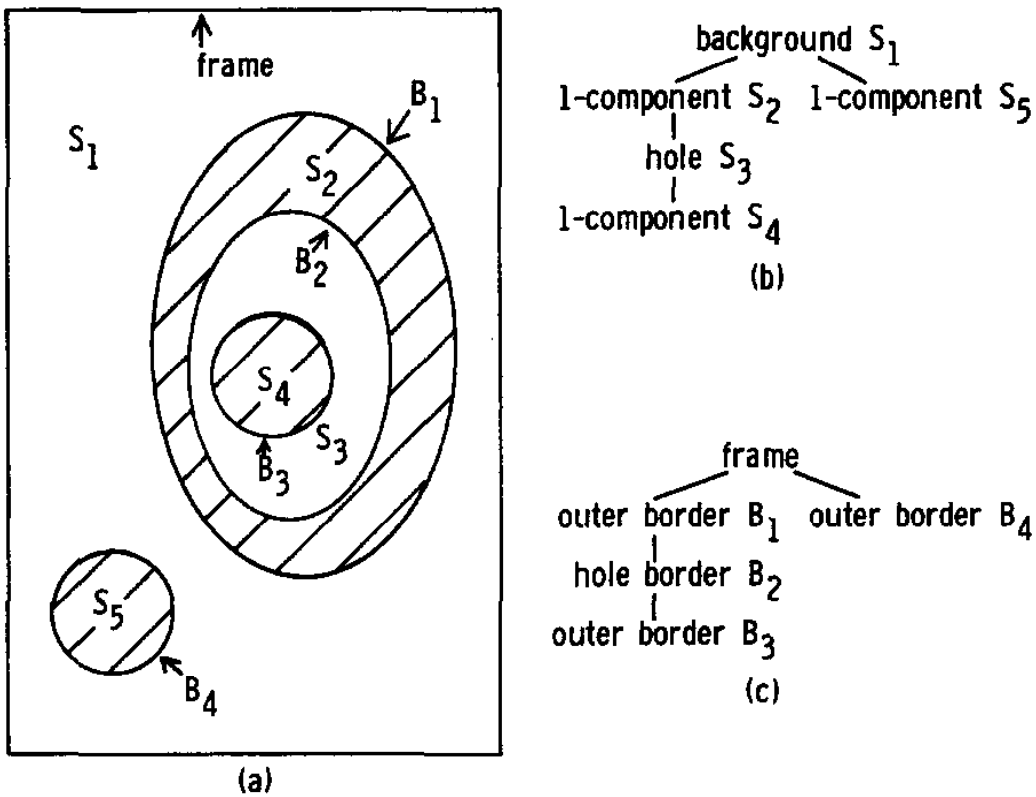
\includegraphics[keepaspectratio, width=10cm]{gambar/BorderFollowingPustaka/pic1.png}
	\caption{\textit{surroundness} antar komponen yang terhubung (b) 
	dan antar tepi(\textit{borders}) (c).}
	\label{gambar:Keliling_antar_komponen}
\end{figure}

Diasumsikan citra yang dimasukan algoritma ini 
berupa citra biner. Piksel dengan nilai 0 dan 1 
disebut sebagai 0-piksel dan 1-piksel. Nilai sebuah 
piksel dalam koordinat ($i,j$) yang masing-masing 
melambangkan baris dan kolom sebuah citra digital 
didefinisikan sebagai $f_{i,j}$. Baris paling pinggir
yang berada di atas, kanan, bawah, dan kiri adalah 
\textit{frame}(bingkai) dari citra tersebut. Dalam hal
ini, setiap tepi baru yang ditemukan akan diberi angka 
unik dan disebut sebagai \textbf{NBD}. Asumsikan NBD dari
\textit{frame} adalah 1, sementara tepi lain diberi angka 
NBD secara berurutan. Nilai NBD dari \textit{parent} 
setiap tepi di dalam variabel \textbf{LNBD} kemudian 
disimpan. Berikut merupakan langkah-langkah 
algoritma pertama \textit{border following}:

Dimulai dengan pemindaian piksel citra dari kiri ke kanan
hingga \textit{scanner} menemukan piksel objek 
($f_{i,j} \neq 0$). Dilanjutkan dengan menentukan 
apakah piksel tersebut merupakan tepi luar atau tepi 
lubang. Untuk setiap baris baru yang dipindai, 
kembalikan nilai LNBD ke 1.

\begin{enumerate}
	\item Langkah 1
	\begin{enumerate}[(a)]
		\item jika $f_{i,j} = 1$ dan $f_{i,j-1} = 0$, 
		maka piksel ($i,j$) adalah \textit{starting 
		point} dari operasi \textit{border following} 
		untuk tepi luar(\textit{outer border}). 
		inkremen NBD dan set ($i_2, j_2$) $\gets$ ($i, j-1$).
		\item jika $f_{i,j} \geq 1$ dan $f_{i,j+1} = 0$, 
		maka piksel ($i,j$) adalah \textit{starting 
		point} dari operasi \textit{border following} 
		untuk tepi lubang(\textit{hole border}). 
		inkremen NBD, set ($i_2, j_2$) $\gets$ ($i, j+1$), 
		dan LNBD $\gets f_{i,j}$ jika $f_{i,j} > 1$
		\item jika kedua kondisi tidak terpenuhi, maka
		lanjut ke langkah 4.
		\begin{figure}[H]
			\centering
			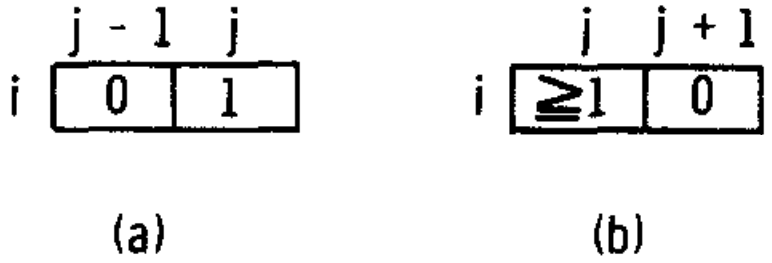
\includegraphics[keepaspectratio, width=6cm]{gambar/BorderFollowingPustaka/pic2.png}
			\caption{kondisi \textit{starting point} 
			dari algoritma \textit{border following} 
			untuk tepi luar (a) dan tepi lubang (b)}
			\label{gambar:kondisi_batas}
		\end{figure}
	\end{enumerate}
	\item Langkah 2 \\
	Tentukan \textit{parent border} untuk tepi piksel ($i,j$) 
	berdasarkan jenis tepi piksel dari piksel ($i,j$) dan LNBD
	(tepi terakhir yang ditemukan), mengikuti aturan pada tabel 
	(\ref{tabel:aturan_parent})
	\begin{table}[H]
		\caption{Aturan penetapan \textit{parent border}}
		\begin{tabular}[width=6cm]{| c | c | c |}
			\hline
			& \multicolumn{2}{|c|}
			{\textit{Type of border B' with the 
			sequentioal number of LNBD}} \\
			\hline
			\textit{Type of B} & \textit{Outer border} 
			& \textit{Hole border} \\
			\hline
			\textit{Outer border} & \textit{The parent border 
			of the border B'} & \textit{The border B'} \\
			\textit{Hole border} & \textit{The border B'} 
			&\textit{The parent border of the border B'} \\
			\hline
		\end{tabular}
		\label{tabel:aturan_parent}
	\end{table}
	\item langkah 3 \\
	Proses \textit{border following} dimulai dari 
	\textit{starting point} piksel ($i,j$) pada langkah ini
	\begin{enumerate}[(a)]
		\item Dimulai dari piksel ($i_2,j_2$), periksa piksel
		tetangga searah jarum jam dari piksel ($i,j$) sampai
		menemukan piksel \textit{non-zero}. Piksel \textit{non-zero}
		yang pertama ditemukan didefinisikan sebagai 
		($i_1,j_1$). jika piksel \textit{non-zero} tidak 
		ditemukan, set $f_{i,j} =$ -NBD dan lanjutkan ke langkah
		keempat
		\item $(i_2,j_2) \gets (i_1,j_1)$ dan
		$(i_3,j_3) \gets (i,j)$
		\item Mulai dari elemen setelah piksel($i_2,j_2$), mencari
		piksel \textit{non-zero} di sekitar piksel ($i_3,j_3$) 
		dengan arah berlawanan jarum jam dan set piksel 
		\textit{non-zero} pertama yang ditemukan ke dalam
		variabel ($i_4,j_4$).
		\item Ubah nilai $f_{i_3,j_3}$ dari piksel ($i_3,j_3$) 
		dengan aturan menandai(\textit{marking policy}):
		\begin{enumerate}[i]
			\item Jika piksel ($i_3,j_3+1$) 
			adalah 0-piksel (piksel bernilai 0), set
			$(i_3,j_3+1) \gets$ -NBD
			\item Jika piksel ($i_3,j_3+1$)  
			bukan 0-piksel (piksel bernilai 0), set
			$(i_3,j_3+1) \gets$ NBD
			\item Jika kedua kondisi di atas tidak terpenuhi,
			jangan ubah nilai $f_{i_3,j_3}$
		\end{enumerate}
		\item Jika $(i_4,j_4) = (i,j)$ dan $(i_3,j_3) = (i_1,j_1)$
		(kembali ke \textit{starting point}), maka lanjut ke 
		langkah 4, jika tidak set $(i_2,j_2) \gets (i_3,j_3)$, 
		$(i_3,j_3) \gets (i_4,j_4)$ dan kembali ke langkah (3.c).
	\end{enumerate}
	\item Langkah 4 \\
	jika $f_{i,j} \neq 1$, maka LNBD $\gets |f_{i,j}|$ dan
	lanjutkan pemindaian dari mulai piksel ($i,j+1$) 
	untuk kembali mencari nilai piksel objek $f_{i,j} \neq 0$.
	Algoritma dinyatakan selesai jika pemindai sudah sampai
	sudut kanan bawah dari citra(piksel terakhir)
\end{enumerate}
\begin{figure}[H]
	\centering
	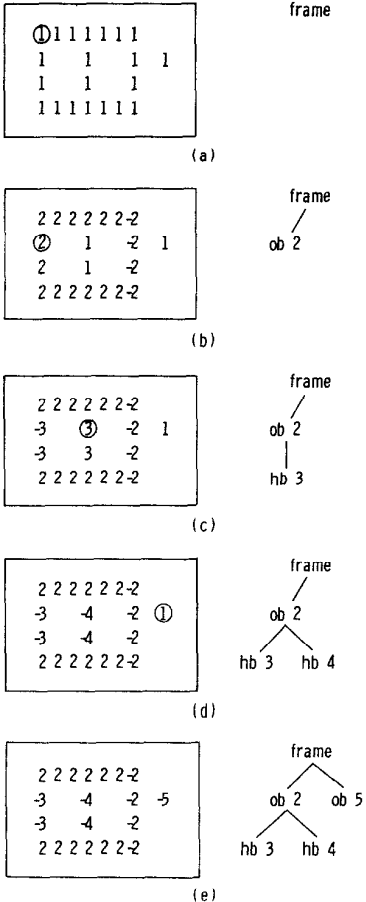
\includegraphics[keepaspectratio, width=7cm]{gambar/BorderFollowingPustaka/pic3.png}
	\caption{Ilustrasi proses pemberian hierarki terhadap piksel citra; 
	lingkaran pada piksel menunjukkan titik mula pindai \textit{border following}}
	\label{gambar:ProsesJalanBorderFollowing}
\end{figure}

\begin{figure}[H]
	\centering
	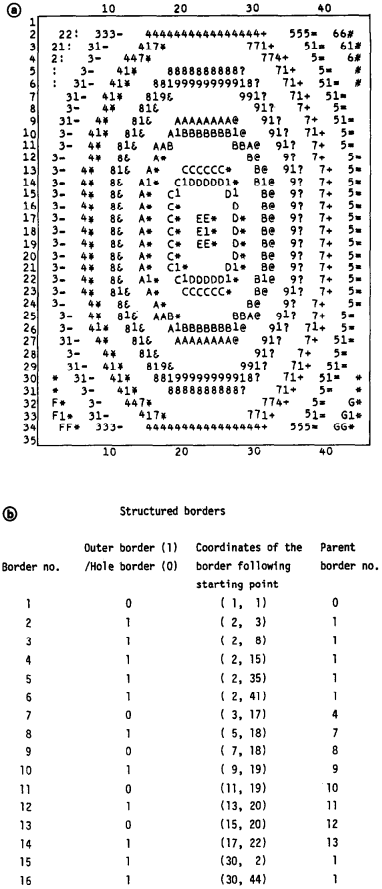
\includegraphics[keepaspectratio, width=9cm]{gambar/BorderFollowingPustaka/pic4.png}
	\caption{Struktur topologi antara tepi satu 
	dengan tepi yang lain jika menggunakan Algoritma 
	pertama. Hasil citra (a) dan Struktur yang diekstrak (b)}
	\label{gambar:Analisis_struktur_topologi}
\end{figure}

Selain algoritma pertama Suzuki, ia juga mengusulkan algoritma
kedua \textit{border following} di mana hasilnya hanya tepi 
terluarnya saja.Berikut perbedaan algoritma pertama dan 
algoritma kedua yang diusulkan Suzuki:
\begin{enumerate}
	\item Kondisi \textit{starting point} untuk melakukan
	operasi \textit{border following} hanya berlaku
	untuk tepi terluar (gambar \ref{gambar:kondisi_batas}) 
	dan jika LNBD $\leq 0$.
	\item \textit{Marking policy} tetap sama dengan algoritma
	pertama (langkah 3.d), tetapi nilai NBD dan -NBD akan
	diganti masing-masing dengan nilai 2 dan -2
	\item Nilai LNBD juga tetap disimpan dari piksel 
	\textit{non-zero} yang ditemukan sebelumnya. Akan
	tetapi, LNBD akan di-\textit{reset} ke nilai 0
	untuk setiap bari baru yang dipindai
\end{enumerate}

\begin{figure}[H]
	\centering
	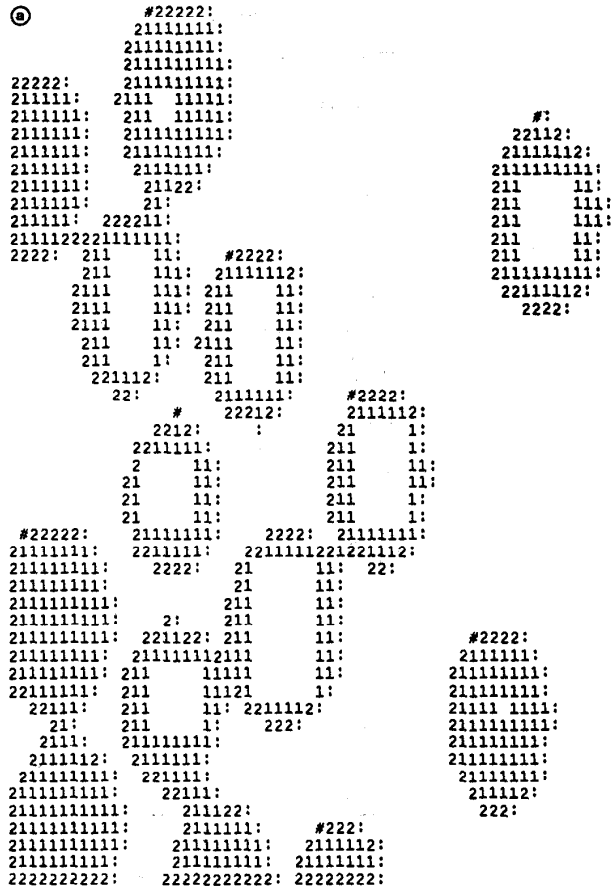
\includegraphics[keepaspectratio, width=8cm]{gambar/BorderFollowingPustaka/pic5.png}
	\caption{Hasil penciutan blob dengan 
	Algoritma kedua. “\#” merepresentasikan 
	\textit{starting point} dari tepi terluar, 
	“:” menunjukkan nilai -2.}
	\label{gambar:hasil_penciutan_blob}
\end{figure}

\section{\emph{Splines interpolation imaging}}

Pada konteks pengolahan citra, Interpolasi merupakan proses 
pembangunan kurva atau \textit{spline}, atau permukaan(\textit{surface}) terdefinisi 
bebas yang melalui sekumpulan titik data(\textit{data points}) 
secara tepat. Terkadang diberikan pembatas tambahan untuk 
mendapatkan interpolasi yang dibatasi agar mendapatkan hasil 
kurva atau \textit{spline} yang diinginkan(\cite{lockyer2006controlling}). \textit{Spline} 
yang sering dirujuk pada pengolahan citra adalah kurva yang 
dibentuk dengan gabungan polinominal. Contoh \textit{Spline} 
yang sudah di-interpolasikan dapat dilihat pada gambar (\ref{gambar:contohchordlength})


\subsection{\emph{Bézier Spline}}

Bézier \textit{Spline} merupakan salah satu kurva polinominal 
menggunakan kumpulan diskrit titik kontrol untuk 
membuat kurva yang halus dan kontinu. 

Bézier \textit{spline} dengan derajat ke-$n$ terdefinisikan 
sebagai berikut
\begin{equation}
	\begin{split}
		\textbf{C}(u) = \sum_{i = 0}^{n} B_{i,n}(u) \textbf{P}_i \quad
		& 0 \leq u \leq 1
	\end{split}
	\label{kurvabezier}
\end{equation}
Fungsi dasar (\textit{blending}), $\{B_{i,n}(u)\}$, merupakan 
polinominal Bernstein yang didefinisikan sebagai
\begin{equation}
	B_{i,n}(u) = \frac{n!}{i!(n-i)!} u^i (1-u)^{n-1}
	\label{bernstein}
\end{equation}
Koefisien geometri dalam bentuk ini, $\{\textbf{P}_i\}$, disebut 
sebagai titik kontrol(\textit{control points}), dan pada 
persamaan (\ref{kurvabezier}), $u$ nya harus diantara 0 sampai 1 
$[u \in [0,1]]$

Bisa dicontohkan hasil Bézier sebagai berikut. Bézier 
memiliki derajat 2, $n = 2$, tarik dari persamaan 
(\ref{kurvabezier}) dan (\ref{bernstein}), bisa didapat
$\textbf{C}(u) = (1 - u)^2 \textbf{P}_0 + 2u(1 - u) 
\textbf{P}_1 + u^2 \textbf{P}2$ akan menghasilkan 
busur parabola dari $\textbf{P}_0$ ke $\textbf{P}_2$. 
Dapat kita lihat pada gambar(\ref{gambar:Bezier_derajat2})
\begin{itemize}
	\item poligon yang dibentuk oleh 
	$\{\textbf{P}_0, \textbf{P}_1, \textbf{P}_2\}$, 
	disebut sebagai \textit{control polygon}, mendekati 
	bentuk kurva yang cukup baik.
	\item $\textbf{P}_0 = \textbf{C}(0)$ dan 
	$\textbf{P}_2 = \textbf{C}(1)$.
	\item arah tangen kepada kurva yang berada di titik akhir 
	paralel terhadap $\textbf{P}_1 - \textbf{P}_0$ dan 
	$\textbf{P}_2 - \textbf{P}_1$.
	\item kurva berada di dalam segitiga yang dibentuk 
	$\textbf{P}_0\textbf{P}_1\textbf{P}_2$
\end{itemize}
\begin{figure}[H]
	\centering
	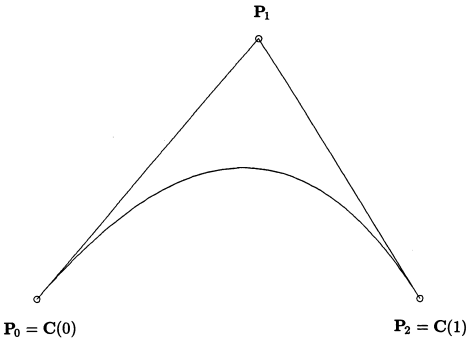
\includegraphics[keepaspectratio, width=10cm]{gambar/Interpolasi/bezierderajat2.png} 
	\caption{Kurva Bézier berderajat-2.}
	\label{gambar:Bezier_derajat2}
\end{figure}


\subsection{\emph{B-Spline}}

pada analisis numerik dalam matematika, 
\textit{B-Spline} atau bisa disebut dengan 
\textit{basis spline} merupakan fungsi spline dengan 
tunjangan yang sedikit dengan diberikan derajat, kehalusan, 
dan partisi domain.
Kurva yang hanya berisikan satu polinomial atau 
segmentasi rasional yang sering tidak memadai, 
kekurangannya adalah:
\begin{itemize}
	\item memerlukan \textit{high degree}(interpolasi 
	dengan derajat tinggi) untuk kompensasi  
	banyak keterbatasan; misalnya, ($n - 1$)-derajat 
	diperlukan untuk melewatkan kurva Bézier polinomial 
	melalui $n$ titik data. Namun, kurva tingkat tinggi 
	tidak efisien untuk diproses dan secara numerik tidak stabil;
	\item Suatu \textit{high degree} diperlukan untuk 
	\textit{fitting} bentuk(formula) kompleks secara akurat
	\item kurva segment tunggal (\textit{surface} atau 
	disebut permukaan) tidak cocok untuk desain 
	bentuk(formula) interaktif; meskipun kurva Bézier dapat 
	dibentuk melalui titik kontrolnya (dan bobot), 
	kontrolnya tidak cukup lokal.
\end{itemize}

Solusinya adalah dengan menggunakan kurva (atau permukaan) 
yang \textit{piecewise polynomial}(polinomial yang dipotong-potong), 
atau \textit{piecewise rational}(rasional yang dipotong-potong). 
Gambar (\ref{gambar:Kurva_dipotong_tiga}) 
menunjukkan kurva $\textbf{C}(u)$, yang terdiri 
dari $m$ (= 3) segmen polinomial  berderajat-$n$. 
$\textbf{C}(u)$ didefinisikan pada $u\in$ [0, 1]. 
Nilai parameter $u_0 = 0 < u_1 < u_2 < u_3$ = 1 disebut 
\textit{breakpoints}. Mereka memetakan ke titik akhir dari 
tiga segmen polinomial. ditunjukkan segmen 
sebagai $\textbf{C}_{i}(u)$, $1 \leq i \leq m$. 
Segmen-segmen tersebut 
dibangun sedemikian rupa sehingga bergabung dengan 
tingkat kontinuitas tertentu (tidak harus sama di 
setiap \textit{breakpoint}). Misalkan 
$\textbf{C}_{i}^{(j)}$ menyatakan 
turunan ke-$j$ dari $\textbf{C}_i$. $\textbf{C}(u)$ 
dikatakan $\textbf{C}^k$ kontinu pada \textit{breakpoint} 
$u_i$ jika $\textbf{C}_{i}^{(j)}(u_i) = C_{i+1}^{(j)}(u_i)$ 
untuk semua $0 \leq j \leq k$.
\begin{figure}[H]
	\centering
	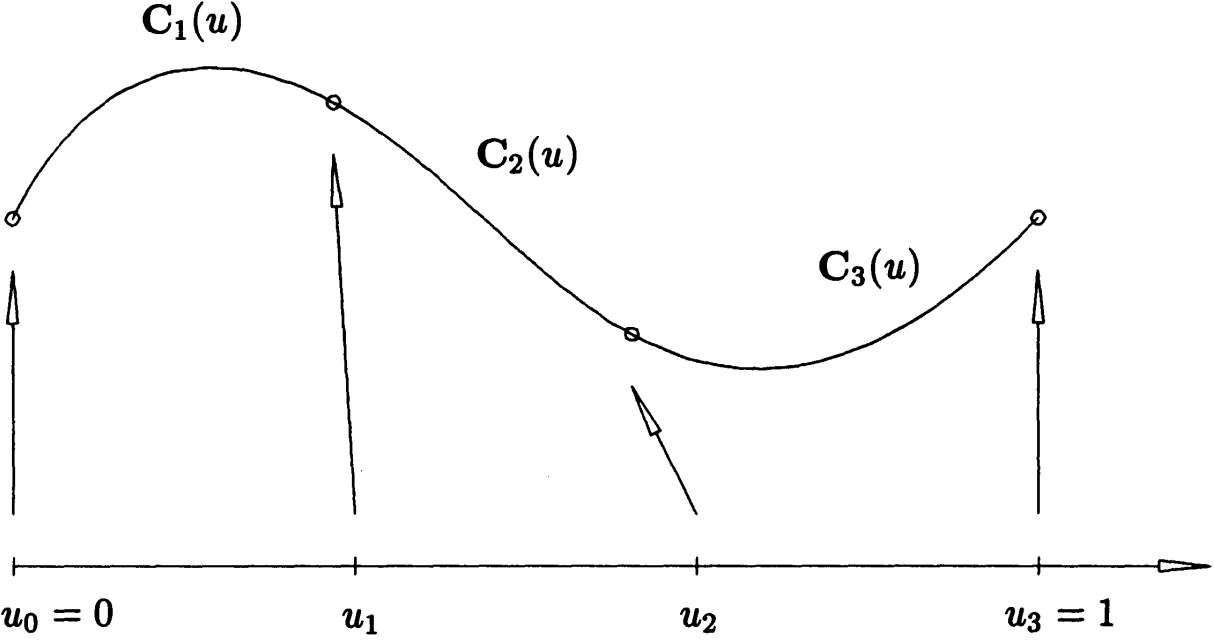
\includegraphics[keepaspectratio, width=10cm]{gambar/Interpolasi/pic1.png} 
	\caption{Kurva polinomial kubik dipotong tiga segmen.}
	\label{gambar:Kurva_dipotong_tiga}
\end{figure}

Setiap bentuk polinomial standar dapat digunakan 
untuk menyatakan bentuk $\textbf{C}_{i}(u)$. 
Gambar (\ref{gambar:Kurva_dipotong_tiga_dipotong_lagi}) 
menunjukkan kurva Gambar (\ref{gambar:Kurva_dipotong_tiga}) 
dengan tiga segmen  dalam bentuk kubik Bézier. 
$\textbf{P}_i^j$ menunjukkan titik kontrol ke-$i$ dari segmen ke-$j$.
\begin{figure}[H]
	\centering
	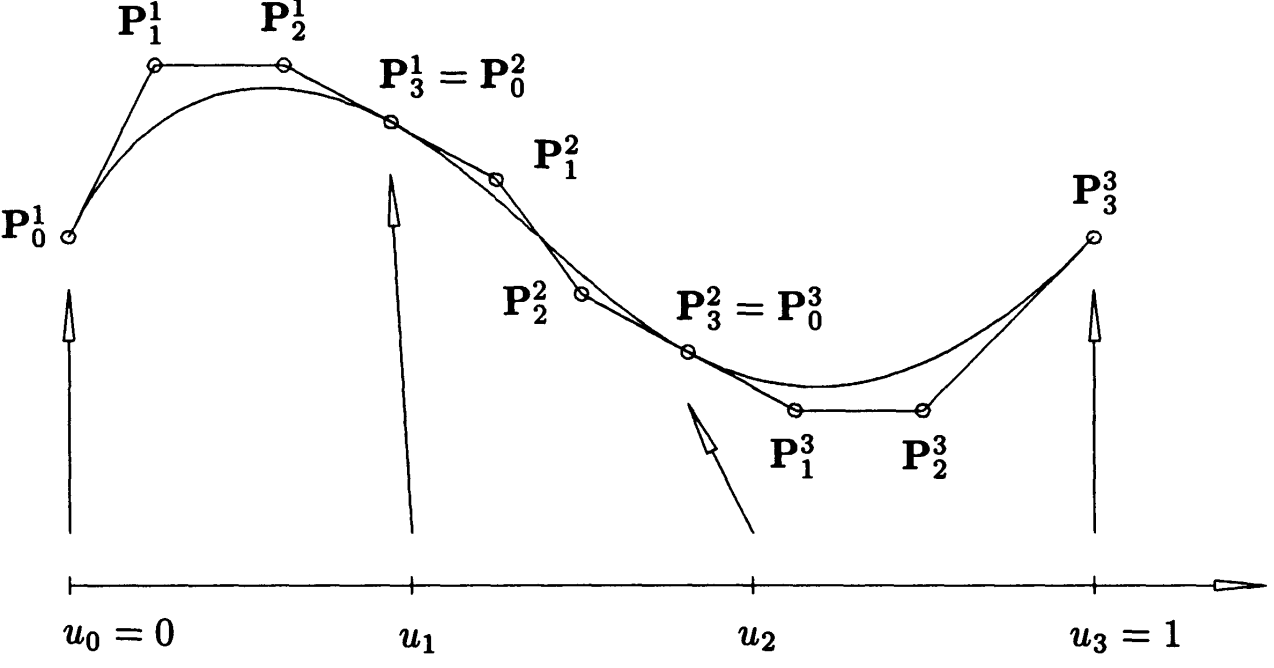
\includegraphics[keepaspectratio, width=10cm]{gambar/Interpolasi/pic2.png} 
	\caption{Kurva Gambar (\ref{gambar:Kurva_dipotong_tiga}) 
	ditunjukkan dengan segmen polinomial yang direpresentasikan 
	dalam bentuk Bézier.}
	\label{gambar:Kurva_dipotong_tiga_dipotong_lagi}
\end{figure}

Jika derajatnya sama dengan tiga dan \textit{breakpoints} 
$U = {u_0, u_1, u_2, u_3}$ tetap, dan jika dua 
belas titik kontrol, $\textbf{P}_i^j $, bervariasi 
secara sembarangan, akan memperoleh ruang vektor, $\nu$, 
yang terdiri dari semua potongan kurva polinomial 
kubik di $U$. $\nu$ memiliki dimensi dua belas, dan kurva 
di $\nu$ mungkin terputus-putus di $u_1$ atau $u_2$. 
Sekarang misalkan ditetapkan (seperti pada 
Gambar (\ref{gambar:Kurva_dipotong_tiga_dipotong_lagi})) 
bahwa $\textbf{P}_3^1 = \textbf{P}_0^2$ 
dan $\textbf{P}_3^2 = \textbf{P}_0^3$. Hal ini 
akan menghasilkan $\nu^0$, ruang vektor dari semua 
potongan kurva polinomial kubik pada $U$ yang 
setidaknya $\textbf{C}^0$ kontinu di semua titik. $\nu^0$ memiliki 
dimensi sepuluh, dan $\nu^0 \subset \nu$

Dari paragraf di atas, bisa dibuat kurva yang 
representatif dalam bentuk:

\begin{equation}
	\textbf{C}(u) = \sum_{i = 0}^{n} f_{i}(u) \textbf{P}_i
	\label{rumusdasarB}
\end{equation}
\begin{itemize}
	\item $\textbf{P}_i$ adalah titik kontrol
	\item {$f_{i}(u), i = 0$, ..., $n$} adalah 
	potongan fungsi polinomial yang membentuk 
	basis untuk ruang vektor semua fungsi potongan 
	polinomial dengan derajat dan kontinuitas yang 
	diinginkan (untuk sebuah urutan breakpoint tetap, 
	$U = {u_i}$, $0 \leq i \leq m$)
\end{itemize}
Perhatikan bahwa kontinuitas ditentukan oleh 
fungsi basis\textit{basis function}, sehingga 
titik kontrol dapat dimodifikasi tanpa mengubah 
kontinuitas kurva. Selain itu, {$f_i$} harus memiliki 
sifat analitik bagus yang 'biasa'. Hal ini 
memastikan bahwa kurva yang ditentukan oleh 
Persamaan (\ref{rumusdasarB}) memiliki sifat 
geometri yang mirip dengan kurva Bézier, misalnya 
\textit{convex hull}, \textit{variation diminishing}, 
\textit{transformation invariance}. Properti penting 
lainnya yang dicari dalam fungsi basis ini adalah \textit{local support}; 
ini menyiratkan bahwa setiap $f_{i}(u)$ bukan nol 
hanya pada sejumlah subinterval yang terbatas, 
bukan seluruh domain, [$u_0$, $u_m$]. Karena $\textbf{P}_i$ 
dikalikan dengan $f_{i}(u)$, pergerakan $\textbf{P}_i$ 
mempengaruhi bentuk kurva hanya pada subinterval 
di mana $f_{i}(u)$ bukan nol.

Ada banyak cara untuk mendefinisikan $f_{i}(u)$ 
pada rumus (\ref{rumusdasarB}), di sini akan memakai 
cara \textit{recurrence formula}. Misalkan $U = {u_0, \dots, um}$ 
adalah barisan bilangan real tak menurun, yaitu 
$u_i \leq u_i+1$, $i = 0, \dots, m - 1$. $u_i$ disebut 
\textit{knots}, dan $U$ adalah \textit{knots vector}. 
Fungsi basis \textit{B-spline} ke-$i$ merupakan $p$-derajat 
(ordo $p+l$), dilambangkan dengan $N_{i,p}(u)$, 
didefinisikan sebagai
\begin{equation}
	\begin{split}
	&N_{i,0}(u) = \begin{cases}
		1 \quad \text{if} \quad u_i \leq u < u_{i+1} \\
		0 \quad \text{otherwise}
	\end{cases}
	\\
	&N_{i,p}(u) = \frac{u - u_i}{u_{i+p} - u_i}N_{i,p-1}(u) + \frac{u_{i+p+1} - u}{u_{i+p+1} - u_{i+1}}N_{i+1,p-1}(u)
	\label{rumusdasarN}
	\end{split}
\end{equation}
Dengan catatan :
\begin{itemize}
	\item $N_{i,0}(u)$ merupakan fungsi langkah(\textit{step function})
	yang hampir semua hasilnya merupakan nol kecuali 
	di dalam interval setengah terbuka $u \in [ui, u{i+1})$
	\item Untuk $p > 0, N_{i,p}(u)$ merupakan kombinasi 
	linear dari dua fungsi dasar ($p$ - 1)-derajat. 
	(gambar \ref{gambar:definisirumusdasar})
	\begin{figure}[H]
		\centering
		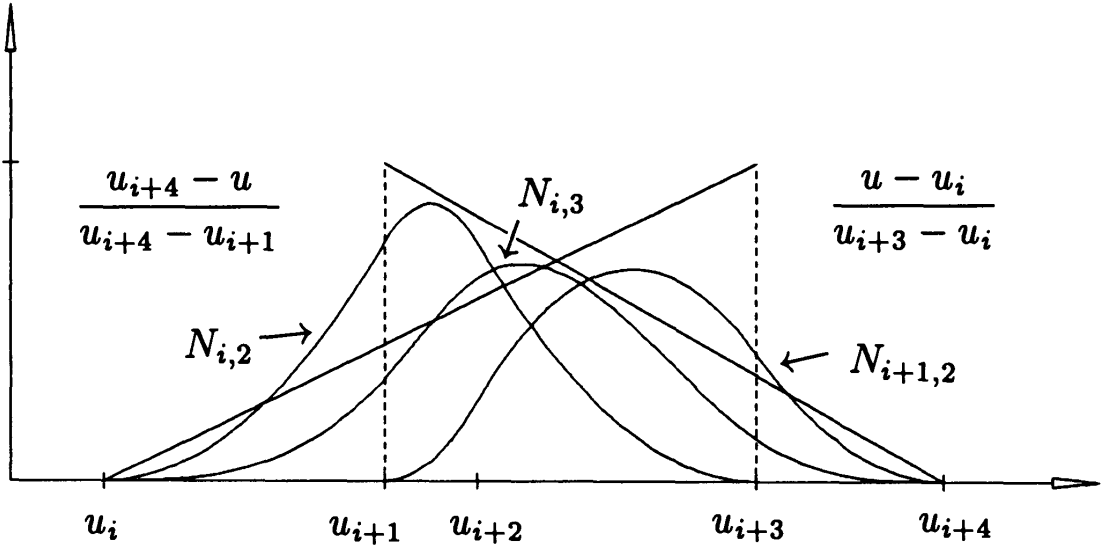
\includegraphics[keepaspectratio, width=10cm]{gambar/Interpolasi/pic3.png}
		\caption{definisi rekursif dari rumus dasar B-spline.}
		\label{gambar:definisirumusdasar}
	\end{figure}
	\item Komputasi dari kumpulan fungsi dasar 
	memerlukan spesifikasi dari sebuah \textit{knot vector}, 
	$U$, dan derajatnya, $p$.
	\item Rumus (\ref{rumusdasarN}) bisa menghasilkan 0/0; 
	nanti hasilnya diubah menjadi nol.
	\item $N_{i,p}(u)$ adalah potongan polinomial, 
	yang didefinisikan pada seluruh garis ril; umumnya 
	hanya pada interval [$u_0$, $u_m$] yang diperhatikan.
	\item interval setengah terbuka, [$u_i, u_{i+1}$), disebut 
	\textit{knot span} ke-$i$; panjangnya bisa nol, 
	karena \textit{knot} tidak perlu dibedakan;
	\item perhitungan fungsi derajat ke-$p$ 
	menghasilkan tabel segitiga terpotong \\
	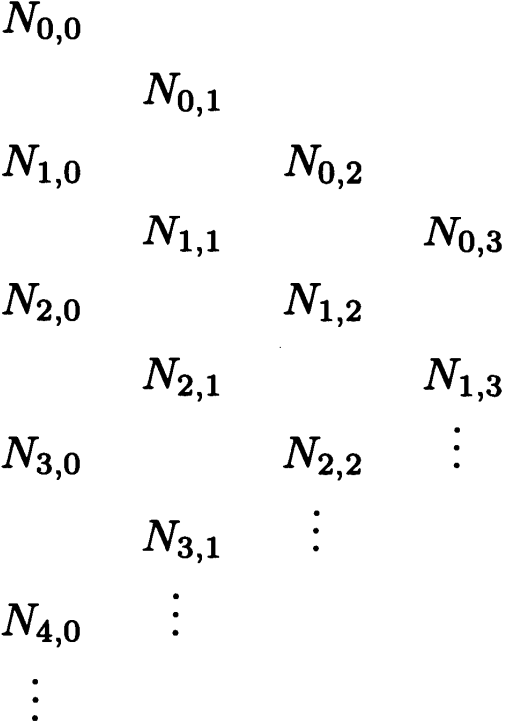
\includegraphics[keepaspectratio, width=4cm]{gambar/Interpolasi/pic4.png}
\end{itemize}

Dengan seluruh hal di atas, penulis mendapatkan 
rumus dasar untuk merubah suatu kurva acak menjadi 
kurva yang memiliki kontinuitas. Bahasan berikut akan 
menyempurnakan rumus dasar untuk memiliki kontinuitas 
yang lebih lanjut.

\subsection{\emph{Global Interpolation}}

Kebanyakan algoritma interpolasi terbagi dalam 
salah satu dari dua kategori: global atau lokal. 
Dengan algoritma global, sistem masalah pada persamaan 
atau optimasi sudah diatur dan diselesaikan. Jika 
data yang diberikan hanya terdiri dari titik dan 
turunan, dan jika yang tidak diketahui hanya 
titik kontrol (derajat, \textit{knot}, dan 
bobot telah dipilih sebelumnya), maka sistem tersebut 
linier dan karenanya akan mudah diselesaikan. Jika data 
yang lebih esoterik, seperti kelengkungan diketahui, 
atau \textit{knot} dan/atau bobot juga tidak diketahui sistemnya, 
maka sistem yang dihasilkan adalah nonlinier. Secara 
teoritis, gangguan pada \textit{input item data} 
siapa pun dapat mengubah bentuk keseluruhan kurva 
atau permukaan; namun, besarnya perubahan menurun 
seiring bertambahnya jarak dari \textit{item data} 
yang terpengaruh. Algoritma lokal lebih bersifat 
geometris, membangun kurva atau segmen permukaan, 
hanya menggunakan data lokal untuk setiap langkah. 
Gangguan pada item data hanya mengubah kurva atau 
permukaan secara lokal. Algoritme ini biasanya lebih 
murah secara komputasi dibandingkan metode global. 
Mereka juga dapat menangani titik puncak, segmen garis 
lurus, dan anomali data lokal lainnya dengan lebih baik. 
Namun, mencapai tingkat kontinuitas yang diinginkan 
pada batas segmen lebih menyusahkan, dan metode lokal 
sering kali menghasilkan banyak \textit{interior knot}.

Berikut merupakan pembentukan rumus interpolasi global.
Misalkan penulis diberikan sekumpulan titik {$\textbf{Q}_k$}, 
$k$ = 0, ..., $n$, dan penulis ingin menginterpolasi 
titik-titik ini dengan kurva \textit{B-spline} 
nonrasional $p$-derajat. Jika ditetapkan nilai 
parameter, $\bar{u}k$, pada masing-masing $\textbf{Q}_k$, 
dan memilih \textit{knot vector} yang sesuai $U = {u_0, ..., u_m}$, 
dapat disiapkan sistem persamaan linier 
(n + 1) variabel dan (n + 1) persamaan:
\begin{equation}
	\textbf{Q}_k = \textbf{C}(u) = \sum_{i = 0}^{n} N_{i,p}(\bar{u}_k) \textbf{P}_i
	\label{rumus:Global}
\end{equation}
Titik kontrol, $\textbf{P}_i$, adalah variabel $n$ + 1 yang 
tidak diketahui. $r$ merupakan jumlah koordinat 
dalam $\textbf{Q}_k$ (biasanya 2, 3, atau 4). 
Perhatikan bahwa metode ini tidak bergantung pada $r$; 
Persamaan (\ref{rumus:Global}) mempunyai satu koefisien 
matriks, dengan $r$ sisi kanan dan, dengan demikian, 
$r$ merupakan himpunan solusi untuk $r$ koordinat dari $\textbf{P}_i$.

Masalah berada dalam pemilihan $\bar{u}_k$ dan $U$, 
dan pilihannya mempengaruhi bentuk dan parameterisasi 
kurva. Sepanjang bagian ini diasumsikan bahwa 
parameternya terletak pada rentang $U \in [0, 1]$. 
Tiga metode umum dalam memilih $\bar{u}_k$ adalah:
\begin{itemize}
	\item \textit{equally spaced}: \\
	\begin{equation}
		\begin{split}
			\bar{u}_0 = 0 \quad & \bar{u}_n = 1 \\
			\bar{u}_k = \frac{k}{n} \quad & k = 1, ..., n-1
		\end{split}
		\label{rumus:equallyspaced}
	\end{equation}
	Metode ini tidak direkomendasikan dikarenakan 
	bisa membuat bentuk yang tak menentu (seperti \textit{loops}) 
	ketika datanya tidak berjarak sama

	\item \textit{chord length}: diumpamakan $d$ 
	merupakan jumlah chord length
	\begin{equation}
		d = \sum_{k=1}^{n}|\textbf{Q}_k - \textbf{Q}_{k-1}|
		\label{chordlength1}
	\end{equation}
	lalu \centerline {\quad $\bar{u}_0 = 0$ \quad $\bar{u}_n = 1$}
	\begin{equation}
		\bar{u}_k = \bar{u}_{k-1} + \frac{|\textbf{Q}_k - \textbf{Q}_{k-1}|}{d} \quad
		k = 1, ..., n-1
		\label{chordlength2}
	\end{equation}
	Ini adalah metode yang paling banyak digunakan, 
	dan secara umum sudah memadai. Hal ini juga 
	memberikan parameterisasi yang "bagus" pada 
	kurva, dalam arti mendekati parameterisasi 
	yang seragam.

	\item metode \textit{centripetal}: umpamakan
	\[d = \sum_{k=1}^{n} \sqrt{|\textbf{Q}_k - \textbf{Q}_{k-1}|} \]
	lalu \centerline {\quad $\bar{u}_0 = 0$ \quad $\bar{u}_n = 1$}
	\begin{equation}
		\bar{u}_k = \bar{u}_{k-1} + \frac{\sqrt{|\textbf{Q}_k - \textbf{Q}_{k-1}|}}{d} \quad
		k = 1, ..., n-1
		\label{centripetal}
	\end{equation}
\end{itemize}

\textit{Knots} bisa berjarak sama, yaitu:
\begin{equation}
	\begin{split}
		u_0 = ... = u_p = 0 \qquad & u_{m-p} = ... = u_m = 1 \\
		u_{j+p} = \frac{j}{n-p+1} \qquad & j = 1, ..., n-p
	\end{split}
	\label{penjarakanknots}
\end{equation}
Namun, cara ini tidak disarankan, jika digunakan 
bersama dengan Persamaan (\ref{chordlength2}) 
atau (\ref{centripetal}) dapat menghasilkan sistem 
persamaan tunggal pada Persamaan \ref{rumus:Global}. 
untuk mengatasinya ada teknik rata-rata sebagai berikut
\begin{equation}
	\begin{split}
		u_0 = ... = u_p = 0 \qquad & u_{m-p} = ... = u_m = 1 \\
		u_{j+p} = \frac{1}{p}\sum_{i=j}^{j+p-1}\bar{u}_i \qquad & j = 1, ..., n-p
	\end{split}
	\label{penjarakanrata_rataknots}
\end{equation}
Dengan metode ini knots mencerminkan distribusi 
$\bar{u}_k$. Selanjutnya menggunakan Persamaan (\ref{penjarakanrata_rataknots}) 
dikombinasikan dengan Persamaan (\ref{chordlength2}) 
atau (\ref{centripetal}) untuk menghitung $\bar{u}_k$ 
mengarah ke sistem (Persamaan \ref{rumus:Global}) 
yang benar-benar positif dan terikat dengan 
\textit{semibandwidth} kurang dari $p$, yaitu, 
$N_{i,p}(\bar{u}_k) = 0$ jika $|i - k| \geq p$. 
Oleh karena itu, penyelesaiannya dapat dilakukan 
dengan eliminasi Gaussian tanpa melakukan \textit{pivoting}.

\begin{figure}[H]
	\centering
	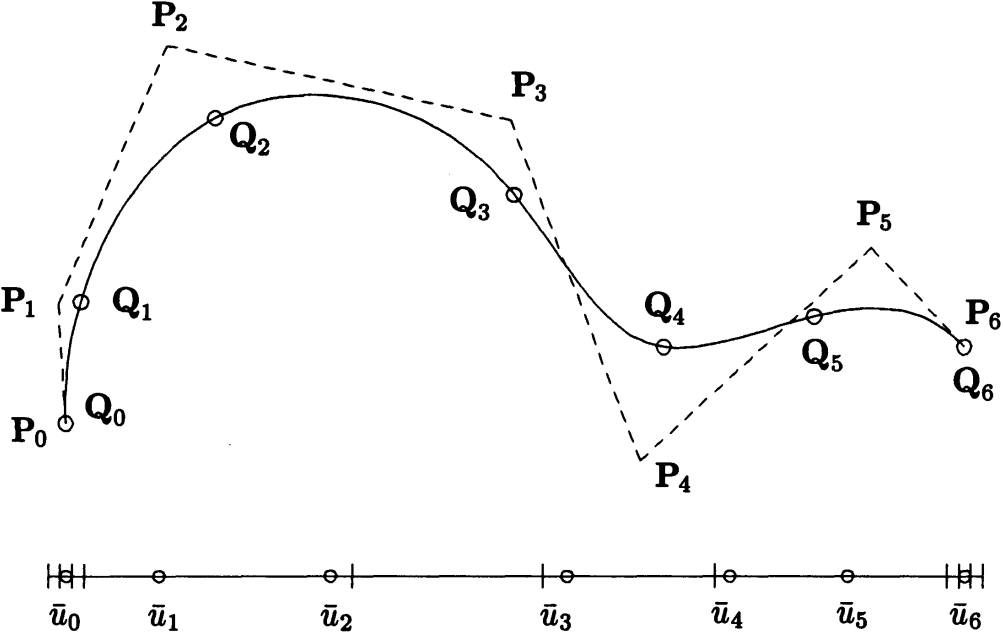
\includegraphics[keepaspectratio, width=10cm]{gambar/Interpolasi/pic5.png}
	\caption{Contoh interpolasi kurva menggunakan 
	parameterisasi \textit{chord length} dan \textit{knot vector}  
	yang diperoleh dengan rata-rata parameter.}
	\label{gambar:contohchordlength}
\end{figure}

Gambar (\ref{gambar:contohchordlength}) menunjukkan titik kontrol, parameter, 
dan \textit{knot vector} dari kurva kubik yang menginterpolasi 
tujuh titik. Parameter ditentukan dengan metode 
\textit{chord length}, dan \textit{knot} diperoleh 
dengan merata-ratakan parameternya (Persamaan \ref{penjarakanrata_rataknots}). 
Pada Gambar (\ref{gambar:interpolasi1}) diilustrasikan perbandingan 
parameterisasi yang berbeda. Gambar 
(\ref{gambar:interpolasi2}) menunjukkan 
perbandingan yang sama dengan menggunakan lebih banyak 
titik data yang tersebar secara "liar". Dalam kedua 
kasus tersebut, kurva kubik dilewatkan melalui tujuh 
titik, menggunakan parameter seragam dan knot seragam 
(kurva padat dan knot vector atas - lihat Persamaan 
[\ref{rumus:equallyspaced}] dan [\ref{penjarakanknots}]); 
parameter \textit{chord length} dan \textit{knot} yang diperoleh 
dengan rata-rata (kurva putus-putus dan \textit{knot vector} 
tengah - lihat Persamaan [\ref{chordlength2}] dan 
[\ref{penjarakanrata_rataknots}]); dan parameter 
sentripetal serta knot yang diperoleh dengan 
rata-rata (kurva titik-titik dan knot vector 
bawah - lihat Persamaan [\ref{centripetal}] dan 
[\ref{penjarakanrata_rataknots}]). Perhatikan akan 
Gambar (\ref{gambar:interpolasi2}) bagaimana 
\textit{chord length} dan kurva 
parameter sentripetal beradaptasi dengan perubahan 
jarak titik.

\begin{figure}[H]
	\centering
	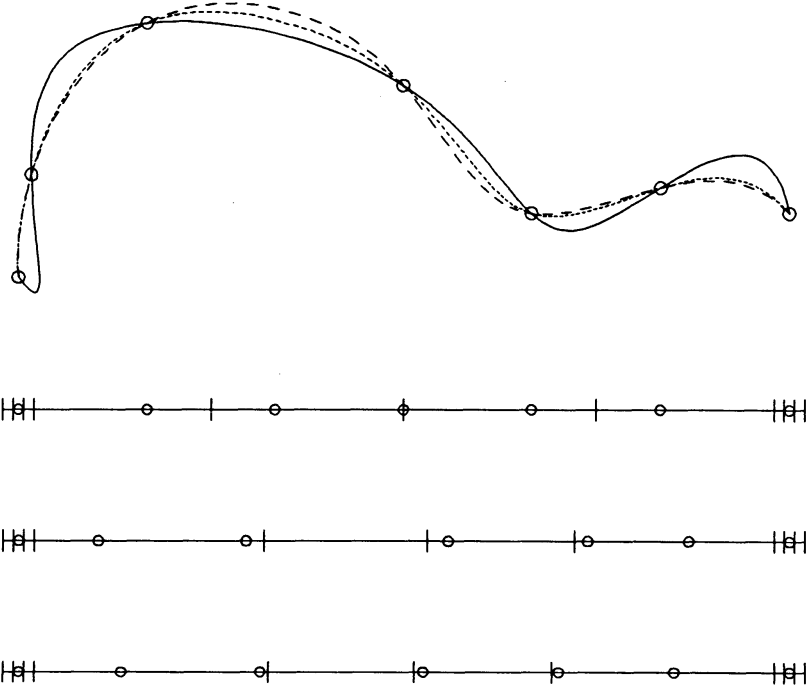
\includegraphics[keepaspectratio, width=10cm]{gambar/Interpolasi/pic6.png}
	\caption{Contoh interpolasi kurva dengan 
	parameterisasi dan \textit{knot vector}  berbeda.}
	\label{gambar:interpolasi1}
\end{figure}

\begin{figure}[H]
	\centering
	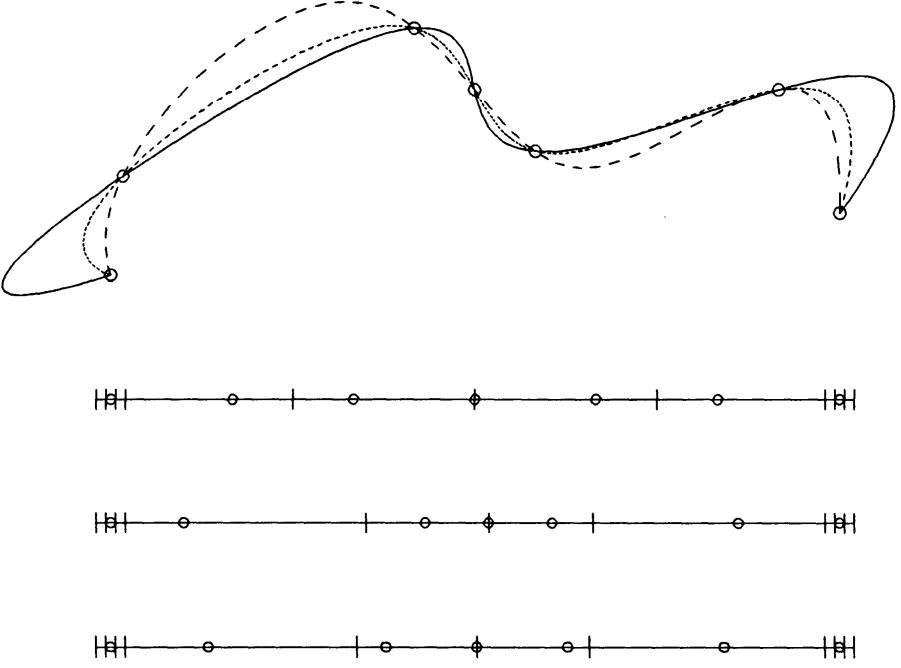
\includegraphics[keepaspectratio, width=10cm]{gambar/Interpolasi/pic7.png}
	\caption{Contoh interpolasi kurva dengan 
	parameterisasi dan \textit{knot vector}  berbeda.}
	\label{gambar:interpolasi2}
\end{figure}

Gambar (\ref{gambar:interpolasi3}) mengilustrasikan 
interpolasi dengan derajat yang berbeda-beda; 
kurva padat, putus-putus, dan putus-putus 
masing-masing memiliki derajat 2, 3, dan 4. 
Gambar (\ref{gambar:interpolasi4}) menunjukkan 
ketidakmampuan interpolasi global untuk menangani 
kumpulan titik kolinear.

\begin{figure}[H]
	\centering
	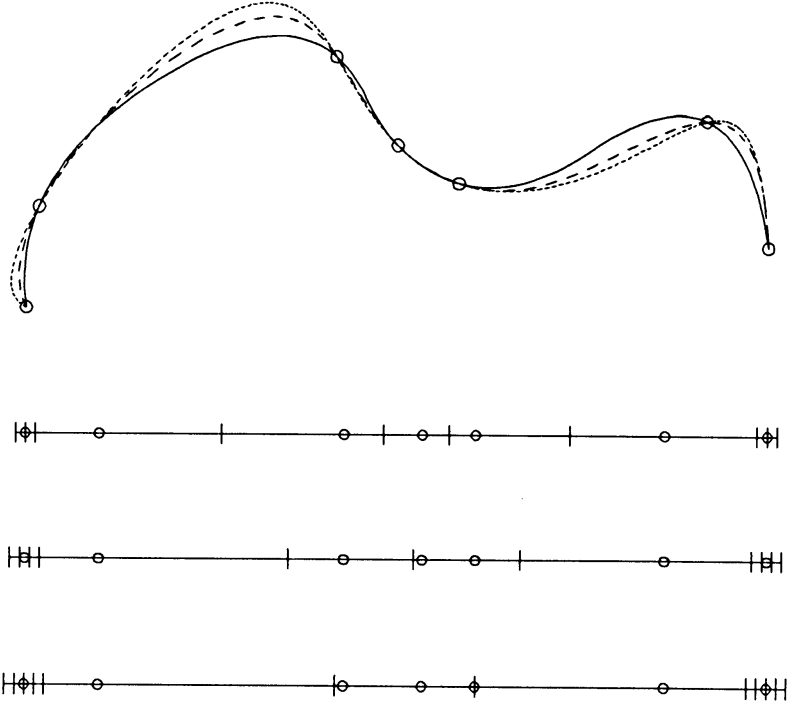
\includegraphics[keepaspectratio, width=10cm]{gambar/Interpolasi/pic8.png}
	\caption{Interpolasi kurva dengan derajat 
	berbeda menggunakan parameterisasi chord 
	length dan knot yang diperoleh dengan rata-rata.}
	\label{gambar:interpolasi3}
\end{figure}

\begin{figure}[H]
	\centering
	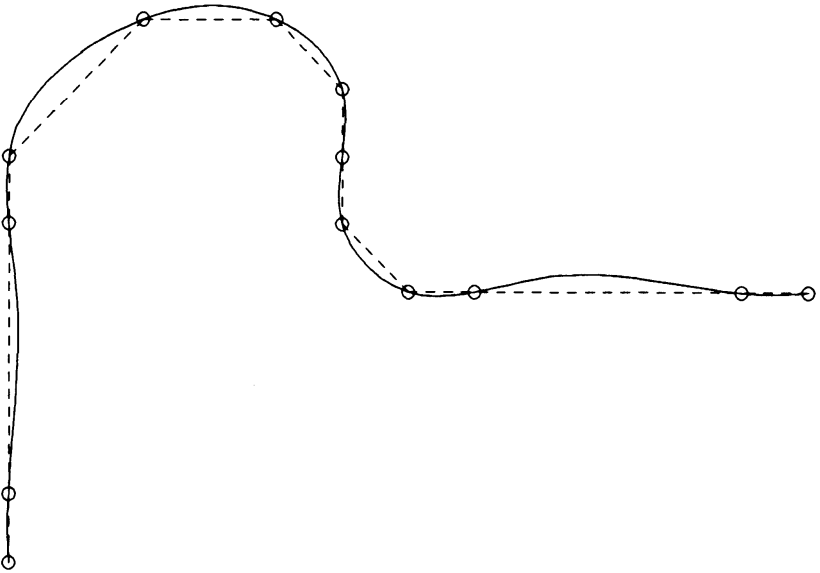
\includegraphics[keepaspectratio, width=10cm]{gambar/Interpolasi/pic9.png}
	\caption{Interpolasi kurva kubik global 
	ke data yang berisi titik-titik kolinear 
	(lihat garis putus-putus).}
	\label{gambar:interpolasi4}
\end{figure}
Setelah $\bar{u}_k$ dan \textit{knot} dihitung, matriks koefisien 
$(n+1)$ x $(n+1)$ dari sistem (Persamaan \ref{rumus:Global}) 
dibuat dengan mengevaluasi fungsi basis bukan nol pada 
setiap $\bar{u}_k, k = 0, . ..., n$.

\textbf{Contoh:}

Misalkan {$\textbf{Q}_k$} = {(0, 0), (3, 4), (-1, 4), 
(-4, 0), (-4, -3)}, dan asumsikan penulis ingin 
menginterpolasi $\textbf{Q}_k$ dengan kurva kubik. 
Digunakan persamaan (\ref{chordlength2}) dan 
(\ref{penjarakanrata_rataknots}) untuk menghitung 
$\bar{u}_k$ dan $u_j$, dan kemudian membuat sistem persamaan 
linier, Persamaan (\ref{rumus:Global}). \textit{chord lengths} 
yang terpisah adalah

\centerline{$|\textbf{Q}_1 - \textbf{Q}_0| = 5$ \quad
$|\textbf{Q}_2 - \textbf{Q}_1| = 4$ \quad
$|\textbf{Q}_3 - \textbf{Q}_2| = 5$ \quad
$|\textbf{Q}_4 - \textbf{Q}_3| = 3$}

Dan jumlah \textit{chord length} menjadi $d = 17$, maka

\centerline{$\bar{u}_0 = 0$ \quad
$\bar{u}_1 = \frac{5}{17}$ \quad
$\bar{u}_2 = \frac{9}{17}$ \quad
$\bar{u}_3 = \frac{14}{17}$ \quad
$\bar{u}_4 = 1$}
Gunakan rumus (\ref{penjarakanrata_rataknots})
\[u_4 = \frac{1}{3}(\frac{5}{17}+\frac{9}{17}+\frac{14}{17})=\frac{28}{51} \]
maka \[U = \{0,0,0,0,\frac{28}{51},1,1,1,1\}\]
Sistem persamaan linearnya adalah
\[ \begin{split}
	\begin{bmatrix}
	1 & 0 & 0 & 0 & 0\\ 
	N_{0,3}(\frac{5}{17}) & N_{1,3}(\frac{5}{17}) & N_{2,3}(\frac{5}{17}) & N_{3,3}(\frac{5}{17}) & 0\\ 
	N_{0,3}(\frac{9}{17}) & N_{1,3}(\frac{9}{17}) & N_{2,3}(\frac{9}{17}) & N_{3,3}(\frac{9}{17}) & 0\\ 
	0 & N_{1,3}(\frac{14}{17}) & N_{2,3}(\frac{14}{17}) & N_{3,3}(\frac{14}{17}) & N_{4,3}(\frac{14}{17})\\ 
	0 & 0 & 0 & 0 & 1
	\end{bmatrix} &
	\begin{bmatrix}
		\textbf{P}_0 \\
		\textbf{P}_1 \\
		\textbf{P}_2 \\
		\textbf{P}_3 \\
		\textbf{P}_4 
	\end{bmatrix}
	\\
	= & \begin{bmatrix}
		\textbf{Q}_0 \\
		\textbf{Q}_1 \\
		\textbf{Q}_2 \\
		\textbf{Q}_3 \\
		\textbf{Q}_4
	\end{bmatrix}
	\end{split}
\]

\subsection{\emph{Local Interpolation}}

Seperti yang dikatakan sebelumnya, interpolasi global 
tidak memberikan hasil yang sempurna, karena rumus nya terlalu 
mengeneralisir pemindahan \textit{knot vector}. 
Untuk mengatasi hal itu, 
digunakan interpolasi lokal. Misalkan {$Q_k$} , $k = 0, ..., n$, 
diberikan. Yang dimaksud dengan interpolasi kurva lokal adalah 
metode yang membentuk $n$ segmen kurva polinomial atau rasional, 
$C_{i}(u), i = 0, ..., n - 1$, sehingga $Q_i$ dan $Q_{i+1}$ 
adalah titik akhir dari $C_{i}(u)$. Segmen-segmen yang 
berdekatan digabungkan dengan tingkat kontinuitas 
tertentu, dan konstruksi berlangsung berdasarkan segmen, 
umumnya dari kiri ke kanan. Persamaan apa pun yang muncul 
bersifat lokal hanya pada beberapa segmen yang berdekatan. 
Dalam \textit{framework} NURBS, mereka membuat segmen menggunakan 
kurva Bézier polinomial atau rasional, kemudian memperoleh 
kurva NURBS dengan memilih \textit{knot vector} yang sesuai.

\begin{figure}[H]
	\centering
	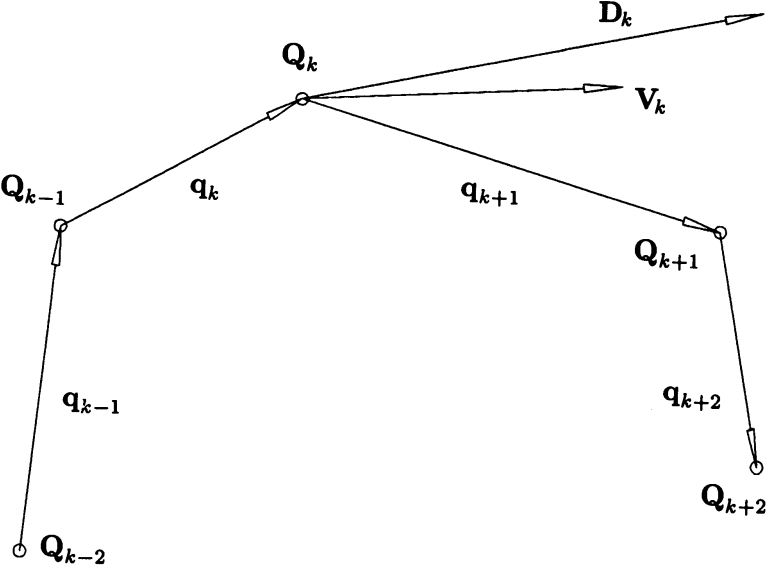
\includegraphics[keepaspectratio, width=10cm]{gambar/Interpolasi/pic10.png}
	\caption{Perhitungan vektor tangen ($\textbf{V}_k$) dan 
	turunan ($\textbf{D}_k$) untuk interpolasi kurva lokal.}
	\label{gambar:arahtangendanturunan}
\end{figure}

Sekarang misalkan $\bar{u}_i$ menyatakan parameter awal 
$\textbf{C}_{i}(u)$ dan parameter akhir $\textbf{C}_{i-1}(u)$. 
$\textbf{C}_{i}(u)$ dan $\textbf{C}_{i-1}(u)$. bertemu di 
$\bar{u}_i$ dengan kontinuitas $G^1$ (G untuk geometri) 
jika arah singgungnya berimpit di sana, yaitu jika 
$\textbf{C}'_{i}(\bar{u}_i)$ dan $\textbf{C}'_{i-1}(\bar{u}_i)$ 
menunjuk ke arah yang sama. Namun, besarnya mungkin berbeda. 
Kontinuitas $G^1$ menyiratkan bahwa kurva tersebut 
secara visual kontinu (halus) tetapi mungkin memiliki 
diskontinuitas dalam parameterisasinya. Algoritma 
interpolasi lokal dirancang untuk memberikan tingkat 
kontinuitas $G$ atau $C$ tertentu; dalam sub bab ini 
hanya menyajikan algoritma yang menyediakan 
kontinuitas $G^1$ atau $C^1$. Metode lokal yang 
menghasilkan kontinuitas lebih tinggi tidak 
banyak digunakan. Meskipun $G^2$ dan $C^2$ dimungkinkan 
dengan kubik, derajat yang lebih tinggi harus 
digunakan jika fleksibilitas yang wajar ingin dipertahankan.

Untuk mendapatkan segmen Bézier, $\textbf{C}_{i}(u)$, 
memerlukan komputasi titik kontrol Bézier bagian dalam, 
satu titik untuk kuadrat, dua untuk kubik. Titik kendali 
ini terletak pada garis singgung(\textit{tangent}) kurva di 
$\textbf{Q}_k$; oleh karena itu, diperlukan vektor 
singgung(\textit{tangent vector}) $\textbf{T}_k$ pada 
setiap $\textbf{Q}_k$. Dalam beberapa kasus, vektor 
tersebut dapat dimasukkan bersama dengan $\textbf{Q}_k$; 
misalnya, persamaan tersebut mudah diperoleh saat 
menghitung titik potong antara dua permukaan. Namun, 
jika tidak dimasukkan maka harus dihitung sebagai bagian 
dari algoritma interpolasi. Ada sejumlah metode; Boehm 
[\cite{BOHM19841}] memberikan survei tentang berbagai 
metode. Misalkan
\[\Delta\bar{u}_k = \bar{u}_k - \bar{u}_{k-1} \quad
\textbf{q}_k = \textbf{Q}_k - \textbf{Q}_{k-1} \quad
\textbf{d}_k = \frac{\textbf{q}_k}{\Delta\bar{u}_k}
\]
Semua metode memiliki satu dari dua bentuk
\begin{equation}
	\textbf{D}_k = (1 - \alpha_k)\textbf{d}_k = \alpha_{k}\textbf{d}_{k+1}
	\label{rumus:turunanlokal} 
\end{equation}
atau
\begin{equation}
	\textbf{T}_k = \frac{\textbf{V}_k}{|\textbf{V}_k|} \quad
	\textbf{V}_k = (1 - \alpha_k)\textbf{q}_k + \alpha_{k}\textbf{q}_{k+1}
	\label{rumus:tangenlokal} 
\end{equation}
(lihat Gambar \ref{gambar:arahtangendanturunan}). 
Perhatikan bahwa Persamaan (\ref{rumus:turunanlokal}) 
mengasumsikan bahwa nilai $\bar{u}_k$ telah ditetapkan. 
Vektor $\textbf{D}_k$ dapat dipandang sebagai perkiraan 
turunannya. Persamaan (\ref{rumus:tangenlokal}) tidak 
menggunakan parameter $\bar{u}_k$ dan vektor yang 
dihasilkan harus dipandang sebagai arah singgung saja. 
Penetapan besaran dan parameter harus dilakukan bersamaan 
satu sama lain karena tidak independen. Perhatikan 
juga bahwa ini menggunakan notasi $\textbf{T}$ hanya 
untuk vektor singgung satuan panjang. Persamaan 
(\ref{rumus:turunanlokal}) dan (\ref{rumus:tangenlokal}) 
merupakan interpolasi linier. Berbagai skema berbeda 
dalam cara mereka mengkomputasi parameter interpolasi 
$\alpha_k$ yang biasanya bergantung pada tiga atau 
lima titik tetangga. Misalnya, metode Bessel [\cite{DeBoor}] 
adalah metode tiga titik menggunakan
\begin{equation}
	\alpha_k = \frac{\Delta\bar{u}_k}
	{\Delta\bar{u}_k + \Delta\bar{u}_{k+1}} \quad
	k = 1,...,n-1
	\label{rumus:alfalokal} 
\end{equation}
Bersama dengan persamaan (\ref{rumus:turunanlokal}) digabungkan menjadi
\begin{equation}
	\alpha_k = \frac{\left | \textbf{q}_{k-1} * \textbf{q}_k \right |}
	{\left | \textbf{q}_{k-1}*\textbf{q}_k \right | + 
	\left | \textbf{q}_{k+1}*\textbf{q}_{k+2} \right |} \quad
	k = 2,...,n-2
	\label{rumus:alfalokal2} 
\end{equation}
bersama dengan Persamaan (\ref{rumus:tangenlokal}) 
menghasilkan metode lima poin untuk memperoleh $\textbf{T}_k$. 
Keuntungannya adalah tiga titik yang segaris, $\textbf{Q}_{k-1}, 
\textbf{Q}_k, \textbf{Q}_{k+1}$, menghasilkan $\textbf{T}_k$ yang 
sejajar dengan ruas garis. Penyebut Persamaan 
(\ref{rumus:alfalokal2}) hilang jika $\textbf{Q}_{k-2}, 
\textbf{Q}_{k-1}, \textbf{Q}_k$ segaris dan $\textbf{Q}_k, 
\textbf{Q}_{k+1}, \textbf{Q}_{k+2}$ segaris. Ini 
menyiratkan antara adanya sudut di $\textbf{Q}_k$ atau 
ada segmen garis lurus dari $\textbf{Q}_{k-2}$ sampai 
$\textbf{Q}_{k+2}$. Dalam kasus ini $\alpha_k$ dapat 
didefinisikan dalam beberapa cara; yaitu
\begin{itemize}
	\item $\alpha_k$ = 1, yang berarti $\textbf{V}_k$ = 
	$\textbf{q}_{k+1}$, ini menghasilkan sudut di 
	$\textbf{Q}_k$ jika tersirat dalam data
	\item $\alpha_k$ = 1/2, yang berarti $\textbf{V}_k$ = 
	$\frac{1}{2}(\textbf{q}_k+\textbf{q}_{k+1})$; 
	pilihan ini menghaluskan suatu sudut jika tersirat.
\end{itemize}
Berdasarkan cara di atas, rutinitas interpolasi 
kurva lokal dapat diterima dengan tanda masukan(\textit{flag}), 
yang menunjukkan apakah akan dipertahankan sudutnya 
atau tidak. Semua metode memerlukan perlakuan khusus 
pada ujungnya. Untuk skema tiga titik bisa dibuat
\begin{equation}
	\textbf{D}_0 = 2\textbf{d}_1 - \textbf{D}_1 \quad
	\textbf{D}_n = 2\textbf{d}_n - \textbf{D}_{n-1}
	\label{rumus:turunantigatitik} 
\end{equation}
Dan untuk skema lima titik bisa dipakai
\begin{equation}
	\begin{split}
		\textbf{q}_0 = 2\textbf{q}_1 - \textbf{q}_2 \quad & 
		\textbf{q}_{-1} = 2\textbf{q}_0 - \textbf{q}_1 \\
		\textbf{q}_{n+1} = 2\textbf{q}_n - \textbf{q}_{n-1} \quad & 
		\textbf{q}_{n+2} = 2\textbf{q}_{n+1} - \textbf{q}_n
	\end{split}
	\label{rumus:turunanlimatitik}
\end{equation}
untuk dimasukkan ke dalam Persamaan (\ref{rumus:alfalokal2}) 
dan (\ref{rumus:tangenlokal}) sehingga diperoleh 
$\textbf{T}_0, \textbf{T}_1$ dan 
$\textbf{T}_{n-1}, \textbf{T}_n$. 
selanjutnya akan menjelaskan interpolasi 
permukaan lokal bikubik

Misalkan {$\textbf{Q}_{k,l}$}, $k = 0, ..., n$ 
dan $l = 0, ..., m$, adalah himpunan titik data, 
dan misalkan {($\bar{u}_k, \bar{v}_k$)} adalah 
pasangan parameter yang bersesuaian, dihitung dengan 
rata-rata chord length (seperti pada Algoritma 
(\ref{chordlength2})). Metode berikut menghasilkan 
permukaan bikubik, $\textbf{S}(u, v)$, yaitu

\begin{equation}
	\textbf{S}(\bar{u}_k, \bar{v}_l) = 
	\sum_{i=0}^{2n+1}\sum_{j=0}^{2m+1}
	N_{i,3}(\bar{u}_k)N_{j,3}(\bar{v}_k)\textbf{P}_{i,j}
	\label{rumus:localbicubic} 
\end{equation}
diperoleh permukaan dengan membuat tambalan Bézier bikubik $nm$, 
$\{\textbf{B}_{k,l}(u, v)\}, k = 0, ..., n-1, l = 0, ... , m-1$, 
di mana $\textbf{Q}_{k,l}, \textbf{Q}_{k+1,l}, 
\textbf{Q}_{k,l+1}, \textbf{Q}_{k+1,l+1}$ adalah 
titik sudut tambalan, dan tambalan bergabung dengan 
kontinuitas $C^{1,1}$ melintasi batasnya. Kecuali batas 
permukaan, semua baris dan kolom titik kontrol yang 
berisi {$\textbf{Q}_{k,l}$} asli dihilangkan 
(lihat Gambar (\ref{gambar:beziernet}) 
dan (\ref{gambar:beziernetdetail})), menyisakan $(2n + 2)(2m + 2)$ 
titik kontrol di \textit{B-spline} permukaan \textit{spline}. 
\textit{Knot vector}-nya adalah
\begin{equation}
	\begin{split}
		U = \{0,0,0,0,\bar{u}_1,\bar{u}_1,\bar{u}_2,\bar{u}_2,...,
		\bar{u}_{n-1},\bar{u}_{n-1},1,1,1,1\} \\
		V = \{0,0,0,0,\bar{v}_1,\bar{v}_1,\bar{v}_2,\bar{v}_2,...,
		\bar{v}_{m-1},\bar{v}_{m-1},1,1,1,1\}
	\end{split}
	\label{rumus:knotvectorbicubic} 
\end{equation}

\begin{figure}[H]
	\centering
	\begin{subfigure}{.5\textwidth}
		\centering
		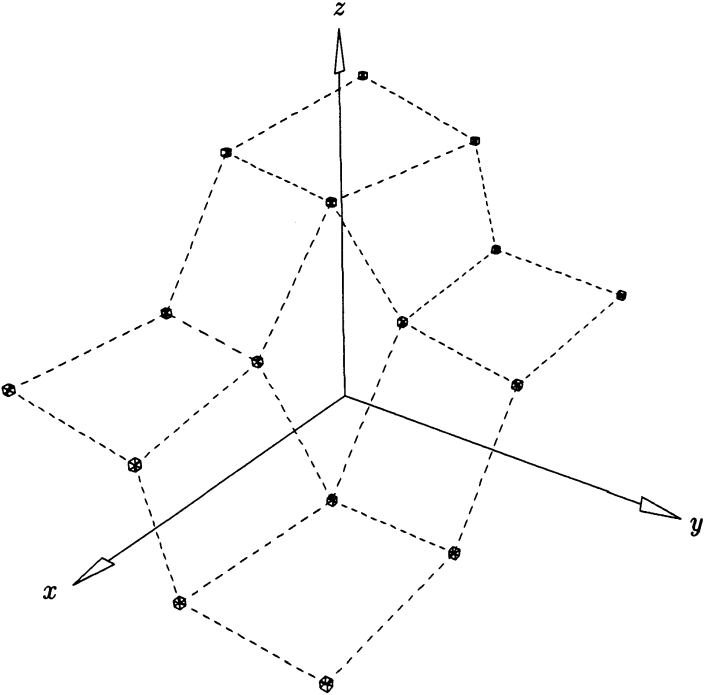
\includegraphics[keepaspectratio, width=5cm]{gambar/Interpolasi/pic11.png}
		\caption{\textit{Data set}}
		\label{gambar:datasetlocal}
	\end{subfigure}%
	\begin{subfigure}{.5\textwidth}
		\centering
		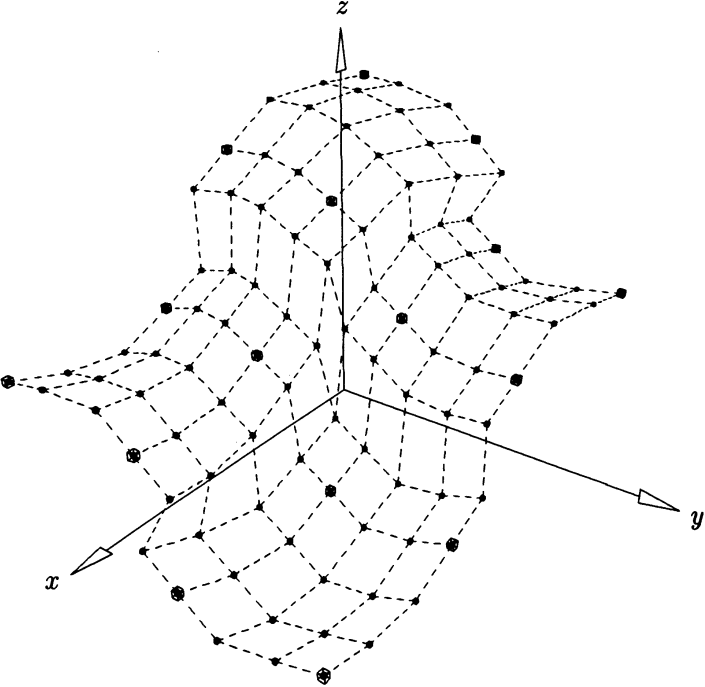
\includegraphics[keepaspectratio, width=5cm]{gambar/Interpolasi/pic12.png}
		\caption{jaring Bézier dari interpolant}
		\label{gambar:beziernet}
	\end{subfigure} \\
	\begin{subfigure}{.5\textwidth}
		\centering
		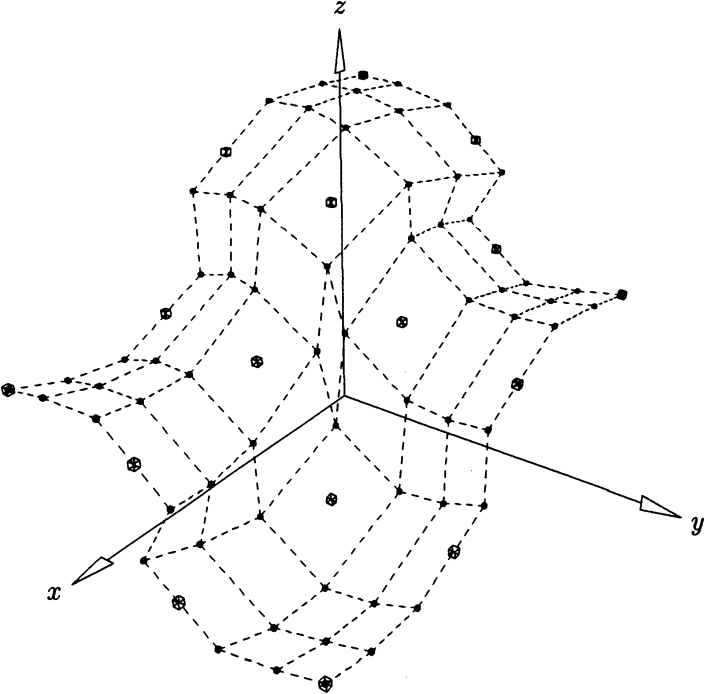
\includegraphics[keepaspectratio, width=5cm]{gambar/Interpolasi/pic13.png}
		\caption{jaring \textit{B-spline} (lingkaran besar menandai 
		titik data, dan lingkaran kecil menandai titik 
		kontrol \textit{B-spline})}
		\label{gambar:beziernetdetail}
	\end{subfigure}%
	\begin{subfigure}{.5\textwidth}
		\centering
		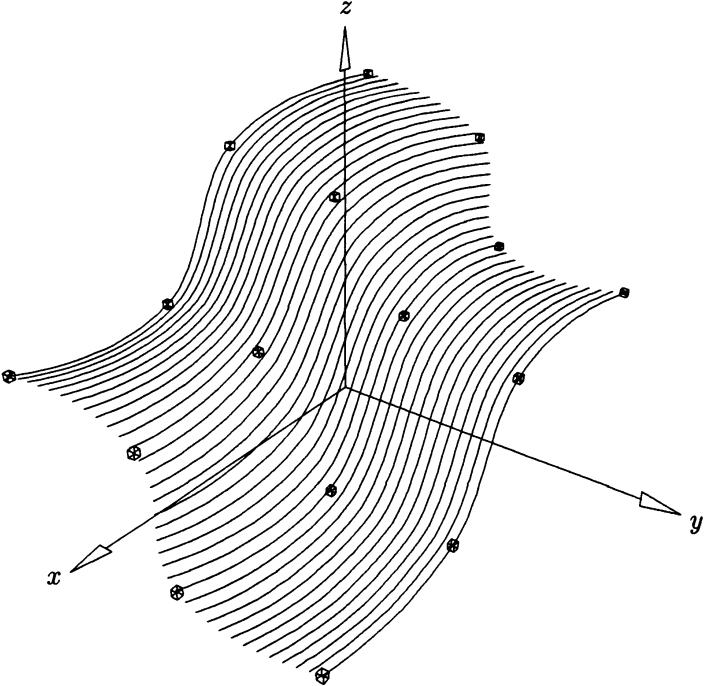
\includegraphics[keepaspectratio, width=5cm]{gambar/Interpolasi/pic14.png}
		\caption{interpolsi permukaan.}
		\label{gambar:surfaceinterpolant}
	\end{subfigure}
	\caption{$C^{(1,1)}$ Interpolasi permukaan bikubik lokal}
\end{figure}

Tambalan bikubik Bézier memiliki 16 titik kontrol. 
12 titik kontrol perbatasan diperoleh dengan awalnya 
melakukan looping melalui $m + 1$ baris dan $n + 1$ 
kolom data dan menggunakan skema interpolasi kurva 
kubik. Skemanya sedikit berbeda dengan detail 
sebelumnya, karena sudah mempunyai parameternya 
{$(\bar{u}_k, \bar{v}_k)$}. Perhatikan bahwa ini harus 
dikomputasi terlebih dahulu, karena semua baris (kolom) 
harus memiliki parameterisasi yang sama pada permukaan 
produk tensor. Dengan demikian, masih dapat 
memaksakan kontinuitas $C^1$ pada titik akhir segmen, 
namun tidak dapat dipaksakan kecepatan yang 
sama pada titik tengah segmen kurva Bézier. Lebih 
spesifik lagi, misalkan $l = l_0$ tetap, dan perhatikan 
kurva kubik yang menginterpolasi titik-titik $\textbf{Q}_{0,l_0} 
, ..., \textbf{Q}_{n,l_0}$. Misalkan $r_{l_0}$ menyatakan 
jumlah chord length pada baris ke-$l_0$. Pada setiap titik, 
$\textbf{Q}_{k,l_0}$, hitung $\textbf{T}_{k,l_0}^u$, 
(satuan tangen pada arah $u$) seperti sebelumnya 
(Persamaan (\ref{rumus:tangenlokal}), (\ref{rumus:alfalokal2}), 
dan (\ref{rumus:turunanlimatitik})). Kemudian titik-titik 
\textit{interior} Bézier pada baris ini dikomputasi dengan
\begin{equation}
	\textbf{P}_{1,0}^{k,l_0}=\textbf{Q}_{k,l_0}+a\textbf{T}_{k,l_0}^u \quad
	\textbf{P}_{2,0}^{k,l_0}=\textbf{Q}_{k+1,l_0}+a\textbf{T}_{k+1,l_0}^u 	
\end{equation}
dimana \[a=\frac{r_{l_0}(\bar{u}_{k+1}-\bar{u}_k)}{3}=
\frac{r_{l_0}\Delta\bar{u}_{k+1}}{3}\]
Kurva yang dihasilkan adalah kontinu $C^1$, dengan 
besaran turunan sama dengan $r_{l_0}$ pada semua 
$\textbf{Q}_{k,l_0}$. Teknik yang sama diterapkan 
pada $n + 1$ kolom data.

ini kembali pada menghitung \textit{interior} empat 
titik kontrol dari setiap patch Bézier. Hal ini memerlukan 
estimasi untuk turunan parsial campuran, $\textbf{D}_{k,l}^{uv}$, 
pada setiap $\textbf{Q}_{k,l}$. diperoleh 
rumus untuk $\textbf{Q}_{k,l}$ berdasarkan metode 
tiga titik Bessel (Persamaan (\ref{rumus:turunanlokal}), 
(\ref{rumus:alfalokal}), dan (\ref{rumus:turunantigatitik})). 
Misalkan $r_l$ dan $s_k$ menyatakan jumlah \textit{chord length} 
pada baris ke-$l$ (kolom ke-$k$). Kemudian
\begin{equation}
	\textbf{D}_{k,l}^u = r_l \textbf{T}_{k,l}^u \quad
	\textbf{D}_{k,l}^v = s_k \textbf{T}_{k,l}^v 
\end{equation}
lalu bentuk \[\textbf{d}_{k,l}^{vu} = 
(1-\alpha_k)\frac{\textbf{D}_{k,l}^v - \textbf{D}_{k-1,l}^v}
{\Delta\bar{u}_k} + \alpha_k \frac{\textbf{D}_{k+1,l}^v - 
\textbf{D}_{k,l}^v}{\Delta\bar{u}_{k+1}} \]
dan \[\textbf{d}_{k,l}^{uv} = 
(1-\beta_l)\frac{\textbf{D}_{k,l}^u - \textbf{D}_{k,l-1}^u}
{\Delta\bar{v}_l} + \beta_l \frac{\textbf{D}_{k,l+1}^u - 
\textbf{D}_{k,l}^u}{\Delta\bar{v}_{l+1}} \]
dengan \[\alpha_k = \frac{\Delta\bar{u}_k}
{\Delta\bar{u}_k + \Delta\bar{u}_{k+1}} \quad
\beta_l = \frac{\Delta\bar{v}_l}
{\Delta\bar{v}_l + \Delta\bar{v}_{l+1}}\]
menjadi
\begin{equation}
	\textbf{D}_{k,l}^{uv} = \frac{\alpha_k \textbf{d}_{k,l}^{uv} +
	\beta_l \textbf{d}_{k,l}^{vu}}{\alpha_k + \beta_l}
	\label{rumus:turunanterakhir}
\end{equation}

Rumus akhir yang sesuai (Persamaan (\ref{rumus:turunantigatitik})) 
harus digunakan pada pembatasnya. Empat \textit{interior} 
titik kontrol pada tambalan ke-($k, l$) sekarang 
dihitung menggunakan Persamaan. (\ref{rumus:turunanterakhir})
\begin{equation}
	\begin{split}
		\textbf{P}_{1,1}^{k,l} &= \gamma\textbf{D}_{k,l}^{uv} + 
		\textbf{P}_{0,1}^{k,l} + \textbf{P}_{1,0}^{k,l} -
		\textbf{P}_{0,0}^{k,l} \\%1
		\textbf{P}_{2,1}^{k,l} &= -\gamma\textbf{D}_{k+1,l}^{uv} + 
		\textbf{P}_{3,1}^{k,l} - \textbf{P}_{3,0}^{k,l} + 
		\textbf{P}_{2,0}^{k,l} \\%2
		\textbf{P}_{1,2}^{k,l} &= -\gamma\textbf{D}_{k,l+1}^{uv} + 
		\textbf{P}_{1,3}^{k,l} - \textbf{P}_{0,3}^{k,l} + 
		\textbf{P}_{0,2}^{k,l} \\%3
		\textbf{P}_{2,2}^{k,l} &= \gamma\textbf{D}_{k+1,l+1}^{uv} + 
		\textbf{P}_{2,3}^{k,l} + \textbf{P}_{3,2}^{k,l} -
		\textbf{P}_{3,3}^{k,l} %4
	\end{split}
\end{equation}
dimana \[\gamma = \frac{\Delta\bar{u}_k+1
\Delta\bar{v}_l+1}{9}\]

% Baris ini digunakan untuk membantu dalam melakukan sitasi
% Karena diapit dengan comment, maka baris ini akan diabaikan
% oleh compiler LaTeX.
\begin{comment}
\bibliography{daftar-pustaka}
\end{comment}
%!TEX root = ./template-skripsi.tex
%-------------------------------------------------------------------------------
%                     BAB III
%               			PEMBAHASAN
%-------------------------------------------------------------------------------
% \SetKwComment{Comment}{/* }{ */}
\chapter{METODOLOGI PENELITIAN}

\section{Perancangan Sistem}

Penulis merancang sistem ini berdasarkan dari 
penelitian Rizki, yaitu untuk pendeteksian luka. 
Yang membuat penelitian ini berbeda dengan penelitian 
Rizki adalah interpolasi yang dipakai adalah buatan 
penulis dengan referensi NURBS, lalu menggantikan 
\textit{active contour} dengan \textit{border following} 
yang ditulis oleh Hafizhun Alim(\cite{Hafizhun}). berikut merupakan diagram 
alir penelitian yang akan dilakukan.

\begin{figure}[H]
	\centering
	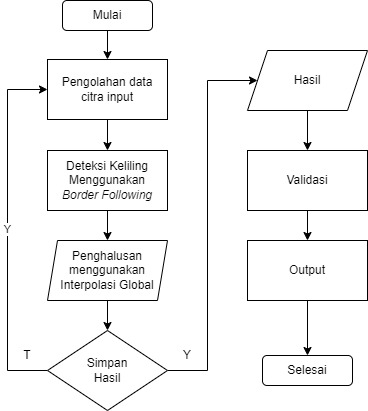
\includegraphics[keepaspectratio,width = 7cm]{gambar/Bab3Extra/Diagram_alur.jpg}
	\caption{Diagram alir penelitian}
	\label{diagramalur}
\end{figure}

\begin{algorithm}[H]
  \caption{\textit{Main}}
  \begin{algorithmic}[1]
  \Require{Image, $p$}
  \Ensure{Curve Points}
  \Function{Main}{Image, $p$}
    \State image $\gets$ imread(Image) \Comment read image as value
    \State points $\gets$ BorderFollowing(image) \Comment algorithm(\ref{algoritma:BorderFollowing})
    \State curve $\gets$ GlobalInterpolation(points, $p$) \Comment algorithm(\ref{algoritma:globalinterpolation})
    \State Results $\gets$ Image + curve \Comment put curve to image
    \State \Return Results
  \EndFunction
  \end{algorithmic}
  \label{algoritma:main}
\end{algorithm}

\section{\textit{Border Following}}

Setelah citra diolah 

Setelah merubah gambarnya dengan Interpolasi, penulis 
akan menggunakan teknik \textit{border following} untuk membuat garis 
pada gambar. \textit{Border following} merupakan teknik yang diusulkan 
oleh Satoshi Suzuki dan Keichi Abe di mana teknik ini menelusuri 
batas suatu objek dengan mengikuti transisi antara piksel latar 
depan (objek) dan latar belakang pada gambar lalu memberikan 
definisi derajat pada piksel. Algoritma \textit{border following} bekerja 
dengan memulai pada titik tertentu pada batas suatu objek dan 
kemudian mengikuti batas tersebut searah atau berlawanan 
arah jarum jam dengan mengidentifikasi titik berikutnya di 
sepanjang batas tersebut.

Algoritma ini dimulai dengan mengasumsikan citra yang 
dimasukkan merupakan citra biner dengan latar belakang 
merupakan piksel bernilai 0 dan latar depan (objek) 
sebagai piksel bernilai 1. Lalu dilanjutkan dengan 
memberi masukan berupa citra biner dari proses operasi 
morfologi yang dilanjutkan denang proses memindai(scan) 
dimulai dari piksel paling kiri atas. Apabila sudah memindai
sampai piksel ($i, j$) bernilai $f_{i,j} \neq 0$ (bukan latar
belakang), ditentukan piksel tersebut apakah merupakan 
\textit{starting point}  dari operasi \textit{border following}
untuk tepi luar atau tepi dalam (gambar \ref{gambar:kondisi_batas}).
Lalu menentukan \textit{parent border} untuk piksel 
(i,j) berdasarkan gambar (\ref{gambar:hasil_penciutan_blob}).
Dilanjutkan dengan melakukan \textit{border following} dimulai 
dari \textit{starting point} piksel (i, j) sampai 
\textit{pointer} kembali ke posisi \textit{starting point}.
Algoritma yang dipakai adalah algoritma kedua Suzuki(\cite{Suzuki})
maka nilai $N B D$ dan $- N B D$ akan di-set 
masing-masing 2 dan -2. lalu pemindai akan melanjutkan pemindaian
untuk mencari objek ($f_{i,j} \neq 0$). Algoritma ini selesai
apabila pemindai sudah sampai sudut kanan bawah.
\begin{algorithm}[H]
  \caption{\textit{Main Border Following}}
  \begin{algorithmic}[1]
  \Require{image, start, previous}
  \Ensure{contour}
  \Function{BorderFollowing}{self, image, start, previous}
    \State pointer$\_$one $\gets$ previous
    \State pointer$\_$three $\gets$ start
    \State contour[]
    \Statex
    \State \# clockwise movement
    \State count $\gets$ 0
    \While{image[pointer$\_$one[0]][pointer$\_$one[1]] = 0}
      \If{count > 7} \Comment{If the starting pixel is a single pixel dot}
        \State image[pointer$\_$one[0]][pointer$\_$one[1]] = 4
        \State contour $\gets$ image[pointer$\_$one[1]-1][pointer$\_$one[1]-1]
        \State \Return contour
      \EndIf
      \State position, next pointer $\gets$ next pointer position clockwise
      \State pointer$\_$one $\gets$ next pointer
      \State count $\gets$ count + 1
    \EndWhile
    \State pointer$\_$two $\gets$ copy of pointer$\_$one
    \State counter $\gets$ 0
    % potong
    \algstore{bordfol}
  \end{algorithmic}
  \label{algoritma:BorderFollowing}
\end{algorithm}

\begin{algorithm}[H]
  \begin{algorithmic}[1]
    \algrestore{bordfol}
      \While{True}
      \State \# Counter clockwise movement
      \State position, next pointer $\gets$ next pointer position counter clockwise
      \State pointer$\_$two $\gets$ next pointer
      \While{image[pointer$\_$two[0]][pointer$\_$two[1]] = 0}
        \State position, next pointer $\gets$ next pointer position counter clockwise
        \State pointer$\_$two $\gets$ next pointer
      \EndWhile
      \State pointer$\_$four $\gets$ pointer$\_$two
      \State \# Assign NBD
      \State NBD$\_$coordinate $\gets$ copy pointer$\_$three
      \If{image[NBD$\_$coordinate[0]][NBD$\_$coordinate[1]+1] = 0}
        \State image[NBD$\_$coordinate[0]][NBD$\_$coordinate[1]] = 4
      \ElsIf{image[NBD$\_$coordinate[0]][NBD$\_$coordinate[1]+1] $\neq$ 0 and image[NBD$\_$coordinate[0]][NBD$\_$coordinate[1]] = 1}
        \State image[NBD$\_$coordinate[0]][NBD$\_$coordinate[1]] = 2
      \EndIf
      \State contour $\gets$ image[NBD$\_$coordinate[1]-1][NBD$\_$coordinate[0]-1]
      \Statex
      \State \# Determine new pointer or break
      \If{pointer$\_$four[0] = start[0] and pointer$\_$four[1] = start[1]}
        \If{pointer$\_$three[0] = pointer$\_$one[0] and pointer$\_$three[1] = pointer$\_$one[1]}
          \State break
        \EndIf
      \EndIf
      \State pointer$\_$two $\gets$ copy of pointer$\_$three
      \State pointer$\_$three $\gets$ copy of pointer$\_$four
      \State counter $\gets$ counter + 1
    \EndWhile
    \State \Return contour
  \EndFunction
  \end{algorithmic}
\end{algorithm}

\section{Interpolasi}

Setelah mendapatkan titik koordinat dari hasil pemindaian 
dari border following, maka akan dilanjutkan dengan 
penghalusan kurva oleh interpolasi. Interpolasi yang 
digunakan oleh penulis merupakan 
\textit{surface fitting interpolation} di mana teknik 
ini digunakan untuk membuat permukaan halus yang melewati 
titik dari poin data yang diberikan. Dalam konteks gambar, 
\textit{surface fitting interpolation} juga bisa digunakan untuk 
membuat permukaan halus dan kontinu yang merepresentasikan 
nilai intensitas gambar pada setiap lokasi piksel.

Berdasarkan hasil penelitian Rizki, interpolasi ini 
meningkatkan akurasi dari alat deteksinya, dari yang 
normalnya mendapatkan 77.18\% menjadi 86.1\%. Penulis 
menginginkan untuk mengembangkan angka itu dengan meneliti 
cara kerja algoritma interpolasi rizki, menjadi buatan sendiri 
yang bisa diatur algoritmanya.

\begin{figure}[H]
	\centering
	\begin{subfigure}{.3\textwidth}
		\centering
		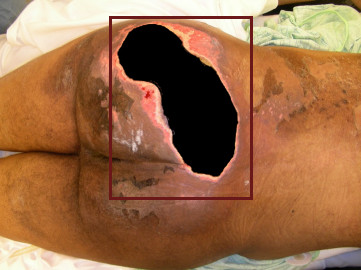
\includegraphics[keepaspectratio, width=3cm]{SourceCode/dataset/luka_hitam/41.jpg}
		\caption{Luka Hitam di-\textit{crop}}
	\end{subfigure}
	\begin{subfigure}{.3\textwidth}
		\centering
		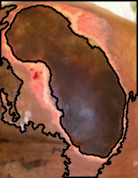
\includegraphics[keepaspectratio, width=3cm]{gambar/Bab3Extra/LukaHitamBorderFollowing.jpg}
		\caption{pindai luka hitam}
	\end{subfigure} 
	\begin{subfigure}{.3\textwidth}
		\centering
		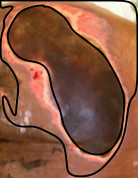
\includegraphics[keepaspectratio, width=3cm]{gambar/Bab3Extra/LukaHitamCurve.jpg}
		\caption{Luka diinterpolasi}
	\end{subfigure}
	\caption{Hasil Interpolasi citra}
\end{figure}

Seperti di penelitian Rizki, untuk mendapatkan hasil yang lebih 
akurat, dilakukan anotasi terlebih dahulu sehingga mengurangi 
kemungkinan untuk mendapatkan \textit{image noise} atau penggarisan 
tidak perlu pada hasil pendeteksian luka. 

Untuk membuat program interpolasi ini, dibuat dulu variabel
yang diperlukan untuk menjalankan rumus utama. Variabel
yang pertama dicari adalah $\bar{u}$ atau disebut \textit{knot} menggunakan
rumus \textit{chord length} (\ref*{chordlength2}), yang dihitung dengan
memasukkan sejumlah koordinat, lalu dihitung setiap panjang antara koordinat.
Setelah mendapatkan semua panjangnya, lalu ditotalkan untuk menjadi pembagi
sehingga didapatkan $\bar{u}$ sesuai dengan jumlah koordinatnya.
\begin{algorithm}[H]
  \caption{\textit{Chord Length}}
  \begin{algorithmic}[1]
  \Require{\{$\textbf{Q}_k\},k = 0,\dots, n$}
  \Ensure{$\bar{u}$[$n$]}
  \Function{ChordLength}{$\textbf{Q}_k$[$n$]}
    \State {$\bar{u}$[$n$]}
    \State {$\bar{u} \gets$ 0}
    \State {d $\gets$ 0}
    \For{$i \gets 0$ to $n$} \Comment{search of d (total length)}
      \State length $\gets$ $|\textbf{Q}_k - \textbf{Q}_{k-1}|$
      \State $d \gets d +$ length
      \State $\bar{u}$[$i$] $\gets d$
    \EndFor
    \For{$i \gets 0$ to $n$} \Comment{search of knots}
      \State $\bar{u}$[$i$] $\gets$ $\bar{u}$[$i$] $/ d$
    \EndFor
    \State \Return $\bar{u}$[$n$]
  \EndFunction
  \end{algorithmic}
  \label{algoritma:chordlength}
\end{algorithm}
\begin{itemize}
  \setlength{\itemsep}{0pt}
  \setlength{\parskip}{0pt}
  \setlength{\parsep}{0pt}
  \item $\{\textbf{Q}_k\}$ meurpakan input koordinat
  \item $k$ adalah indeks dari koordinat
  \item $n$ jumlah koordinat yang dimasukkan
  \item $\bar{u}$ \textit{knot}, hasil dari algoritma
\end{itemize}

Dari algoritma (\ref{algoritma:chordlength}), didapatkan array 
yang berisikan $\bar{u}$. Variabel selanjutnya adalah $U$ yang 
disebut juga \textit{knot vector} menggunakan rumus rata-rata 
knot (\ref*{penjarakanrata_rataknots}). Dimulai dengan mengambil
hasil dari algoritma {\ref{algoritma:chordlength}} lalu isi array
dengan indeks dari 0 sampai sederajatnya menjadi 0 dan mengisi
array dengan indeks setelah jumlah indeks dikurangi derajat dengan
angka 1. Diantara dari 0 dan 1, diisi dengan menghitung jumlah knot
didalam indeks yang tidak diubah, lalu dibagi dengan derajatnya.
\begin{algorithm}[H]
  \caption{Rata-rata Knot}
  \begin{algorithmic}[1]
  \Require{$\bar{u}$[$n$] and $p$}
  \Ensure{$U$[$n + p + 1$]}
  \Function{KnotVector}{$\bar{u}$[$n$], $p$}
    \State {$U$[$n + p + 1$] }
    \For{$i$ $\gets$ 0 to $n$}
      \If{$i \leq p$}
        \State $U$[$i$] $\gets 0$
      \ElsIf{$i \geq n - p - 1$}
        \State $U$[$i$] $\gets 1$
      \Else
        \State $U$[$i$] $\gets 0$
        \For{$ii \gets i-p$ to $i$}
          \State $U$[$i$] $\gets$ $U$[$i$] + $\bar{u}$[$ii$]
        \EndFor
        \State $U$[$i$] = $U$[$i$] $/ p$
      \EndIf
    \EndFor
    \State \Return $U$[$n + p + 1$]
  \EndFunction
  \end{algorithmic}
  \label{algoritma:knotvektor}
\end{algorithm}
\begin{itemize}
  \setlength{\itemsep}{0pt}
  \setlength{\parskip}{0pt}
  \setlength{\parsep}{0pt}
  \item $\bar{u}$ \textit{knot} yang didapat dari 
  algoritma (\ref{algoritma:chordlength})
  \item $n$ jumlah \textit{knot}
  \item $p$ merupakan derajat interpolasi
  \item $U$ \textit{knot vector}, hasil dari algoritma(\ref{algoritma:knotvektor})
\end{itemize}

Setelah mendapat dua variabel penting yaitu $\bar{u}$
dan $U$, sudah bisa menjalankan rumus dasar (\ref*{rumusdasarN}).
Algoritma dimasukkan empat variabel, yaitu \textit{knot} yang didapatkan
dari algoritma (\ref{algoritma:chordlength}), indeks, derajat, dan
\textit{knot vector} dari algoritma (\ref{algoritma:knotvektor}).
Yang pertama diperiksa adalah apakah derajatnya merupakan nol.
apabila derajatnya nol maka akan diperiksa \textit{knotnya} melebihi 
atau sama dengan \textit{knot vector} pada indeksnya dan kurang 
dari \textit{knot vector} dengan indeks selanjutnya. apabila
iya akan diberika angka satu, apabila tidak akan diberikan nol.
Selain dari derajat nol, maka algoritma ini akan menjadi rekursif
di mana akan selalu memanggil hasil dari derajat sebelumnya.
\begin{algorithm}[H]
  \caption{Rumus Dasar Spline (\textit{B-Spline})}
  \begin{algorithmic}[1]
  \Require{$\bar{u}$, $i$, $p$, $U$[\;]}
  \Ensure{spline}
  \Function{Spline}{$\bar{u}$, $i$, $p$, $U$[\;]}
    \If{$p$ is 0}
      \If{$U$[$i$] $\leq$ $\bar{u}$ < $U$[$i$+1]}
        \State \Return 1
      \Else
        \State \Return 0
      \EndIf
    \Else \Comment{separate left and right equation}
      \State left $\gets$ ($\bar{u}$ - $U$[$i$]) $/$ ($U$[$i+p$] - $U$[$i$])
      \State right $\gets$ ($U$[$i+p+1$] - $\bar{u}$) $/$ ($U$[$i+p+1$] - $U$[$i+1$])
      \State left $\gets$ left * Spline($\bar{u}$, $i$, $p-1$, $U$[\;]) \Comment{recursive}
      \State left $\gets$ right * Spline($\bar{u}$, $i+1$, $p-1$, $U$[\;])
      \State \Return left + right
    \EndIf
  \EndFunction
  \end{algorithmic}
  \label{algoritma:spline}
\end{algorithm}
\begin{itemize}
  \setlength{\itemsep}{0pt}
  \setlength{\parskip}{0pt}
  \setlength{\parsep}{0pt}
  \item $\bar{u}$ \textit{knot} yang didapat dari 
  algoritma (\ref{algoritma:chordlength})
  \item $i$ indeks yang akan dipakai pada algoritma(\ref{algoritma:globalinterpolation})
  \item $p$ merupakan derajat interpolasi
  \item $U$ \textit{knot vector}, didapat dari algoritma(\ref{algoritma:knotvektor})
\end{itemize}

Sebelum langkah terakhir adalah membuat matriks dari rumus (\ref{rumus:Global})
memanggil algoritma (\ref{algoritma:chordlength}), (\ref{algoritma:knotvektor}), 
dan (\ref{algoritma:spline}) yang lalu di \textit{inverse}-nya 
dikalikan dengan koordinat input.
\begin{algorithm}[H]
  \caption{\textit{Global Interpolation}}
  \begin{algorithmic}[1]
  \Require{\{$\textbf{Q}_k\},k = 0,\dots,n$, $p$}
  \Ensure{Curve Points}
  \Function{GlobalInterpolation}{$\textbf{Q}_k$[$n$], $p$}
    \State {$\bar{u}$ $\gets$ ChordLength($\textbf{Q}_k$[$n$])}
    \State {$U$ $\gets$ KnotVector($\bar{u}$, $p$)}
    \State {$\textit{C}$[$n_x$, $n_y$]}
    \For {$y$ $\gets$ 0 to $n_y$}
      \For {$x$ $\gets$ 0 to $n_x$}
        \State $\textit{C}$[$x,y$] = Spline($\bar{u}$[$x$], $y$, $p$, $U$)
      \EndFor
    \EndFor
  \State $\textit{C}$ $\gets$ Inverse$\_$of$\_$$\textit{C}$ * $\textbf{Q}$
  \State \Return $\textit{C}$
  \EndFunction
  \end{algorithmic}
  \label{algoritma:globalinterpolation}
\end{algorithm}

Langkah terakhir yang akan dilakukan dengan proses interpolasi 
adalah dengan membuat garis halus sesuai dengan titik-titik 
yang sudah dibuat oleh \textit{global interpolation}(\ref{algoritma:globalinterpolation}) 
menggunakan algoritma Bézier(\ref{kurvabezier})
\begin{algorithm}[H]
  \caption{\textit{Bézier}}
  \begin{algorithmic}
  \Require{CurvePoints, TotalPoints} \Comment{TotalPoints is how smooth the curve is}
  \Ensure{Curve}
  \Function{Bernstein}{$n, k, t$}
    \State \Return {binom($n ,k$) * $t^k$ * (1-$t$)$^{n-k}$} \Comment{binom function from scipy}
  \EndFunction
  \Function{Bezier}{CurvePoints, TotalPoints}
    \State {$N$ $\gets$ Length of CurvePoints}
    \State {$t$ $\gets$ sequence of numbers from 0 to 1 with the length of TotalPoints}
    \State {Curve $\gets$ [$\;$]}
    \For {$i \gets$ 0 to $N$}
      \State {Curve $\gets$ Bernstein($N$ - 1, $i, t$) * CurvePoints[$i$]}
    \EndFor
    \State \Return Curve
    \EndFunction
  \end{algorithmic}
  \label{algoritma:bezier}
\end{algorithm}


\section{Perancangan Eksperimen}

Pada subbab ini akan membahas bagaimana rancangan eksperimen
yang akan dilakukan dalam penelitian ini. Eksperimen dimulai
dengan pengolahan data, kemudian deteksi luka oleh sistem
yang diakhiri dengan validasi data.

\subsection{Sumber Data}

Dikarenakan penulis melanjutkan penelitian dari Rizki, maka
penulis akan menggunakan sumber data yang sama, yaitu bersumber
dari penelitian luka Ns. Ratna Aryani, M.Kep, tahun 2018 
(\cite{Aryani:2018}) diambil dari data klinik yang tersedia di \href{https://github.com/mekas/InjuryDetection}
{https://github.com/mekas/InjuryDetection}, berjumlahkan 108 luka. dari sumber tersebut, 
terdapat 37 data yang tidak dapat dipakai karena data tersebut
merupakan duplikat dari sumber yang sama sehingga data yang
dipakai berjumlah 69 buah citra. Dari citra tersebut, terdapat
24 luka hitam, 15 luka kuning, dan 30 luka merah.
\begin{figure}[H]
	\centering
	\begin{subfigure}{.3\textwidth}
		\centering
		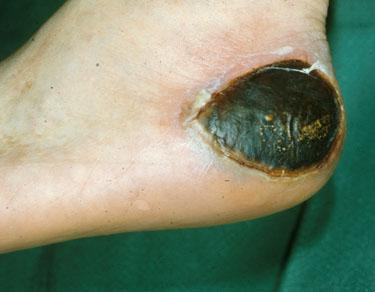
\includegraphics[keepaspectratio, width=3cm]{gambar/Bab3Extra/LukaHitam.jpg}
		\caption{Luka Hitam}
	\end{subfigure}
	\begin{subfigure}{.3\textwidth}
		\centering
		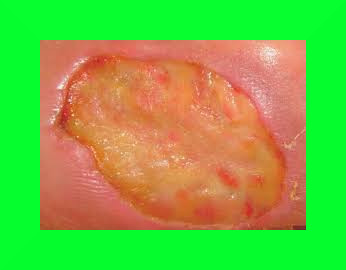
\includegraphics[keepaspectratio, width=3cm]{gambar/Bab3Extra/LukaKuning.jpg}
		\caption{Luka Kuning}
	\end{subfigure} 
	\begin{subfigure}{.3\textwidth}
		\centering
		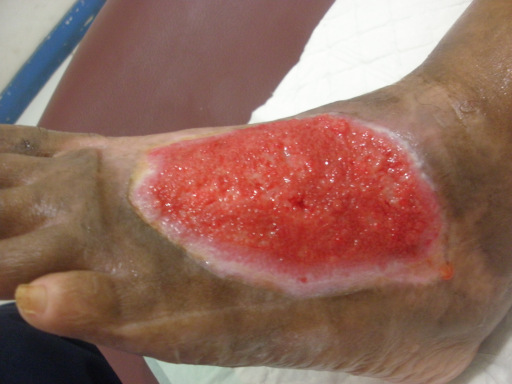
\includegraphics[keepaspectratio, width=3cm]{gambar/Bab3Extra/LukaMerah.jpg}
		\caption{Luka Merah}
	\end{subfigure}
	\caption{Data citra luka}
\end{figure}

\subsection{Validasi}

Seperti pada penelitian Rizki, akan diperiksa dahulu apakah hasil
pindai berhasil atau tidak. Setelah mendapatkan 
hasil deteksi keliling luka, harus divalidasi
ketepatan alat deteksi tersebut. penulis akan memvalidasi
data deteksi dengan menghitung selisih piksel dari hasil
alat deteksi, dengan \textit{ground truth} yang diambil dari
gambar manual menggunakan program GIMP.
similaritas akan dihitung sebagai berikut

\begin{equation}
  similiaritas(\%) = 100 - \left| \frac{luas \; ground \; truth - luas \; hasil \; deteksi}
  {luas \; ground \; truth} * 100  \right|
  \label{rumus:groundtruth}
\end{equation}

\begin{figure}[H]
	\centering
	\begin{subfigure}{.3\textwidth}
		\centering
		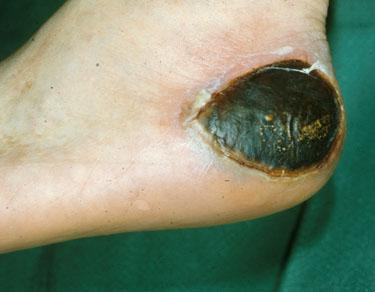
\includegraphics[keepaspectratio, width=3cm]{gambar/Bab3Extra/LukaHitam.jpg}
		\caption{Luka Hitam}
	\end{subfigure}
	\begin{subfigure}{.3\textwidth}
		\centering
		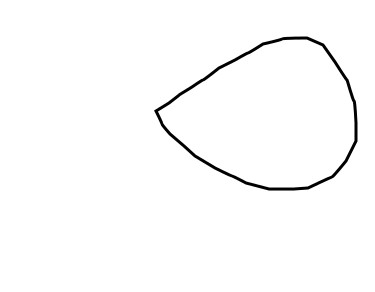
\includegraphics[keepaspectratio, width=3cm]{gambar/Bab3Extra/LukaHitamManual.jpg}
		\caption{Gambar Manual}
	\end{subfigure} 
	\begin{subfigure}{.3\textwidth}
		\centering
		
\includegraphics[keepaspectratio, width=3cm]{gambar/Bab3Extra/LukaHitamInt.jpg}
		\caption{Deteksi Interpolasi milik Rizki}
	\end{subfigure}
	\caption{Validasi alat deteksi}
\end{figure}

% Baris ini digunakan untuk membantu dalam melakukan sitasi
% Karena diapit dengan comment, maka baris ini akan diabaikan
% oleh compiler LaTeX.
\begin{comment}
  \bibliography{daftar-pustaka}
\end{comment}
%!TEX root = ./template-skripsi.tex
%-------------------------------------------------------------------------------
%                            	BAB IV
%               		KESIMPULAN DAN SARAN
%-------------------------------------------------------------------------------

\chapter{HASIL DAN PEMBAHASAN}

\section{Pengolahan data citra input}

Untuk optimal nya pendeteksia luka, maka piksel 
yang dipindai dikurangi dengan memotong citra yang 
dipindai. Pemotongan ini dilakukan dengan menggunakan 
program GIMP(\textit{GNU Image Manipulation Program}) dan 
memakai fungsi \textit{crop} 

Langkah selanjutnya dalam pengolahan citra ini dimulai dengan 
membaca citra nya dalam bentuk hitam putih(\textit{grayscale}). 
Proses pengolahan data citra input menggunakan \textit{imread} yang merupakan 
fungsi yang di-\textit{import} dari CV2
\begin{figure}[H]
	\centering
	\begin{lstlisting}[language=Python, basicstyle=\tiny]
		import cv2 as cv2

		gambar = cv2.imread(image, cv2.IMREADGRAYSCALE)
	\end{lstlisting}
	\caption{Kode untuk membaca citra}
	\label{kode:imread}
\end{figure}

\section{Deteksi Keliling Menggunakan \textit{Border Following}}

Citra yang sudah dimasukkan akan diolah oleh program 
\textit{border following}. Metode ini akan membaca citra 
dalam bentuk citra biner yang hanya terisi 0 dan 1. 
Dibentuklah kode sebagai berikut yang mengikuti kode 
dibuat oleh Hafizhun Alim(\cite{Hafizhun}) pada skripsi-nya 
yang berjudul "\textit{Fish Movement Tracking Menggunakan 
Metode Gaussian Mixture Models (GMM) dan Kalman Filter}".
\begin{figure}[H]
	\centering
	\begin{lstlisting}[language=Python, basicstyle=\tiny]
		def border_following(self, img, start, previous):

			pointer_one = previous
			pointer_three = start
			contour = []

		# Step 3.1 Move clockwise
		count = 0
		while img[pointer_one[0]][pointer_one[1]] == 0:
			# If the starting pixel is a single pixel dot
			if count > 7:
				img[pointer_three[0]][pointer_three[1]] = 4
				contour.append(np.array([[pointer_three[1] - 1, pointer_three[0] - 1]]))
				return np.array(contour)
					
			position, next_pointer = self.next_pointer_position(pointer_one, pointer_three, 1)
			pointer_one = next_pointer
			count += 1
	
	\end{lstlisting}
\end{figure}
\begin{figure}[H]
	\centering
	\begin{lstlisting}[language=Python, basicstyle=\tiny]
        # Step 3.2
        pointer_two = copy.copy(pointer_one)

        counter = 0
        while True:
            # Step 3.3 Move counter clockwise
            # First, move pointer one time in counter-clockwise direction
            position, next_pointer = self.next_pointer_position(pointer_two, pointer_three, 2)
            pointer_two = next_pointer
            while img[pointer_two[0]][pointer_two[1]] == 0:
                position, next_pointer = self.next_pointer_position(pointer_two, pointer_three, 2)
                pointer_two = next_pointer
            pointer_four = pointer_two
			
		# Step 3.4 Assign NBD
		# rows or i represent y-axis
		# cols or j represent x-axis
		# the coordinate are inverted because we wanted to return a set of (x, y) points, not (y, x)
		# we use 2 and 4 (-2) since we only extract outer border
		nbd_coordinate = copy.copy(pointer_three)
		if img[nbd_coordinate[0]][nbd_coordinate[1] + 1] == 0:
			img[nbd_coordinate[0]][nbd_coordinate[1]] = 4
		elif img[nbd_coordinate[0]][nbd_coordinate[1] + 1] != 0 and img[nbd_coordinate[0]][nbd_coordinate[1]] == 1:
			img[nbd_coordinate[0]][nbd_coordinate[1]] = 2
            contour.append(np.array([[nbd_coordinate[1] - 1, nbd_coordinate[0] - 1]]))

            # Step 3.5 Determine new pointer or break
            if pointer_four[0] == start[0] and pointer_four[1] == start[1]:
                if pointer_three[0] == pointer_one[0] and pointer_three[1] == pointer_one[1]:
                    break
            pointer_two = copy.copy(pointer_three)
            pointer_three = copy.copy(pointer_four)

            counter += 1

        return np.array(contour)
	\end{lstlisting}
	\caption{Kode border following}
	\label{kode:border following}
\end{figure}

setelah jalannya program diatas, didapatkan 
hasil contour sebagai berikut
\begin{figure}[H]
	\centering
	\begin{subfigure}{.3\textwidth}
		\centering
		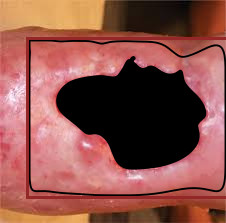
\includegraphics[keepaspectratio, width=3cm]{SourceCode/dataset/luka_merah/33.jpg}
		\caption{Sumber citra}
	\end{subfigure}
	\begin{subfigure}{.4\textwidth}
		\centering
		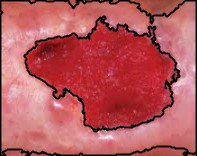
\includegraphics[keepaspectratio, width=3cm]{gambar/Bab4/Luka_merah_interpolasi.jpg}
		\caption{Hasil \textit{border following}}
	\end{subfigure} 
	\caption{Hasil pindai \textit{border following}}
\end{figure}
Dalam pendeteksiannya, metode ini akan menghasilkan 
lebih dari daerah dan terkadang mendeteksi daerah 
yang hanya memiliki satu titik koordinat. Untuk membuang 
daerah yang pasti bukan daerah luka, maka penulis 
hanya menggambar daerah yang memiliki 50 titik.


\section{Penghalusan menggunakan Interpolasi Global}

Dari hasil \textit{border following}, akurasi dari 
pindaian citra masih kasar dan belum 100$\%$ kepada 
\textit{ground truth}. Untuk membantu ini, penulis 
menggunakan \textit{Global Interpolation} yang ada 
di buku NURBS(\cite{PiegTill96}).

Penulis tidak menggunakan interpolasi lokal dikarenakan 
kurang mampunya penulis untuk mengerti cara penghitungan 
interpolasi lokal. Banya variabel yang penulis kurang tangkap 
seperti pada rumus(\ref{rumus:localbicubic}), di mana memiliki 
dua jenis \textit{knot vector} yang penulis tidak tahu 
perbedaannya.

Dimulai dengan rumus utama akan menggunakan 
algoritma(\ref{algoritma:globalinterpolation}). 
Algoritma ini akan membentuk kode sebagai berikut
\begin{figure}[H]
	\centering
	\begin{lstlisting}[language=Python, basicstyle=\tiny]
		def GlobalCurveInterpolation(Point, degree):
			Knot = GlobalInterpolation.ChordLength(Point)
			KnotVector = GlobalInterpolation.knotGlobalCurve(Knot, degree)
			nurb = np.empty([len(Point), len(Point)])
			for x in range(len(Point)):
				for y in range(len(Point)):
					nurb[x,y] = GlobalInterpolation.N(Knot[x], y, degree, KnotVector)

			#making sure the last array
			nurb[len(Point)-1,len(Point)-1] = 1.0

		
			hasil = np.dot(np.linalg.pinv(nurb), Point)

			return hasil
	\end{lstlisting}
	\caption{Kode Global Interpolation}
	\label{kode:GlobalInterpolation}
\end{figure}
Dari kode di atas, terdapat beberapa fungsi 
dari \textit{class} GlobalInterpolation yang 
akan dijelaskan sebagai berikut

Dalam interpolasi, menentukan titik-titik kurva 
membutuhkan \textit{knot}. \textit{Knot} dapat 
ditentukan dengan perata-rataan memakai fungsi 
\textit{numpy} yaitu np.linspace(0,1,len(Point)).
Ada juga metode lain yang memastikan kurva lebih 
stabil yaitu menggunakan \textit{chord length} 
menggunakan algoritma(\ref{algoritma:chordlength}).
\begin{figure}[H]
	\centering
	\begin{lstlisting}[language=Python, basicstyle=\tiny]
		def ChordLength(koordinat = np.array([0,0])):
			knot = np.empty([len(koordinat)],dtype=float)
			knot[0] = 0
			totalJarak = 0

			#d / total jarak
			for i in range(len(koordinat)):
				if(i>0):
					jarak = np.linalg.norm(koordinat[i-1] - koordinat[i])
					totalJarak += jarak
					knot[i] = totalJarak
		
			#knotkord
			for i in range(len(koordinat)):
				knot[i] = knot[i]/totalJarak

			#return as KnotVector, group of knots, 1d array
        	return np.array(knot)
	\end{lstlisting}
	\caption{Kode \textit{chord length}}
	\label{kode:chordlength}
\end{figure}

Setelah mendapatkan knot, langkah selanjutnya 
adalah membuat \textit{knot vector}. Kode untuk 
\textit{knot vector} akan dibentuk mengikuti 
algoritma(\ref{algoritma:knotvektor})
\begin{figure}[H]
	\centering
	\begin{lstlisting}[language=Python, basicstyle=\tiny]
		def knotGlobalCurve(knots = np.array([0]), degree=0):

			KnotVector = np.empty([len(knots) + degree + 1])
			for i, val in enumerate(KnotVector):
				if(i <= degree): KnotVector[i] = 0 
				elif(i >= len(KnotVector) - degree-1): KnotVector[i] = 1
				else:
					knotvector = 0.0
					for ii in range(i-degree, i):
						knotvector += knots[ii]
					KnotVector[i] = knotvector/degree

			#return as 1d array
			return KnotVector
	\end{lstlisting}
	\caption{Kode knot vector}
	\label{kode:knotvector}
\end{figure}

Dan metode utama yang dijalankan secara rekursif, 
yaitu rumus dasar interpolasi yang dilambangkan 
sebagai N di buku \textit{NURBS}. Dalam pembuatannya, 
penulis agak kesulitan dalam mendapatkan hasil yang 
ditujukan oleh buku. Masalah yang pertama dihadapi 
adalah membuat 0/0 menjadi 0. yang penulis pertama 
kali lakukan adalah mengecek penyebut merupakan 0 maka 
hasilnya akan 0. Metode ini menghasilkan nilai yang salah 
pada baris awal dan terakhir dan membuat kolom tengah 
menjadi 1 semua. Lalu, karena penyebut terjadi operasi 
pengurangan, pengecek nya diubah dengan apabila variabel 
kiri sama dengan yang kanan. Setelah pengetesan hampir 
semua nya benar kecuali angka terakhir, yang seharusnya 1 
menjadi 0, di sini penulis memaksa angka matriks terakhir 
menjadi 1. Berikut adalah kode untuk rumus dasar mengikuti
algoritma(\ref{algoritma:spline}).
\begin{figure}[H]
	\centering
	\begin{lstlisting}[language=Python, basicstyle=\tiny]
		def N(knot = 0.0, i = 0 , degree = 0, KnotVector = np.array([0])):

			#Basis function that used to count N in interpolation

			if (degree == 0):
				#
				return 1.0 if (KnotVector[i] <= knot < KnotVector[i + 1]) else 0.0
			else:
				
				#count the left side and right side of equation
				kiri = 0.0 if(KnotVector[i + degree] == KnotVector[i]) else (knot - KnotVector[i]) / (KnotVector[i + degree] - KnotVector[i]) * GlobalInterpolation.N(knot, i, degree - 1, KnotVector)
				kanan = 0.0 if(KnotVector[i + degree + 1] == KnotVector[i + 1]) else (KnotVector[i + degree + 1] - knot) / (KnotVector[i + degree + 1] - KnotVector[i + 1]) * GlobalInterpolation.N(knot, i + 1, degree - 1, KnotVector)
			
				return kiri + kanan
	\end{lstlisting}
	\caption{Kode rumus dasar (N)}
	\label{kode:rumusdasar}
\end{figure}

Dari semua kode di atas, sudah bisa dijalankan 
sebagai satu program yang akan menghasilkan citra 
dengan input dari \textit{border following}
\begin{figure}[H]
	\centering
	\begin{subfigure}{.3\textwidth}
		\centering
		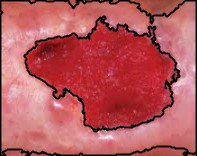
\includegraphics[keepaspectratio, width=3cm]{gambar/Bab4/Luka_merah_interpolasi.jpg}
		\caption{\textit{Border following}}
	\end{subfigure}
	\begin{subfigure}{.4\textwidth}
		\centering
		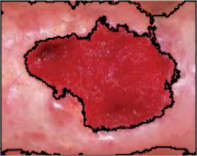
\includegraphics[keepaspectratio, width=3cm]{gambar/Bab4/Luka_merah_Globalinterpolasi.jpg}
		\caption{Hasil interpolasi}
	\end{subfigure} 
	\caption{Hasil Interpolasi dari deteksi \textit{border following}}
\end{figure}

Dari metode yang dipakai di atas, hanya didapatkan 
titik kontrol dari suatu kurva. Untuk mendapatkan 
kurva halus seperti yang dicanangkan dalam buku 
yang akan menghasilkan gambar(\ref{gambar:kurvaluka})
\textit{NURBS} dipakai algoritma dari Bézier(\ref{algoritma:bezier})
\begin{figure}[H]
	\centering
	\begin{lstlisting}[language=Python, basicstyle=\tiny]
		bernstein = lambda n, k, t: binom(n,k)* t**k * (1.-t)**(n-k)

		def bezier(points, num=400):
			N = len(points)
			t = np.linspace(0, 1, num=num)
			curve = np.zeros((num, 2))
			for i in range(N):
				curve += np.outer(GlobalInterpolation.bernstein(N - 1, i, t), points[i])
			return curve
	\end{lstlisting}
	\caption{Kode Bézier}
	\label{kode:bezier}
\end{figure}
\begin{figure}[H]
	\centering
	\begin{subfigure}{.3\textwidth}
		\centering
		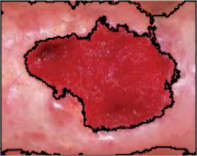
\includegraphics[keepaspectratio, width=3cm]{gambar/Bab4/Luka_merah_Globalinterpolasi.jpg}
		\caption{Interpolasi global}
	\end{subfigure}
	\begin{subfigure}{.4\textwidth}
		\centering
		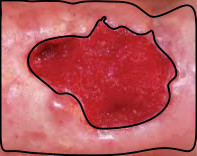
\includegraphics[keepaspectratio, width=3cm]{gambar/Bab4/Luka_merah_curve.jpg}
		\caption{Kurva bézier}
	\end{subfigure} 
	\caption{Penghalusan kurva menggunakan bézier}
	\label{gambar:kurvaluka}
\end{figure}
Kekurangan dari kode ini adalah kode ini tidak bisa diberi 
titik data yang banyak, sehingga penulis membataskan titik data 
menjadi 1000 dengan memotong titik data secara rata.

\section{Validasi}

Source image eksperimen diambil dari repository yang dapat diakses di
\href{https://github.com/mekas/InjuryDetection}{https://github.com/mekas/InjuryDetection}. 
Dari semua metode yang sudah ditunjukan 
dalam bab ini, maka akan dijalankan ke semua citra yang 
berada dalam repository. 

Dalam pengolahan citra, tidak semua citra dapat dipindai 
dengan baik. Apabila suatu pindaian dekat dengan bentuk 
\textit{ground truth} maka akan dikategorikan sebagai 
berhasil dan yang sebaliknya akan dikategorikan sebagai 
gagal seperti yang ditunjukan pada gambar(\ref{suksesgagal}). 
Hasil dari pindaian akan dimasukkan kedalam lampiran.
\begin{figure}[H]
	\centering
	\begin{subfigure}{.3\textwidth}
		\centering
		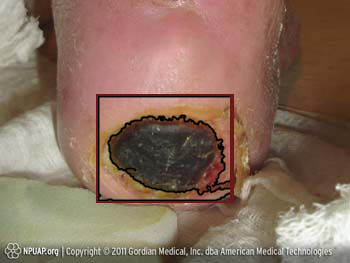
\includegraphics[keepaspectratio, width=3cm]{gambar/Data/BorderFollowing/Hitam/6 - failed.jpg}
		\caption{Gagal}
	\end{subfigure}
	\begin{subfigure}{.4\textwidth}
		\centering
		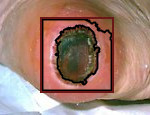
\includegraphics[keepaspectratio, width=3cm]{gambar/Data/BorderFollowing/Hitam/7 - sukses.jpg}
		\caption{Berhasil}
	\end{subfigure} 
	\caption{Alat validasi}
	\label{suksesgagal}
\end{figure}

Dalam memvalidasi citra, akan digunakan 
\textit{GIMP} dengan menggunakan \textit{fuzzy select tool} 
dengan treshold 75.- dan 2px feather edges lalu dilihat 
\textit{pixel count} nya dengan menggunakan \textit{histogram}. 
Karena program yang penulis pakai hanya memberi garis luar, maka 
daerah yang terdeteksi akan dihitamkan manual agar dapat 
dihitung luasnya. Setelah mendapatkan luas dari sumber data, 
maka akan dibandingkan dengan \textit{ground truth} menggunakan 
rumus(\ref{rumus:groundtruth})
\begin{figure}[H]
	\centering
	\begin{subfigure}{.3\textwidth}
		\centering
		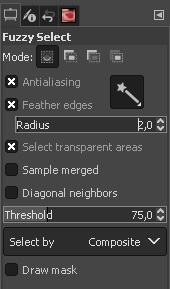
\includegraphics[keepaspectratio, width=3cm]{gambar/Bab4/fuzzyselect.jpg}
		\caption{\textit{fuzzyselect tool}}
	\end{subfigure}
	\begin{subfigure}{.4\textwidth}
		\centering
		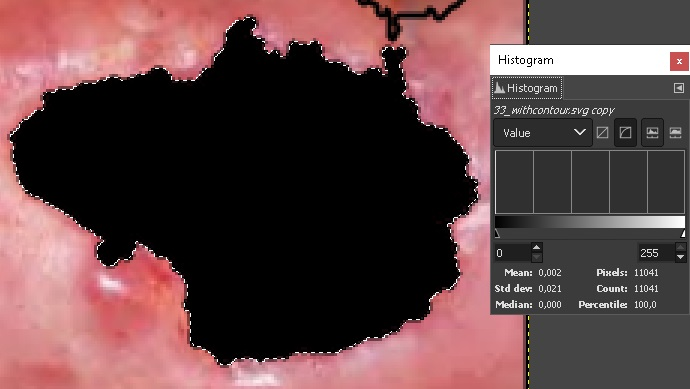
\includegraphics[keepaspectratio, width=3cm]{gambar/Bab4/histogram.jpg}
		\caption{\textit{histogram}}
	\end{subfigure} 
	\caption{Alat validasi}
\end{figure}

Percobaan dimulai dengan luka merah, didapatkan hasil sebagai berikut.
\begin{longtable}[width = 8cm]{| c | c | c | c | c |}
	\caption{Percobaan pada luka merah}
	\\
	\hline
	Indeks & Sumber & \textit{Border Following} & Interpolasi & \textit{Ground Truth}
	\endhead
	\hline\hline
	\multicolumn{5}{|c|}
	{Luka Merah}
	\\
	\hline\hline
	12 &
    \includegraphics[keepaspectratio, width=2cm]
    {Skripkating/Rizki_Wound_ACM/dataset_3/luka_merah/ready/12.jpg} &
    \includegraphics[keepaspectratio, width=2cm]
    {gambar/Data/BorderFollowing/Merah/12.jpg} &
    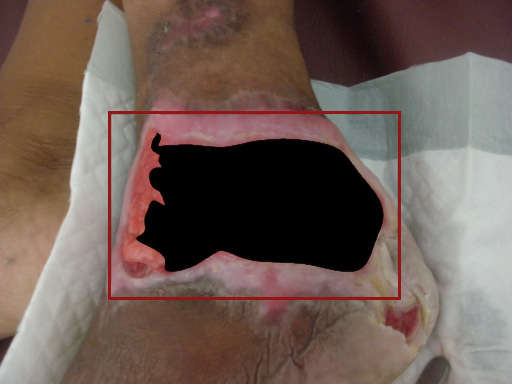
\includegraphics[keepaspectratio, width=2cm]
    {gambar/Data/Curve/Merah/12.jpg} &
    \includegraphics[keepaspectratio, width=2cm]
    {Skripkating/Rizki_Wound_ACM/dataset_3/luka_merah/ready/12_r.jpg}
	\\
	\hline
	18 &
    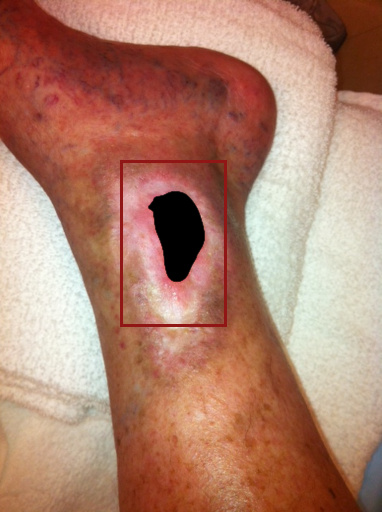
\includegraphics[keepaspectratio, width=2cm]
    {Skripkating/Rizki_Wound_ACM/dataset_3/luka_merah/ready/18.jpg} &
    \includegraphics[keepaspectratio, width=2cm]
    {gambar/Data/BorderFollowing/Merah/18.jpg} &
    \includegraphics[keepaspectratio, width=2cm]
    {gambar/Data/Curve/Merah/18.jpg} &
    \includegraphics[keepaspectratio, width=2cm]
    {Skripkating/Rizki_Wound_ACM/dataset_3/luka_merah/ready/18_r.jpg}
	\\
	\hline
	33 &
    \includegraphics[keepaspectratio, width=2cm]
    {Skripkating/Rizki_Wound_ACM/dataset_3/luka_merah/ready/33.jpg} &
    \includegraphics[keepaspectratio, width=2cm]
    {gambar/Data/BorderFollowing/Merah/33.jpg} &
    \includegraphics[keepaspectratio, width=2cm]
    {gambar/Data/Curve/Merah/33.jpg} &
    \includegraphics[keepaspectratio, width=2cm]
    {Skripkating/Rizki_Wound_ACM/dataset_3/luka_merah/ready/33_r.jpg}
	\\
	\hline
	44 &
    \includegraphics[keepaspectratio, width=2cm]
    {Skripkating/Rizki_Wound_ACM/dataset_3/luka_merah/ready/44.jpg} &
    \includegraphics[keepaspectratio, width=2cm]
    {gambar/Data/BorderFollowing/Merah/44.jpg} &
    \includegraphics[keepaspectratio, width=2cm]
    {gambar/Data/Curve/Merah/44.jpg} &
    \includegraphics[keepaspectratio, width=2cm]
    {Skripkating/Rizki_Wound_ACM/dataset_3/luka_merah/ready/44_r.jpg}
	\\
	\hline
\end{longtable}
\begin{longtable}[width = 6cm]{| c | c | c | c | c | c |}
    \caption{Similiaritas deteksi luka merah \textit{border following} 
    dan yang dibantu dengan interpolasi}
    \\
    \hline  
    \multicolumn{6}{|c|}{Luka Merah}
    \\
    \hline
    Indeks & \textbf{GT}(px) & \textbf{BF}(px) & Similiaritas($\%$) & Intp(px) & Similiaritas($\%$)
    \endhead
    \hline  12&	29834&	26565&	89.04270296&	26182&	87.75893276 \\
    \hline  18&	2788&	3596&	71.01865136&	3337&	80.30846485 \\
    \hline  33&	10951&	11176&	97.94539311&	10732&	98.00018263 \\
    \hline  44&	2395&	4172&	25.80375783&	3966&	34.40501044 \\
    \hline  \multicolumn{2}{|c|}{}& \textit{Average}&    70.95262632&    \textit{Average}&    75.11814767 \\
    \hline
\end{longtable}
\begin{itemize}
    \setlength{\itemsep}{0pt}
    \setlength{\parskip}{0pt}
    \setlength{\parsep}{0pt}
    \item GT = \textit{Ground Truth}
    \item BF = \textit{Border Following}
    \item Intp = Interpolasi
\end{itemize}
\begin{itemize}
    \setlength{\itemsep}{0pt}
    \setlength{\parskip}{0pt}
    \setlength{\parsep}{0pt}
    \item Jumlah luka merah = 30
    \item Jumlah luka yang terdeteksi contour tracing = 4
\end{itemize}
Dari percobaan deteksi luka merah, tingkat pendeteksian 
dari \textit{border following} lumayan rendah, terdapat 4 
pindaian yang berhasil dari 30 citra, namun memiliki 
similiaritas yang bagus terhadap \textit{ground truth}, dan 
Bantuan dari Interpolasi meningkatkan similiaritas 
sebesar 4.16$\%$. 

Percobaan akan dilanjut ke luka kuning.
\begin{longtable}[width = 8cm]{| c | c | c | c | c |}
	\caption{Percobaan pada luka kuning}
	\\
	\hline
	Indeks & Sumber & \textit{Border Following} & Interpolasi & \textit{Ground Truth}
	\endhead
	\hline\hline
	\multicolumn{5}{|c|}
	{Luka Kuning}
	\\
	\hline\hline
	17 &
    \includegraphics[keepaspectratio, width=2cm]
    {Skripkating/Rizki_Wound_ACM/dataset_3/luka_kuning/ready/17.jpg} &
    \includegraphics[keepaspectratio, width=2cm]
    {gambar/Data/BorderFollowing/Kuning/17.jpg} &
    \includegraphics[keepaspectratio, width=2cm]
    {gambar/Data/Curve/Kuning/17.jpg} &
    \includegraphics[keepaspectratio, width=2cm]
    {Skripkating/Rizki_Wound_ACM/dataset_3/luka_kuning/ready/17_r.jpg}
	\\
	\hline
	25 &
    \includegraphics[keepaspectratio, width=2cm]
    {Skripkating/Rizki_Wound_ACM/dataset_3/luka_kuning/ready/25.jpg} &
    \includegraphics[keepaspectratio, width=2cm]
    {gambar/Data/BorderFollowing/Kuning/25.jpg} &
    \includegraphics[keepaspectratio, width=2cm]
    {gambar/Data/Curve/Kuning/25.jpg} &
    \includegraphics[keepaspectratio, width=2cm]
    {Skripkating/Rizki_Wound_ACM/dataset_3/luka_kuning/ready/25_r.jpg}
	\\
	\hline
\end{longtable}
\begin{longtable}[width = 6cm]{| c | c | c | c | c | c |}
    \caption{Similiaritas deteksi luka kuning \textit{border following} 
    dan yang dibantu dengan interpolasi}
    \\
    \hline  
    \multicolumn{6}{|c|}{Luka Kuning}
    \\
    \hline
    Indeks & \textbf{GT}(px) & \textbf{BF}(px) & Similiaritas($\%$) & Intp(px) & Similiaritas($\%$)
    \endhead
    \hline  17&	319&	317&	99.37304075&	282&	88.40125392 \\
    \hline  25&	2831&	1345&	47.50971388&	1291&	45.60226069 \\
    \hline  \multicolumn{2}{|c|}{}& \textit{Average}&    73.44137732&    \textit{Average}&    67.0017573 \\
    \hline
\end{longtable}
\begin{itemize}
    \setlength{\itemsep}{0pt}
    \setlength{\parskip}{0pt}
    \setlength{\parsep}{0pt}
    \item GT = \textit{Ground Truth}
    \item BF = \textit{Border Following}
    \item Intp = Interpolasi
\end{itemize}
\begin{itemize}
    \setlength{\itemsep}{0pt}
    \setlength{\parskip}{0pt}
    \setlength{\parsep}{0pt}
    \item Jumlah luka kuning = 15
    \item Jumlah luka yang terdeteksi contour tracing = 2
\end{itemize}
Setelah melakukan percobaan di luka kuning, dapat dilihat 
tingkat pendeteksian masih sama seperti pada luka merah, yaitu 
13.3$\%$, namun mendapat peningkatan pada pengecekan similiaritas 
di \textit{border following} pada angka 73.4$\%$, tetapi terjadi 
penurunan 6.43$\%$ di bantuan interpolasi terhadap \textit{border following}

Kategori terakhir untuk dipercobakan adalah luka hitam.
\begin{longtable}[width = 8cm]{| c | c | c | c | c |}
	\caption{Percobaan pada luka hitam}
	\\
	\hline
	Indeks & Sumber & \textit{Border Following} & Interpolasi & \textit{Ground Truth}
	\endhead
	\hline\hline
	\multicolumn{5}{|c|}
	{Luka Hitam}
	\\
	\hline\hline
	7 &
    \includegraphics[keepaspectratio, width=2cm]
    {Skripkating/Rizki_Wound_ACM/dataset_3/luka_hitam/ready/7.jpg} &
    \includegraphics[keepaspectratio, width=2cm]
    {gambar/Data/BorderFollowing/Hitam/7.jpg} &
    \includegraphics[keepaspectratio, width=2cm]
    {gambar/Data/Curve/Hitam/7.jpg} &
    \includegraphics[keepaspectratio, width=2cm]
    {Skripkating/Rizki_Wound_ACM/dataset_3/luka_hitam/ready/7_r.jpg}
	\\
	\hline
	18 &
    \includegraphics[keepaspectratio, width=2cm]
    {Skripkating/Rizki_Wound_ACM/dataset_3/luka_hitam/ready/18.jpg} &
    \includegraphics[keepaspectratio, width=2cm]
    {gambar/Data/BorderFollowing/Hitam/18.jpg} &
    \includegraphics[keepaspectratio, width=2cm]
    {gambar/Data/Curve/Hitam/18.jpg} &
    \includegraphics[keepaspectratio, width=2cm]
    {Skripkating/Rizki_Wound_ACM/dataset_3/luka_hitam/ready/18_r.jpg}
	\\
	\hline
	26 &
    \includegraphics[keepaspectratio, width=2cm]
    {Skripkating/Rizki_Wound_ACM/dataset_3/luka_hitam/ready/26.jpg} &
    \includegraphics[keepaspectratio, width=2cm]
    {gambar/Data/BorderFollowing/Hitam/26.jpg} &
    \includegraphics[keepaspectratio, width=2cm]
    {gambar/Data/Curve/Hitam/26.jpg} &
    \includegraphics[keepaspectratio, width=2cm]
    {Skripkating/Rizki_Wound_ACM/dataset_3/luka_hitam/ready/26_r.jpg}
	\\
	\hline
	28 &
    \includegraphics[keepaspectratio, width=2cm]
    {Skripkating/Rizki_Wound_ACM/dataset_3/luka_hitam/ready/28.jpg} &
    \includegraphics[keepaspectratio, width=2cm]
    {gambar/Data/BorderFollowing/Hitam/28.jpg} &
    \includegraphics[keepaspectratio, width=2cm]
    {gambar/Data/Curve/Hitam/28.jpg} &
    \includegraphics[keepaspectratio, width=2cm]
    {Skripkating/Rizki_Wound_ACM/dataset_3/luka_hitam/ready/28_r.jpg}
	\\
	\hline
	29 &
    \includegraphics[keepaspectratio, width=2cm]
    {Skripkating/Rizki_Wound_ACM/dataset_3/luka_hitam/ready/29.jpg} &
    \includegraphics[keepaspectratio, width=2cm]
    {gambar/Data/BorderFollowing/Hitam/29.jpg} &
    \includegraphics[keepaspectratio, width=2cm]
    {gambar/Data/Curve/Hitam/29.jpg} &
    \includegraphics[keepaspectratio, width=2cm]
    {Skripkating/Rizki_Wound_ACM/dataset_3/luka_hitam/ready/29_r.jpg}
	\\
	\hline
	33 &
    \includegraphics[keepaspectratio, width=2cm]
    {Skripkating/Rizki_Wound_ACM/dataset_3/luka_hitam/ready/33.jpg} &
    \includegraphics[keepaspectratio, width=2cm]
    {gambar/Data/BorderFollowing/Hitam/33.jpg} &
    \includegraphics[keepaspectratio, width=2cm]
    {gambar/Data/Curve/Hitam/33.jpg} &
    \includegraphics[keepaspectratio, width=2cm]
    {Skripkating/Rizki_Wound_ACM/dataset_3/luka_hitam/ready/33_r.jpg}
	\\
	\hline
	40 &
    \includegraphics[keepaspectratio, width=2cm]
    {Skripkating/Rizki_Wound_ACM/dataset_3/luka_hitam/ready/40.jpg} &
    \includegraphics[keepaspectratio, width=2cm]
    {gambar/Data/BorderFollowing/Hitam/40.jpg} &
    \includegraphics[keepaspectratio, width=2cm]
    {gambar/Data/Curve/Hitam/40.jpg} &
    \includegraphics[keepaspectratio, width=2cm]
    {Skripkating/Rizki_Wound_ACM/dataset_3/luka_hitam/ready/40_r.jpg}
	\\
	\hline
	41 &
    \includegraphics[keepaspectratio, width=2cm]
    {Skripkating/Rizki_Wound_ACM/dataset_3/luka_hitam/ready/41.jpg} &
    \includegraphics[keepaspectratio, width=2cm]
    {gambar/Data/BorderFollowing/Hitam/41.jpg} &
    \includegraphics[keepaspectratio, width=2cm]
    {gambar/Data/Curve/Hitam/41.jpg} &
    \includegraphics[keepaspectratio, width=2cm]
    {Skripkating/Rizki_Wound_ACM/dataset_3/luka_hitam/ready/41_r.jpg}
	\\
	\hline
\end{longtable}
\begin{longtable}[width = 6cm]{| c | c | c | c | c | c |}
    \caption{Similiaritas deteksi luka hitam \textit{border following} 
    dan yang dibantu dengan interpolasi}
    \\
    \hline  
    \multicolumn{6}{|c|}{Luka Hitam}
    \\
    \hline
    Indeks & \textbf{GT}(px) & \textbf{BF}(px) & Similiaritas($\%$) & Intp(px) & Similiaritas($\%$)
    \endhead
    \hline  7&	2146&	2061&	96.03914259&	1928&	89.8415657  \\
    \hline  18&	7328&	6430&	87.74563319&	6009&	82.00054585 \\
    \hline  26&	60411&	60923&	99.15247223&	59143&	97.90104451 \\
    \hline  28&	5408&	5608&	96.30177515&	5902&	90.86538462 \\
    \hline  29&	43763&	44984&	97.20997189&	43368&	99.09741106 \\
    \hline  33&	12899&	9792&	75.91286146&	9417&	73.00565935 \\
    \hline  40&	3040&	3069&	99.04605263&	2948&	96.97368421 \\
    \hline  41&	9644&	9466&	98.15429282&	9365&	97.10700954 \\
    \hline  \multicolumn{2}{|c|}{}& \textit{Average}&    92.5807947&    \textit{Average}&    91.54594104 \\
    \hline
\end{longtable}
\begin{itemize}
    \setlength{\itemsep}{0pt}
    \setlength{\parskip}{0pt}
    \setlength{\parsep}{0pt}
    \item GT = \textit{Ground Truth}
    \item BF = \textit{Border Following}
    \item Intp = Interpolasi
\end{itemize}
\begin{itemize}
    \setlength{\itemsep}{0pt}
    \setlength{\parskip}{0pt}
    \setlength{\parsep}{0pt}
    \item Jumlah luka hitam = 24
    \item Jumlah luka yang terdeteksi contour tracing = 8
\end{itemize}
Percobaan terakhir terhadap luka hitam terdapat 
peningkatan pada tingkat deteksi, berada di angka 
33.3$\%$. Similiaritas juga terjadi peningkatan yaitu 
menjadi 92.6$\%$ dan terjadi penurunan yang similiar pada 
deteksi dengan bantuan interpolasi sebesar 2.85$\%$.

Dari hasil tes, didapatkan hasil merupakan berikut:
\begin{itemize}
	\item Hasil deteksi pada luka merah menghasilkan 4 
	citra yang terdeteksi dari 30 citra  akurasi daerah luas 
	kurva 70.9$\%$ pada \textit{border following} 
	dan 75.1$\%$ setelah di-interpolasi
	\item Hasil deteksi pada luka kuning menghasilkan 2 
	citra yang terdeteksi dari 15 citra  akurasi daerah luas 
	kurva 73.4$\%$ pada \textit{border following} 
	dan 67$\%$ setelah di-interpolasi
	\item Hasil deteksi pada luka hitam menghasilkan 8 
	citra yang terdeteksi dari 24	 citra  akurasi daerah luas 
	kurva 92.6$\%$ pada \textit{border following} 
	dan 91.5$\%$ setelah di-interpolasi
\end{itemize}
Dari hasil ini, dapat dilihat bahwa interpolasi spline 
yang dilakukan sering sekali menurunkan angka similiaritas 
di hasil tes pendeteksian luka. Penulis menspekulasi penyebab 
dari penurunan ini dikarenakan interpolasi memindahkan titik 
data yang diberikan oleh alat deteksi, \textit{border following} 
yang sudah berada dekat di garis \textit{ground truth} dipindah 
secara sembarang dimana lebih sering menjauh daripada mendekat.



% Baris ini digunakan untuk membantu dalam melakukan sitasi
% Karena diapit dengan comment, maka baris ini akan diabaikan
% oleh compiler LaTeX.
\begin{comment}
\bibliography{daftar-pustaka}
\end{comment}

%!TEX root = ./template-skripsi.tex
%-------------------------------------------------------------------------------
%                            	BAB IV
%               		KESIMPULAN DAN SARAN
%-------------------------------------------------------------------------------

\chapter{KESIMPULAN DAN SARAN}

\section{Kesimpulan}
Berdasarkan hasil experimen pengolahan citra, 
maka diperoleh kesimpulan sebagai berikut:

\begin{enumerate}
	\item Hasil deteksi luka dengan menggunakan 
	\textit{border Following} berhasil memindai 14 luka dari 69 
	luka di mana luka hitam yang paling banyak terpindai. Hasil 
	luka yang berhasil terpindai menggunakan \textit{border following} 
	menghasilkan rata-rata akurasi 84.3$\%$, dan setelah menggunakan 
	interpolasi rata-rata akurasi menjadi 82.9$\%$.
	
	\item Apabila dibandingkan dengan \textit{active contour} 
	yang digunakan Rizki, hasil pindai \textit{border Following} 
	lebih banyak gagal dibanding berhasil tetapi memiliki akurasi 
	yang lebih tinggi dengan rata-rata perbedaan 3.6$\%$ untuk 
	yang hanya menggunakan \textit{border Following} dan 1.3$\%$ 
	untuk yang dibantu dengan interpolasi.
\end{enumerate}

\section{Saran}
Adapun saran untuk penelitian selanjutnya adalah 
mengembangkan atau mengubah metode pendeteksian luka 
untuk meningkatkan keberhasilan deteksi luka dan 
meningkatkan akurasi deteksi luka


% Baris ini digunakan untuk membantu dalam melakukan sitasi
% Karena diapit dengan comment, maka baris ini akan diabaikan
% oleh compiler LaTeX.
\begin{comment}
\bibliography{daftar-pustaka}
\end{comment}


%-----------------------------------------------------------------
%Disini akhir masukan Bab
%-----------------------------------------------------------------


%-----------------------------------------------------------------
% Disini awal masukan untuk Daftar Pustaka
% - Daftar pustaka diambil dari file .bib yang ada pada folder ini
%   juga.
% - Untuk memudahkan dalam memanajemen dan menggenerate file .bib
%   gunakan reference manager seperti Mendeley, Zotero, EndNote,
%   dll.
%-----------------------------------------------------------------
% \bibliography{daftar-pustaka}
% \bibliographystyle{apalike}
% \begingroup
%     \addcontentsline{toc}{chapter}{DAFTAR PUSTAKA}
%     \setlength{\bibsep}{10pt}
%     \setstretch{1}
%     \printbibliography{}
% \endgroup

\addcontentsline{toc}{chapter}{DAFTAR PUSTAKA}
\singlespacing{}
\printbibliography{}
%-----------------------------------------------------------------
%Disini akhir masukan Daftar Pustaka
%-----------------------------------------------------------------

\addcontentsline{toc}{chapter}{LAMPIRAN}
\appendix 
\chapter{\textit{Source code} program}
\section{Border Following}
\begin{lstlisting}[language=Python,basicstyle=\tiny]
import numpy as np
import copy as copy
import cv2 as cv2

class ContourTracing(object):
    def __init__(self):
        pass

    def move_pointer(self, direction, i, j):
        """
            u
            |
            |
      l-----------r
            |
            |
            d

      Parameters
      ----------
      direction : string
         DESCRIPTION.
      i : number
         DESCRIPTION.
      j : number
         DESCRIPTION.

      Returns
      -------
      None.
      """
        if direction == "u":
            i -= 1
            j = j
        elif direction == "r":
            i = i
            j += 1
        elif direction == "d":
            i += 1
            j = j
        elif direction == "l":
            i = i
            j -= 1

        return i, j

    def next_pointer_position(self, current, pivot, direction):
        """
      Parameters
      ----------
      current : number[][]
         Current pixel coordinate.
      pivot : number[]
         Pivot.
      direction: number
         1 for clockwise, 2 for counter-clockwise

      Returns
      -------
      position: string
         Position char.
      next_pointer: number[][]
         Next Pointer.
      """
        position = ""
        if current[0] == pivot[0] and current[1] == pivot[1] - 1:
            position = "l"
            if direction == 1:
                current[0], current[1] = self.move_pointer("u", current[0], current[1])
            else:
                current[0], current[1] = self.move_pointer("d", current[0], current[1])
        elif current[0] == pivot[0] - 1 and current[1] == pivot[1] - 1:
            position = "ul"
            if direction == 1:
                current[0], current[1] = self.move_pointer("r", current[0], current[1])
            else:
                current[0], current[1] = self.move_pointer("d", current[0], current[1])
\end{lstlisting}
\begin{lstlisting}[language=Python,basicstyle=\tiny]        
        elif current[0] == pivot[0] - 1 and current[1] == pivot[1]:
            position = "u"
            if direction == 1:
                current[0], current[1] = self.move_pointer("r", current[0], current[1])
            else:
                current[0], current[1] = self.move_pointer("l", current[0], current[1])
        elif current[0] == pivot[0] - 1 and current[1] == pivot[1] + 1:
            position = "ur"
            if direction == 1:
                current[0], current[1] = self.move_pointer("d", current[0], current[1])
            else:
                current[0], current[1] = self.move_pointer("l", current[0], current[1])
        elif current[0] == pivot[0] and current[1] == pivot[1] + 1:
            position = "r"
            if direction == 1:
                current[0], current[1] = self.move_pointer("d", current[0], current[1])
            else:
                current[0], current[1] = self.move_pointer("u", current[0], current[1])
        elif current[0] == pivot[0] + 1 and current[1] == pivot[1] + 1:
            position = "dr"
            if direction == 1:
                current[0], current[1] = self.move_pointer("l", current[0], current[1])
            else:
                current[0], current[1] = self.move_pointer("u", current[0], current[1])
        elif current[0] == pivot[0] + 1 and current[1] == pivot[1]:
            position = "d"
            if direction == 1:
                current[0], current[1] = self.move_pointer("l", current[0], current[1])
            else:
                current[0], current[1] = self.move_pointer("r", current[0], current[1])
        elif current[0] == pivot[0] + 1 and current[1] == pivot[1] - 1:
            position = "dl"
            if direction == 1:
                current[0], current[1] = self.move_pointer("u", current[0], current[1])
            else:
                current[0], current[1] = self.move_pointer("r", current[0], current[1])

        next_pointer = current
        return position, next_Pointer

    def border_following(self, img, start, previous):
        """
        Tracing border of an object
        
        Parameters
        ----------
        img : number[][]
            Image Object.
        start : number[]
            A pixel coordinate which border following starts from.
        previous : number[]
            Previous pixel coordinate of starting point.

        Returns
        -------
        List of coordinate for border points
        """
        pointer_one = previous
        pointer_three = start
        contour = []
        
        # Step 3.1 Move clockwise
        count = 0
        while img[pointer_one[0]][pointer_one[1]] == 0:
            # If the starting pixel is a single pixel dot
            if count > 7:
                img[pointer_three[0]][pointer_three[1]] = 4
                contour.append(np.array([[pointer_three[1] - 1, pointer_three[0] - 1]]))
                return np.array(contour)
                
            position, next_pointer = self.next_pointer_position(pointer_one, pointer_three, 1)
            pointer_one = next_pointer
            count += 1

        # Step 3.2
        pointer_two = copy.copy(pointer_one)

        counter = 0
        while True:
            # Step 3.3 Move counter clockwise
            # First, move pointer one time in counter-clockwise direction
            position, next_pointer = self.next_pointer_position(pointer_two, pointer_three, 2)
            pointer_two = next_pointer
            while img[pointer_two[0]][pointer_two[1]] == 0:
                position, next_pointer = self.next_pointer_position(pointer_two, pointer_three, 2)
                pointer_two = next_pointer
            pointer_four = pointer_two
\end{lstlisting}
\begin{lstlisting}[language=Python,basicstyle=\tiny]
            # Step 3.4 Assign NBD
            # rows or i represent y-axis
            # cols or j represent x-axis
            # the coordinate are inverted because we wanted to return a set of (x, y) points, not (y, x)
            # we use 2 and 4 (-2) since we only extract outer border
            nbd_coordinate = copy.copy(pointer_three)
            if img[nbd_coordinate[0]][nbd_coordinate[1] + 1] == 0:
                img[nbd_coordinate[0]][nbd_coordinate[1]] = 4
            elif img[nbd_coordinate[0]][nbd_coordinate[1] + 1] != 0 and img[nbd_coordinate[0]][nbd_coordinate[1]] == 1:
                img[nbd_coordinate[0]][nbd_coordinate[1]] = 2

            contour.append(np.array([[nbd_coordinate[1] - 1, nbd_coordinate[0] - 1]]))

            # Step 3.5 Determine new pointer or break
            if pointer_four[0] == start[0] and pointer_four[1] == start[1]:
                if pointer_three[0] == pointer_one[0] and pointer_three[1] == pointer_one[1]:
                    break
            pointer_two = copy.copy(pointer_three)
            pointer_three = copy.copy(pointer_four)

            counter += 1

        return np.array(contour)

    def raster_scan(self, img):
        """
        Take 2d binary image (bw) as an input. Raster scan will create an additional 0 padded
        border around the original image. This will handle all true pixel (255) that sit at the edge
        of the image

        Parameters
        ----------
        img : number[][]
            Bianry image.

        Returns
        -------
        List of contours
        """

        (ret, thresh2) = cv2.threshold(img, 127, 1, cv2.THRESH_BINARY | cv2.THRESH_OTSU)
        padded_image = np.pad(thresh2, pad_width=[(1, 1), (1, 1)], mode="constant")
        rows, cols = padded_image.shape
        contours = []
        LNBD = 0
        for i in range(1, rows - 1):
            for j in range(1, cols - 1):
                # Check if pixel is a starting point or not
                if padded_image[i][j] == 1 and padded_image[i][j - 1] == 0:
                    if LNBD == 4 or LNBD == 0:
                        contour = self.border_following(padded_image, [i, j], [i, j - 1])
                        contours.append(contour)

                # Check LNBD
                if padded_image[i][j] != 1:
                    LNBD = padded_image[i][j]
            LNBD = 0

        return np.array(contours)

    def findCountourCustom(self, img):
        return self.raster_scan(copy.copy(img))
\end{lstlisting}

\section{Global Interpolation}
\begin{lstlisting}[language=Python,basicstyle=\tiny]
    import numpy as np
    from scipy.special import binom

    class GlobalInterpolation(object):
    def __init__(self, point):
        self.point = point
        self.GlobalCurveInterpolation = GlobalInterpolation.GlobalCurveInterpolation(point)

    def ChordLength(koordinat = np.array([0,0])):
        knot = np.empty([len(koordinat)],dtype=float)
        knot[0] = 0
        totalJarak = 0

        #d / total jarak
        for i in range(len(koordinat)):
            if(i>0):
                jarak = np.linalg.norm(koordinat[i-1] - koordinat[i])
                totalJarak += jarak
                knot[i] = totalJarak
    
        #knotkord
        for i in range(len(koordinat)):
            knot[i] = knot[i]/totalJarak

        #return as KnotVector, group of knots, 1d array
        return np.array(knot)
    
    def knotGlobalCurve(knots = np.array([0]), degree=0):
    
        #knot Vector that used in global interpolation

        KnotVector = np.empty([len(knots) + degree + 1])
        for i, val in enumerate(KnotVector):
            if(i <= degree): KnotVector[i] = 0 
            elif(i >= len(KnotVector) - degree-1): KnotVector[i] = 1
            else:
                knotvector = 0.0
                for ii in range(i-degree, i):
                    knotvector += knots[ii]
                KnotVector[i] = knotvector/degree

        #return as 1d array
        return KnotVector
\end{lstlisting}
\begin{lstlisting}[language=Python,basicstyle=\tiny]
    def N(knot = 0.0, i = 0 , degree = 0, KnotVector = np.array([0])):

        #Basis function that used to count N in interpolation

        if (degree == 0):
            #
            return 1.0 if (KnotVector[i] <= knot < KnotVector[i + 1]) else 0.0
        else:
            
            #count the left side and right side of equation
            kiri = 0.0 if(KnotVector[i + degree] == KnotVector[i]) else (knot - KnotVector[i]) / (KnotVector[i + degree] - KnotVector[i]) * GlobalInterpolation.N(knot, i, degree - 1, KnotVector)
            kanan = 0.0 if(KnotVector[i + degree + 1] == KnotVector[i + 1]) else (KnotVector[i + degree + 1] - knot) / (KnotVector[i + degree + 1] - KnotVector[i + 1]) * GlobalInterpolation.N(knot, i + 1, degree - 1, KnotVector)
        
            return kiri + kanan
        
    def GlobalCurveInterpolation(Point = np.array([0,0]), degree = 0):
        Knot = GlobalInterpolation.ChordLength(Point)
        KnotVector = GlobalInterpolation.knotGlobalCurve(Knot, degree)
        nurb = np.empty([len(Point), len(Point)])
        for x in range(len(Point)):
            for y in range(len(Point)):
                nurb[x,y] = GlobalInterpolation.N(Knot[x], y, degree, KnotVector)

        #making sure the last array
        nurb[len(Point)-1,len(Point)-1] = 1.0

       
        hasil = np.dot(np.linalg.pinv(nurb), Point)

        return hasil
    
    bernstein = lambda n, k, t: binom(n,k)* t**k * (1.-t)**(n-k)

    def bezier(points, num=400):
        N = len(points)
        t = np.linspace(0, 1, num=num)
        curve = np.zeros((num, 2))
        for i in range(N):
            curve += np.outer(GlobalInterpolation.bernstein(N - 1, i, t), points[i])
        return curve
\end{lstlisting}


\chapter{Tabel pengolahan data citra input}

% \begin{table}[h]       
    % \centering
    \begin{longtable}[width = 6cm]{| c | c | c | c | c |}
        \caption{Hasil \textit{crop} sumber data}
        \\
        \hline
        Indeks & File & Citra & Crop & Resolusi
        \endhead
        \hline\hline
        \multicolumn{5}{|c|}
        {Luka Merah}
        \\
        \hline\hline
        2 &
        luka$\_$merah$/$2.jpg &
        \includegraphics[keepaspectratio, width=2cm]
        {Skripkating/Rizki_Wound_ACM/dataset_3/luka_merah/ready/2.jpg} &
        \includegraphics[keepaspectratio, width=2cm]
        {SourceCode/dataset/luka_merah/2.jpg} &
        93 x 183
        \\
        \hline
        3 &
        luka$\_$merah$/$3.jpg &
        \includegraphics[keepaspectratio, width=2cm]
        {Skripkating/Rizki_Wound_ACM/dataset_3/luka_merah/ready/3.jpg} &
        \includegraphics[keepaspectratio, width=2cm]
        {SourceCode/dataset/luka_merah/3.jpg} &
        148 x 250
        \\
        \hline
        4 &
        luka$\_$merah$/$4.jpg &
        \includegraphics[keepaspectratio, width=2cm]
        {Skripkating/Rizki_Wound_ACM/dataset_3/luka_merah/ready/4.jpg} &
        \includegraphics[keepaspectratio, width=2cm]
        {SourceCode/dataset/luka_merah/4.jpg} &
        183 x 264
        \\
        \hline
        6 &
        luka$\_$merah$/$6.jpg &
        \includegraphics[keepaspectratio, width=2cm]
        {Skripkating/Rizki_Wound_ACM/dataset_3/luka_merah/ready/6.jpg} &
        \includegraphics[keepaspectratio, width=2cm]
        {SourceCode/dataset/luka_merah/6.jpg} &
        264 x 86
        \\
        \hline
        7 &
        luka$\_$merah$/$7.jpg &
        \includegraphics[keepaspectratio, width=2cm]
        {Skripkating/Rizki_Wound_ACM/dataset_3/luka_merah/ready/7.jpg} &
        \includegraphics[keepaspectratio, width=2cm]
        {SourceCode/dataset/luka_merah/7.jpg} &
        182 x 139
        \\
        \hline
        8 &
        luka$\_$merah$/$8.jpg &
        \includegraphics[keepaspectratio, width=2cm]
        {Skripkating/Rizki_Wound_ACM/dataset_3/luka_merah/ready/8.jpg} &
        \includegraphics[keepaspectratio, width=2cm]
        {SourceCode/dataset/luka_merah/8.jpg} &
        139 x 257
        \\
        \hline
        9 &
        luka$\_$merah$/$9.jpg &
        \includegraphics[keepaspectratio, width=2cm]
        {Skripkating/Rizki_Wound_ACM/dataset_3/luka_merah/ready/9.jpg} &
        \includegraphics[keepaspectratio, width=2cm]
        {SourceCode/dataset/luka_merah/9.jpg} &
        125 x 120
        \\
        \hline
        10 &
        luka$\_$merah$/$10.jpg &
        \includegraphics[keepaspectratio, width=2cm]
        {Skripkating/Rizki_Wound_ACM/dataset_3/luka_merah/ready/10.jpg} &
        \includegraphics[keepaspectratio, width=2cm]
        {SourceCode/dataset/luka_merah/10.jpg} &
        222 x 86
        \\
        \hline
        11 &
        luka$\_$merah$/$11.jpg &
        \includegraphics[keepaspectratio, width=2cm]
        {Skripkating/Rizki_Wound_ACM/dataset_3/luka_merah/ready/11.jpg} &
        \includegraphics[keepaspectratio, width=2cm]
        {SourceCode/dataset/luka_merah/11.jpg} &
        364 x 210
        \\
        \hline
        12 &
        luka$\_$merah$/$10.jpg &
        \includegraphics[keepaspectratio, width=2cm]
        {Skripkating/Rizki_Wound_ACM/dataset_3/luka_merah/ready/12.jpg} &
        \includegraphics[keepaspectratio, width=2cm]
        {SourceCode/dataset/luka_merah/12.jpg} &
        287 x 183
        \\
        \hline
        14 &
        luka$\_$merah$/$14.jpg &
        \includegraphics[keepaspectratio, width=2cm]
        {Skripkating/Rizki_Wound_ACM/dataset_3/luka_merah/ready/14.jpg} &
        \includegraphics[keepaspectratio, width=2cm]
        {SourceCode/dataset/luka_merah/14.jpg} &
        371 x 260
        \\
        \hline
        16 &
        luka$\_$merah$/$16.jpg &
        \includegraphics[keepaspectratio, width=2cm]
        {Skripkating/Rizki_Wound_ACM/dataset_3/luka_merah/ready/16.jpg} &
        \includegraphics[keepaspectratio, width=2cm]
        {SourceCode/dataset/luka_merah/16.jpg} &
        189 x 115
        \\
        \hline
        17 &
        luka$\_$merah$/$17.jpg &
        \includegraphics[keepaspectratio, width=2cm]
        {Skripkating/Rizki_Wound_ACM/dataset_3/luka_merah/ready/17.jpg} &
        \includegraphics[keepaspectratio, width=2cm]
        {SourceCode/dataset/luka_merah/17.jpg} &
        154 x 118
        \\
        \hline
        18 &
        luka$\_$merah$/$18.jpg &
        \includegraphics[keepaspectratio, width=2cm]
        {Skripkating/Rizki_Wound_ACM/dataset_3/luka_merah/ready/18.jpg} &
        \includegraphics[keepaspectratio, width=2cm]
        {SourceCode/dataset/luka_merah/18.jpg} &
        161 x 101
        \\
        \hline
        19 &
        luka$\_$merah$/$19.jpg &
        \includegraphics[keepaspectratio, width=2cm]
        {Skripkating/Rizki_Wound_ACM/dataset_3/luka_merah/ready/19.jpg} &
        \includegraphics[keepaspectratio, width=2cm]
        {SourceCode/dataset/luka_merah/19.jpg} &
        427 x 201
        \\
        \hline
        20 &
        luka$\_$merah$/$20.jpg &
        \includegraphics[keepaspectratio, width=2cm]
        {Skripkating/Rizki_Wound_ACM/dataset_3/luka_merah/ready/20.jpg} &
        \includegraphics[keepaspectratio, width=2cm]
        {SourceCode/dataset/luka_merah/20.jpg} &
        343 x 327
        \\
        \hline
        22 &
        luka$\_$merah$/$22.jpg &
        \includegraphics[keepaspectratio, width=2cm]
        {Skripkating/Rizki_Wound_ACM/dataset_3/luka_merah/ready/22.jpg} &
        \includegraphics[keepaspectratio, width=2cm]
        {SourceCode/dataset/luka_merah/22.jpg} &
        264 x 346
        \\
        \hline
        23 &
        luka$\_$merah$/$23.jpg &
        \includegraphics[keepaspectratio, width=2cm]
        {Skripkating/Rizki_Wound_ACM/dataset_3/luka_merah/ready/23.jpg} &
        \includegraphics[keepaspectratio, width=2cm]
        {SourceCode/dataset/luka_merah/23.jpg} &
        428 x 251
        \\
        \hline
        24 &
        luka$\_$merah$/$24.jpg &
        \includegraphics[keepaspectratio, width=2cm]
        {Skripkating/Rizki_Wound_ACM/dataset_3/luka_merah/ready/24.jpg} &
        \includegraphics[keepaspectratio, width=2cm]
        {SourceCode/dataset/luka_merah/24.jpg} &
        272 x 147
        \\
        \hline
        25 &
        luka$\_$merah$/$25.jpg &
        \includegraphics[keepaspectratio, width=2cm]
        {Skripkating/Rizki_Wound_ACM/dataset_3/luka_merah/ready/25.jpg} &
        \includegraphics[keepaspectratio, width=2cm]
        {SourceCode/dataset/luka_merah/25.jpg} &
        290 x 214
        \\
        \hline
        30 &
        luka$\_$merah$/$30.jpg &
        \includegraphics[keepaspectratio, width=2cm]
        {Skripkating/Rizki_Wound_ACM/dataset_3/luka_merah/ready/30.jpg} &
        \includegraphics[keepaspectratio, width=2cm]
        {SourceCode/dataset/luka_merah/30.jpg} &
        78 x 56
        \\
        \hline
        31 &
        luka$\_$merah$/$31.jpg &
        \includegraphics[keepaspectratio, width=2cm]
        {Skripkating/Rizki_Wound_ACM/dataset_3/luka_merah/ready/31.jpg} &
        \includegraphics[keepaspectratio, width=2cm]
        {SourceCode/dataset/luka_merah/31.jpg} &
        192 x 127
        \\
        \hline
        32 &
        luka$\_$merah$/$32.jpg &
        \includegraphics[keepaspectratio, width=2cm]
        {Skripkating/Rizki_Wound_ACM/dataset_3/luka_merah/ready/32.jpg} &
        \includegraphics[keepaspectratio, width=2cm]
        {SourceCode/dataset/luka_merah/32.jpg} &
        187 x 149
        \\
        \hline
        33 &
        luka$\_$merah$/$33.jpg &
        \includegraphics[keepaspectratio, width=2cm]
        {Skripkating/Rizki_Wound_ACM/dataset_3/luka_merah/ready/33.jpg} &
        \includegraphics[keepaspectratio, width=2cm]
        {SourceCode/dataset/luka_merah/33.jpg} &
        197 x 156
        \\
        \hline
        35 &
        luka$\_$merah$/$35.jpg &
        \includegraphics[keepaspectratio, width=2cm]
        {Skripkating/Rizki_Wound_ACM/dataset_3/luka_merah/ready/35.jpg} &
        \includegraphics[keepaspectratio, width=2cm]
        {SourceCode/dataset/luka_merah/35.jpg} &
        218 x 58
        \\
        \hline
        36 &
        luka$\_$merah$/$36.jpg &
        \includegraphics[keepaspectratio, width=2cm]
        {Skripkating/Rizki_Wound_ACM/dataset_3/luka_merah/ready/36.jpg} &
        \includegraphics[keepaspectratio, width=2cm]
        {SourceCode/dataset/luka_merah/36.jpg} &
        108 x 75
        \\
        \hline
        37 &
        luka$\_$merah$/$37.jpg &
        \includegraphics[keepaspectratio, width=2cm]
        {Skripkating/Rizki_Wound_ACM/dataset_3/luka_merah/ready/37.jpg} &
        \includegraphics[keepaspectratio, width=2cm]
        {SourceCode/dataset/luka_merah/37.jpg} &
        180 x 117
        \\
        \hline
        38 &
        luka$\_$merah$/$38.jpg &
        \includegraphics[keepaspectratio, width=2cm]
        {Skripkating/Rizki_Wound_ACM/dataset_3/luka_merah/ready/38.jpg} &
        \includegraphics[keepaspectratio, width=2cm]
        {SourceCode/dataset/luka_merah/38.jpg} &
        290 x 259
        \\
        \hline
        39 &
        luka$\_$merah$/$39.jpg &
        \includegraphics[keepaspectratio, width=2cm]
        {Skripkating/Rizki_Wound_ACM/dataset_3/luka_merah/ready/39.jpg} &
        \includegraphics[keepaspectratio, width=2cm]
        {SourceCode/dataset/luka_merah/39.jpg} &
        57 x 47
        \\
        \hline
        44 &
        luka$\_$merah$/$44.jpg &
        \includegraphics[keepaspectratio, width=2cm]
        {Skripkating/Rizki_Wound_ACM/dataset_3/luka_merah/ready/44.jpg} &
        \includegraphics[keepaspectratio, width=2cm]
        {SourceCode/dataset/luka_merah/44.jpg} &
        170 x 149
        \\
        \hline
        \multicolumn{5}{|c|}
        {Luka Kuning}
        \\
        \hline
        3 &
        luka$\_$kuning$/$3.jpg &
        \includegraphics[keepaspectratio, width=2cm]
        {Skripkating/Rizki_Wound_ACM/dataset_3/luka_kuning/ready/3.jpg} &
        \includegraphics[keepaspectratio, width=2cm]
        {SourceCode/dataset/luka_kuning/3.jpg} &
        107 x 67
        \\
        \hline
        10 &
        luka$\_$kuning$/$10.jpg &
        \includegraphics[keepaspectratio, width=2cm]
        {Skripkating/Rizki_Wound_ACM/dataset_3/luka_kuning/ready/10.jpg} &
        \includegraphics[keepaspectratio, width=2cm]
        {SourceCode/dataset/luka_kuning/10.jpg} &
        138 x 234
        \\
        \hline
        12 &
        luka$\_$kuning$/$12.jpg &
        \includegraphics[keepaspectratio, width=2cm]
        {Skripkating/Rizki_Wound_ACM/dataset_3/luka_kuning/ready/12.jpg} &
        \includegraphics[keepaspectratio, width=2cm]
        {SourceCode/dataset/luka_kuning/12.jpg} &
        130 x 72
        \\
        \hline
        13 &
        luka$\_$kuning$/$12.jpg &
        \includegraphics[keepaspectratio, width=2cm]
        {Skripkating/Rizki_Wound_ACM/dataset_3/luka_kuning/ready/12.jpg} &
        \includegraphics[keepaspectratio, width=2cm]
        {SourceCode/dataset/luka_kuning/12.jpg} &
        130 x 72
        \\
        \hline
        16 &
        luka$\_$kuning$/$16.jpg &
        \includegraphics[keepaspectratio, width=2cm]
        {Skripkating/Rizki_Wound_ACM/dataset_3/luka_kuning/ready/16.jpg} &
        \includegraphics[keepaspectratio, width=2cm]
        {SourceCode/dataset/luka_kuning/16.jpg} &
        266 x 190
        \\
        \hline
        17 &
        luka$\_$kuning$/$17.jpg &
        \includegraphics[keepaspectratio, width=2cm]
        {Skripkating/Rizki_Wound_ACM/dataset_3/luka_kuning/ready/17.jpg} &
        \includegraphics[keepaspectratio, width=2cm]
        {SourceCode/dataset/luka_kuning/17.jpg} &
        57 x 44
        \\
        \hline
        18 &
        luka$\_$kuning$/$18.jpg &
        \includegraphics[keepaspectratio, width=2cm]
        {Skripkating/Rizki_Wound_ACM/dataset_3/luka_kuning/ready/18.jpg} &
        \includegraphics[keepaspectratio, width=2cm]
        {SourceCode/dataset/luka_kuning/18.jpg} &
        114 x 136
        \\
        \hline
        19 &
        luka$\_$kuning$/$19.jpg &
        \includegraphics[keepaspectratio, width=2cm]
        {Skripkating/Rizki_Wound_ACM/dataset_3/luka_kuning/ready/19.jpg} &
        \includegraphics[keepaspectratio, width=2cm]
        {SourceCode/dataset/luka_kuning/19.jpg} &
        69 x 89
        \\
        \hline
        21 &
        luka$\_$kuning$/$21.jpg &
        \includegraphics[keepaspectratio, width=2cm]
        {Skripkating/Rizki_Wound_ACM/dataset_3/luka_kuning/ready/21.jpg} &
        \includegraphics[keepaspectratio, width=2cm]
        {SourceCode/dataset/luka_kuning/21.jpg} &
        164 x 176
        \\
        \hline
        23 &
        luka$\_$kuning$/$23.jpg &
        \includegraphics[keepaspectratio, width=2cm]
        {Skripkating/Rizki_Wound_ACM/dataset_3/luka_kuning/ready/23.jpg} &
        \includegraphics[keepaspectratio, width=2cm]
        {SourceCode/dataset/luka_kuning/23.jpg} &
        310 x 320
        \\
        \hline
        25 &
        luka$\_$kuning$/$25.jpg &
        \includegraphics[keepaspectratio, width=2cm]
        {Skripkating/Rizki_Wound_ACM/dataset_3/luka_kuning/ready/25.jpg} &
        \includegraphics[keepaspectratio, width=2cm]
        {SourceCode/dataset/luka_kuning/25.jpg} &
        78 x 95
        \\
        \hline
        34 &
        luka$\_$kuning$/$34.jpg &
        \includegraphics[keepaspectratio, width=2cm]
        {Skripkating/Rizki_Wound_ACM/dataset_3/luka_kuning/ready/34.jpg} &
        \includegraphics[keepaspectratio, width=2cm]
        {SourceCode/dataset/luka_kuning/34.jpg} &
        269 x 196
        \\
        \hline
        35 &
        luka$\_$kuning$/$35.jpg &
        \includegraphics[keepaspectratio, width=2cm]
        {Skripkating/Rizki_Wound_ACM/dataset_3/luka_kuning/ready/35.jpg} &
        \includegraphics[keepaspectratio, width=2cm]
        {SourceCode/dataset/luka_kuning/35.jpg} &
        174 x 168
        \\
        \hline
        38 &
        luka$\_$kuning$/$38.jpg &
        \includegraphics[keepaspectratio, width=2cm]
        {Skripkating/Rizki_Wound_ACM/dataset_3/luka_kuning/ready/38.jpg} &
        \includegraphics[keepaspectratio, width=2cm]
        {SourceCode/dataset/luka_kuning/38.jpg} &
        264 x 138
        \\
        \hline
        42 &
        luka$\_$kuning$/$42.jpg &
        \includegraphics[keepaspectratio, width=2cm]
        {Skripkating/Rizki_Wound_ACM/dataset_3/luka_kuning/ready/42.jpg} &
        \includegraphics[keepaspectratio, width=2cm]
        {SourceCode/dataset/luka_kuning/42.jpg} &
        247 x 209
        \\
        \hline
        \multicolumn{5}{|c|}
        {Luka Hitam}
        \\
        \hline
        2 &
        luka$\_$hitam$/$2.jpg &
        \includegraphics[keepaspectratio, width=2cm]
        {Skripkating/Rizki_Wound_ACM/dataset_3/luka_hitam/ready/2.jpg} &
        \includegraphics[keepaspectratio, width=2cm]
        {SourceCode/dataset/luka_hitam/2.jpg} &
        182 x 152
        \\
        \hline
        4 &
        luka$\_$hitam$/$4.jpg &
        \includegraphics[keepaspectratio, width=2cm]
        {Skripkating/Rizki_Wound_ACM/dataset_3/luka_hitam/ready/4.jpg} &
        \includegraphics[keepaspectratio, width=2cm]
        {SourceCode/dataset/luka_hitam/4.jpg} &
        173 x 152
        \\
        \hline
        5 &
        luka$\_$hitam$/$5.jpg &
        \includegraphics[keepaspectratio, width=2cm]
        {Skripkating/Rizki_Wound_ACM/dataset_3/luka_hitam/ready/5.jpg} &
        \includegraphics[keepaspectratio, width=2cm]
        {SourceCode/dataset/luka_hitam/5.jpg} &
        203 x 193
        \\
        \hline
        6 &
        luka$\_$hitam$/$6.jpg &
        \includegraphics[keepaspectratio, width=2cm]
        {Skripkating/Rizki_Wound_ACM/dataset_3/luka_hitam/ready/6.jpg} &
        \includegraphics[keepaspectratio, width=2cm]
        {SourceCode/dataset/luka_hitam/6.jpg} &
        134 x 105
        \\
        \hline
        7 &
        luka$\_$hitam$/$7.jpg &
        \includegraphics[keepaspectratio, width=2cm]
        {Skripkating/Rizki_Wound_ACM/dataset_3/luka_hitam/ready/7.jpg} &
        \includegraphics[keepaspectratio, width=2cm]
        {SourceCode/dataset/luka_hitam/7.jpg} &
        70 x 72
        \\
        \hline
        8 &
        luka$\_$hitam$/$8.jpg &
        \includegraphics[keepaspectratio, width=2cm]
        {Skripkating/Rizki_Wound_ACM/dataset_3/luka_hitam/ready/8.jpg} &
        \includegraphics[keepaspectratio, width=2cm]
        {SourceCode/dataset/luka_hitam/8.jpg} &
        70 x 67
        \\
        \hline
        14 &
        luka$\_$hitam$/$14.jpg &
        \includegraphics[keepaspectratio, width=2cm]
        {Skripkating/Rizki_Wound_ACM/dataset_3/luka_hitam/ready/14.jpg} &
        \includegraphics[keepaspectratio, width=2cm]
        {SourceCode/dataset/luka_hitam/14.jpg} &
        118 x 109
        \\
        \hline
        15 &
        luka$\_$hitam$/$15.jpg &
        \includegraphics[keepaspectratio, width=2cm]
        {Skripkating/Rizki_Wound_ACM/dataset_3/luka_hitam/ready/15.jpg} &
        \includegraphics[keepaspectratio, width=2cm]
        {SourceCode/dataset/luka_hitam/15.jpg} &
        235 x 278
        \\
        \hline
        16 &
        luka$\_$hitam$/$16.jpg &
        \includegraphics[keepaspectratio, width=2cm]
        {Skripkating/Rizki_Wound_ACM/dataset_3/luka_hitam/ready/16.jpg} &
        \includegraphics[keepaspectratio, width=2cm]
        {SourceCode/dataset/luka_hitam/16.jpg} &
        336 x 143
        \\
        \hline
        17 &
        luka$\_$hitam$/$17.jpg &
        \includegraphics[keepaspectratio, width=2cm]
        {Skripkating/Rizki_Wound_ACM/dataset_3/luka_hitam/ready/17.jpg} &
        \includegraphics[keepaspectratio, width=2cm]
        {SourceCode/dataset/luka_hitam/17.jpg} &
        219 x 198
        \\
        \hline
        18 &
        luka$\_$hitam$/$18.jpg &
        \includegraphics[keepaspectratio, width=2cm]
        {Skripkating/Rizki_Wound_ACM/dataset_3/luka_hitam/ready/18.jpg} &
        \includegraphics[keepaspectratio, width=2cm]
        {SourceCode/dataset/luka_hitam/18.jpg} &
        120 x 122
        \\
        \hline
        19 &
        luka$\_$hitam$/$19.jpg &
        \includegraphics[keepaspectratio, width=2cm]
        {Skripkating/Rizki_Wound_ACM/dataset_3/luka_hitam/ready/19.jpg} &
        \includegraphics[keepaspectratio, width=2cm]
        {SourceCode/dataset/luka_hitam/19.jpg} &
        248 x 171
        \\
        \hline
        20 &
        luka$\_$hitam$/$20.jpg &
        \includegraphics[keepaspectratio, width=2cm]
        {Skripkating/Rizki_Wound_ACM/dataset_3/luka_hitam/ready/20.jpg} &
        \includegraphics[keepaspectratio, width=2cm]
        {SourceCode/dataset/luka_hitam/20.jpg} &
        291 x 169
        \\
        \hline
        22 &
        luka$\_$hitam$/$20.jpg &
        \includegraphics[keepaspectratio, width=2cm]
        {Skripkating/Rizki_Wound_ACM/dataset_3/luka_hitam/ready/22.jpg} &
        \includegraphics[keepaspectratio, width=2cm]
        {SourceCode/dataset/luka_hitam/22.jpg} &
        243 x 120
        \\
        \hline
        26 &
        luka$\_$hitam$/$26.jpg &
        \includegraphics[keepaspectratio, width=2cm]
        {Skripkating/Rizki_Wound_ACM/dataset_3/luka_hitam/ready/26.jpg} &
        \includegraphics[keepaspectratio, width=2cm]
        {SourceCode/dataset/luka_hitam/26.jpg} &
        340 x 321
        \\
        \hline
        27 &
        luka$\_$hitam$/$27.jpg &
        \includegraphics[keepaspectratio, width=2cm]
        {Skripkating/Rizki_Wound_ACM/dataset_3/luka_hitam/ready/27.jpg} &
        \includegraphics[keepaspectratio, width=2cm]
        {SourceCode/dataset/luka_hitam/27.jpg} &
        379 x 265
        \\
        \hline
        28 &
        luka$\_$hitam$/$28.jpg &
        \includegraphics[keepaspectratio, width=2cm]
        {Skripkating/Rizki_Wound_ACM/dataset_3/luka_hitam/ready/28.jpg} &
        \includegraphics[keepaspectratio, width=2cm]
        {SourceCode/dataset/luka_hitam/28.jpg} &
        120 x 125
        \\
        \hline
        29 &
        luka$\_$hitam$/$29.jpg &
        \includegraphics[keepaspectratio, width=2cm]
        {Skripkating/Rizki_Wound_ACM/dataset_3/luka_hitam/ready/29.jpg} &
        \includegraphics[keepaspectratio, width=2cm]
        {SourceCode/dataset/luka_hitam/29.jpg} &
        385 x 278
        \\
        \hline
        31 &
        luka$\_$hitam$/$31.jpg &
        \includegraphics[keepaspectratio, width=2cm]
        {Skripkating/Rizki_Wound_ACM/dataset_3/luka_hitam/ready/31.jpg} &
        \includegraphics[keepaspectratio, width=2cm]
        {SourceCode/dataset/luka_hitam/31.jpg} &
        326 x 345
        \\
        \hline
        33 &
        luka$\_$hitam$/$33.jpg &
        \includegraphics[keepaspectratio, width=2cm]
        {Skripkating/Rizki_Wound_ACM/dataset_3/luka_hitam/ready/33.jpg} &
        \includegraphics[keepaspectratio, width=2cm]
        {SourceCode/dataset/luka_hitam/33.jpg} &
        187 x 138
        \\
        \hline
        37 &
        luka$\_$hitam$/$37.jpg &
        \includegraphics[keepaspectratio, width=2cm]
        {Skripkating/Rizki_Wound_ACM/dataset_3/luka_hitam/ready/37.jpg} &
        \includegraphics[keepaspectratio, width=2cm]
        {SourceCode/dataset/luka_hitam/37.jpg} &
        178 x 138
        \\
        \hline
        39 &
        luka$\_$hitam$/$39.jpg &
        \includegraphics[keepaspectratio, width=2cm]
        {Skripkating/Rizki_Wound_ACM/dataset_3/luka_hitam/ready/39.jpg} &
        \includegraphics[keepaspectratio, width=2cm]
        {SourceCode/dataset/luka_hitam/39.jpg} &
        351 x 183
        \\
        \hline
        40 &
        luka$\_$hitam$/$40.jpg &
        \includegraphics[keepaspectratio, width=2cm]
        {Skripkating/Rizki_Wound_ACM/dataset_3/luka_hitam/ready/40.jpg} &
        \includegraphics[keepaspectratio, width=2cm]
        {SourceCode/dataset/luka_hitam/40.jpg} &
        171 x 78
        \\
        \hline
        41 &
        luka$\_$hitam$/$41.jpg &
        \includegraphics[keepaspectratio, width=2cm]
        {Skripkating/Rizki_Wound_ACM/dataset_3/luka_hitam/ready/41.jpg} &
        \includegraphics[keepaspectratio, width=2cm]
        {SourceCode/dataset/luka_hitam/41.jpg} &
        138 x 178
        \\
        \hline
    
    \end{longtable}
% \end{table}

% \begin{table}[h]
    
%     \centering
    \begin{longtable}[width = 8cm]{| c | c | c | c | c |}
        \caption{Pemeriksaan \textit{Border Following}}
        \\
        \hline
        Indeks & Sumber & \textit{Border Following} & \textit{Ground Truth} & Kategori
        \endhead
        \hline\hline
        \multicolumn{5}{|c|}
        {Luka Merah}
        \\
        \hline\hline
        2 &
        \includegraphics[keepaspectratio, width=2cm]
        {SourceCode/dataset/luka_merah/2.jpg} &
        \includegraphics[keepaspectratio, width=2cm]
        {gambar/Data/BorderFollowing/Merah/2 - failed.jpg} &
        \includegraphics[keepaspectratio, width=2cm]
        {Skripkating/Rizki_Wound_ACM/dataset_3/luka_merah/ready/2_r.jpg} &
        Gagal
        \\
        \hline
        3 &
        \includegraphics[keepaspectratio, width=2cm]
        {SourceCode/dataset/luka_merah/3.jpg} &
        \includegraphics[keepaspectratio, width=2cm]
        {gambar/Data/BorderFollowing/Merah/3 - failed.jpg} &
        \includegraphics[keepaspectratio, width=2cm]
        {Skripkating/Rizki_Wound_ACM/dataset_3/luka_merah/ready/3_r.jpg} &
        Gagal
        \\
        \hline
        4 &
        \includegraphics[keepaspectratio, width=2cm]
        {SourceCode/dataset/luka_merah/4.jpg} &
        \includegraphics[keepaspectratio, width=2cm]
        {gambar/Data/BorderFollowing/Merah/4 - failed.jpg} &
        \includegraphics[keepaspectratio, width=2cm]
        {Skripkating/Rizki_Wound_ACM/dataset_3/luka_merah/ready/4_r.jpg} &
        Gagal
        \\
        \hline
        6 &
        \includegraphics[keepaspectratio, width=2cm]
        {SourceCode/dataset/luka_merah/6.jpg} &
        \includegraphics[keepaspectratio, width=2cm]
        {gambar/Data/BorderFollowing/Merah/6 - failed.jpg} &
        \includegraphics[keepaspectratio, width=2cm]
        {Skripkating/Rizki_Wound_ACM/dataset_3/luka_merah/ready/6_r.jpg} &
        Gagal
        \\
        \hline
        7 &
        \includegraphics[keepaspectratio, width=2cm]
        {SourceCode/dataset/luka_merah/7.jpg} &
        \includegraphics[keepaspectratio, width=2cm]
        {gambar/Data/BorderFollowing/Merah/7 - failed.jpg} &
        \includegraphics[keepaspectratio, width=2cm]
        {Skripkating/Rizki_Wound_ACM/dataset_3/luka_merah/ready/7_r.jpg} &
        Gagal
        \\
        \hline
        8 &
        \includegraphics[keepaspectratio, width=2cm]
        {SourceCode/dataset/luka_merah/8.jpg} &
        \includegraphics[keepaspectratio, width=2cm]
        {gambar/Data/BorderFollowing/Merah/8 - failed.jpg} &
        \includegraphics[keepaspectratio, width=2cm]
        {Skripkating/Rizki_Wound_ACM/dataset_3/luka_merah/ready/8_r.jpg} &
        Gagal
        \\
        \hline
        9 &
        \includegraphics[keepaspectratio, width=2cm]
        {SourceCode/dataset/luka_merah/9.jpg} &
        \includegraphics[keepaspectratio, width=2cm]
        {gambar/Data/BorderFollowing/Merah/9 - failed.jpg} &
        \includegraphics[keepaspectratio, width=2cm]
        {Skripkating/Rizki_Wound_ACM/dataset_3/luka_merah/ready/9_r.jpg} &
        Gagal
        \\
        \hline
        10 &
        \includegraphics[keepaspectratio, width=2cm]
        {SourceCode/dataset/luka_merah/10.jpg} &
        \includegraphics[keepaspectratio, width=2cm]
        {gambar/Data/BorderFollowing/Merah/10 - failed.jpg} &
        \includegraphics[keepaspectratio, width=2cm]
        {Skripkating/Rizki_Wound_ACM/dataset_3/luka_merah/ready/10_r.jpg} &
        Gagal
        \\
        \hline
        11 &
        \includegraphics[keepaspectratio, width=2cm]
        {SourceCode/dataset/luka_merah/11.jpg} &
        \includegraphics[keepaspectratio, width=2cm]
        {gambar/Data/BorderFollowing/Merah/11 - failed.jpg} &
        \includegraphics[keepaspectratio, width=2cm]
        {Skripkating/Rizki_Wound_ACM/dataset_3/luka_merah/ready/11_r.jpg} &
        Gagal
        \\
        \hline
        12 &
        \includegraphics[keepaspectratio, width=2cm]
        {SourceCode/dataset/luka_merah/12.jpg} &
        \includegraphics[keepaspectratio, width=2cm]
        {gambar/Data/BorderFollowing/Merah/12 - sukses.jpg} &
        \includegraphics[keepaspectratio, width=2cm]
        {Skripkating/Rizki_Wound_ACM/dataset_3/luka_merah/ready/12_r.jpg} &
        Berhasil
        \\
        \hline
        14 &
        \includegraphics[keepaspectratio, width=2cm]
        {SourceCode/dataset/luka_merah/14.jpg} &
        \includegraphics[keepaspectratio, width=2cm]
        {gambar/Data/BorderFollowing/Merah/14 - failed.jpg} &
        \includegraphics[keepaspectratio, width=2cm]
        {Skripkating/Rizki_Wound_ACM/dataset_3/luka_merah/ready/14_r.jpg} &
        Gagal
        \\
        \hline
        16 &
        \includegraphics[keepaspectratio, width=2cm]
        {SourceCode/dataset/luka_merah/16.jpg} &
        \includegraphics[keepaspectratio, width=2cm]
        {gambar/Data/BorderFollowing/Merah/16 - failed.jpg} &
        \includegraphics[keepaspectratio, width=2cm]
        {Skripkating/Rizki_Wound_ACM/dataset_3/luka_merah/ready/16_r.jpg} &
        Gagal
        \\
        \hline
        17 &
        \includegraphics[keepaspectratio, width=2cm]
        {SourceCode/dataset/luka_merah/17.jpg} &
        \includegraphics[keepaspectratio, width=2cm]
        {gambar/Data/BorderFollowing/Merah/17 - failed.jpg} &
        \includegraphics[keepaspectratio, width=2cm]
        {Skripkating/Rizki_Wound_ACM/dataset_3/luka_merah/ready/17_r.jpg} &
        Gagal
        \\
        \hline
        18 &
        \includegraphics[keepaspectratio, width=2cm]
        {SourceCode/dataset/luka_merah/18.jpg} &
        \includegraphics[keepaspectratio, width=2cm]
        {gambar/Data/BorderFollowing/Merah/18 - sukses.jpg} &
        \includegraphics[keepaspectratio, width=2cm]
        {Skripkating/Rizki_Wound_ACM/dataset_3/luka_merah/ready/18_r.jpg} &
        Berhasil
        \\
        \hline
        19 &
        \includegraphics[keepaspectratio, width=2cm]
        {SourceCode/dataset/luka_merah/19.jpg} &
        \includegraphics[keepaspectratio, width=2cm]
        {gambar/Data/BorderFollowing/Merah/19 - failed.jpg} &
        \includegraphics[keepaspectratio, width=2cm]
        {Skripkating/Rizki_Wound_ACM/dataset_3/luka_merah/ready/19_r.jpg} &
        Gagal
        \\
        \hline
        20 &
        \includegraphics[keepaspectratio, width=2cm]
        {SourceCode/dataset/luka_merah/20.jpg} &
        \includegraphics[keepaspectratio, width=2cm]
        {gambar/Data/BorderFollowing/Merah/20 - failed.jpg} &
        \includegraphics[keepaspectratio, width=2cm]
        {Skripkating/Rizki_Wound_ACM/dataset_3/luka_merah/ready/20_r.jpg} &
        Gagal
        \\
        \hline
        23 &
        \includegraphics[keepaspectratio, width=2cm]
        {SourceCode/dataset/luka_merah/23.jpg} &
        \includegraphics[keepaspectratio, width=2cm]
        {gambar/Data/BorderFollowing/Merah/23 - failed.jpg} &
        \includegraphics[keepaspectratio, width=2cm]
        {Skripkating/Rizki_Wound_ACM/dataset_3/luka_merah/ready/23_r.jpg} &
        Gagal
        \\
        \hline
        24 &
        \includegraphics[keepaspectratio, width=2cm]
        {SourceCode/dataset/luka_merah/24.jpg} &
        \includegraphics[keepaspectratio, width=2cm]
        {gambar/Data/BorderFollowing/Merah/24 - failed.jpg} &
        \includegraphics[keepaspectratio, width=2cm]
        {Skripkating/Rizki_Wound_ACM/dataset_3/luka_merah/ready/24_r.jpg} &
        Gagal
        \\
        \hline
        25 &
        \includegraphics[keepaspectratio, width=2cm]
        {SourceCode/dataset/luka_merah/25.jpg} &
        \includegraphics[keepaspectratio, width=2cm]
        {gambar/Data/BorderFollowing/Merah/25 - failed.jpg} &
        \includegraphics[keepaspectratio, width=2cm]
        {Skripkating/Rizki_Wound_ACM/dataset_3/luka_merah/ready/25_r.jpg} &
        Gagal
        \\
        \hline
        30 &
        \includegraphics[keepaspectratio, width=2cm]
        {SourceCode/dataset/luka_merah/30.jpg} &
        \includegraphics[keepaspectratio, width=2cm]
        {gambar/Data/BorderFollowing/Merah/30 - failed.jpg} &
        \includegraphics[keepaspectratio, width=2cm]
        {Skripkating/Rizki_Wound_ACM/dataset_3/luka_merah/ready/30_r.jpg} &
        Gagal
        \\
        \hline
        31 &
        \includegraphics[keepaspectratio, width=2cm]
        {SourceCode/dataset/luka_merah/31.jpg} &
        \includegraphics[keepaspectratio, width=2cm]
        {gambar/Data/BorderFollowing/Merah/31 - failed.jpg} &
        \includegraphics[keepaspectratio, width=2cm]
        {Skripkating/Rizki_Wound_ACM/dataset_3/luka_merah/ready/31_r.jpg} &
        Gagal
        \\
        \hline
        33 &
        \includegraphics[keepaspectratio, width=2cm]
        {SourceCode/dataset/luka_merah/33.jpg} &
        \includegraphics[keepaspectratio, width=2cm]
        {gambar/Data/BorderFollowing/Merah/33 - sukses.jpg} &
        \includegraphics[keepaspectratio, width=2cm]
        {Skripkating/Rizki_Wound_ACM/dataset_3/luka_merah/ready/33_r.jpg} &
        Berhasil
        \\
        \hline
        35 &
        \includegraphics[keepaspectratio, width=2cm]
        {SourceCode/dataset/luka_merah/35.jpg} &
        \includegraphics[keepaspectratio, width=2cm]
        {gambar/Data/BorderFollowing/Merah/35 - failed.jpg} &
        \includegraphics[keepaspectratio, width=2cm]
        {Skripkating/Rizki_Wound_ACM/dataset_3/luka_merah/ready/35_r.jpg} &
        Gagal
        \\
        \hline
        36 &
        \includegraphics[keepaspectratio, width=2cm]
        {SourceCode/dataset/luka_merah/36.jpg} &
        \includegraphics[keepaspectratio, width=2cm]
        {gambar/Data/BorderFollowing/Merah/36 - failed.jpg} &
        \includegraphics[keepaspectratio, width=2cm]
        {Skripkating/Rizki_Wound_ACM/dataset_3/luka_merah/ready/36_r.jpg} &
        Gagal
        \\
        \hline
        37 &
        \includegraphics[keepaspectratio, width=2cm]
        {SourceCode/dataset/luka_merah/37.jpg} &
        \includegraphics[keepaspectratio, width=2cm]
        {gambar/Data/BorderFollowing/Merah/37 - failed.jpg} &
        \includegraphics[keepaspectratio, width=2cm]
        {Skripkating/Rizki_Wound_ACM/dataset_3/luka_merah/ready/37_r.jpg} &
        Gagal
        \\
        \hline
        38 &
        \includegraphics[keepaspectratio, width=2cm]
        {SourceCode/dataset/luka_merah/38.jpg} &
        \includegraphics[keepaspectratio, width=2cm]
        {gambar/Data/BorderFollowing/Merah/38 - failed.jpg} &
        \includegraphics[keepaspectratio, width=2cm]
        {Skripkating/Rizki_Wound_ACM/dataset_3/luka_merah/ready/38_r.jpg} &
        Gagal
        \\
        \hline
        39 &
        \includegraphics[keepaspectratio, width=2cm]
        {SourceCode/dataset/luka_merah/39.jpg} &
        \includegraphics[keepaspectratio, width=2cm]
        {gambar/Data/BorderFollowing/Merah/39 - failed.jpg} &
        \includegraphics[keepaspectratio, width=2cm]
        {Skripkating/Rizki_Wound_ACM/dataset_3/luka_merah/ready/39_r.jpg} &
        Gagal
        \\
        \hline
        44 &
        \includegraphics[keepaspectratio, width=2cm]
        {SourceCode/dataset/luka_merah/44.jpg} &
        \includegraphics[keepaspectratio, width=2cm]
        {gambar/Data/BorderFollowing/Merah/44 - sukses.jpg} &
        \includegraphics[keepaspectratio, width=2cm]
        {Skripkating/Rizki_Wound_ACM/dataset_3/luka_merah/ready/44_r.jpg} &
        Berhasil
        \\
        \hline
        \multicolumn{5}{|c|}
        {Luka Kuning}
        \\
        \hline
        3 &
        \includegraphics[keepaspectratio, width=2cm]
        {SourceCode/dataset/luka_kuning/3.jpg} &
        \includegraphics[keepaspectratio, width=2cm]
        {gambar/Data/BorderFollowing/Kuning/3 - failed.jpg} &
        \includegraphics[keepaspectratio, width=2cm]
        {Skripkating/Rizki_Wound_ACM/dataset_3/luka_kuning/ready/3_r.jpg} &
        Gagal
        \\
        \hline
        10 &
        \includegraphics[keepaspectratio, width=2cm]
        {SourceCode/dataset/luka_kuning/10.jpg} &
        \includegraphics[keepaspectratio, width=2cm]
        {gambar/Data/BorderFollowing/Kuning/10 - failed.jpg} &
        \includegraphics[keepaspectratio, width=2cm]
        {Skripkating/Rizki_Wound_ACM/dataset_3/luka_kuning/ready/10_r.jpg} &
        Gagal
        \\
        \hline
        12 &
        \includegraphics[keepaspectratio, width=2cm]
        {SourceCode/dataset/luka_kuning/12.jpg} &
        \includegraphics[keepaspectratio, width=2cm]
        {gambar/Data/BorderFollowing/Kuning/12 - failed.jpg} &
        \includegraphics[keepaspectratio, width=2cm]
        {Skripkating/Rizki_Wound_ACM/dataset_3/luka_kuning/ready/12_r.jpg} &
        Gagal
        \\
        \hline
        13 &
        \includegraphics[keepaspectratio, width=2cm]
        {SourceCode/dataset/luka_kuning/13.jpg} &
        \includegraphics[keepaspectratio, width=2cm]
        {gambar/Data/BorderFollowing/Kuning/13 - failed.jpg} &
        \includegraphics[keepaspectratio, width=2cm]
        {Skripkating/Rizki_Wound_ACM/dataset_3/luka_kuning/ready/13_r.jpg} &
        Gagal
        \\
        \hline
        16 &
        \includegraphics[keepaspectratio, width=2cm]
        {SourceCode/dataset/luka_kuning/16.jpg} &
        \includegraphics[keepaspectratio, width=2cm]
        {gambar/Data/BorderFollowing/Kuning/16 - failed.jpg} &
        \includegraphics[keepaspectratio, width=2cm]
        {Skripkating/Rizki_Wound_ACM/dataset_3/luka_kuning/ready/16_r.jpg} &
        Gagal
        \\
        \hline
        17 &
        \includegraphics[keepaspectratio, width=2cm]
        {SourceCode/dataset/luka_kuning/17.jpg} &
        \includegraphics[keepaspectratio, width=2cm]
        {gambar/Data/BorderFollowing/Kuning/17 - sukses.jpg} &
        \includegraphics[keepaspectratio, width=2cm]
        {Skripkating/Rizki_Wound_ACM/dataset_3/luka_kuning/ready/17_r.jpg} &
        Berhasil
        \\
        \hline
        18 &
        \includegraphics[keepaspectratio, width=2cm]
        {SourceCode/dataset/luka_kuning/18.jpg} &
        \includegraphics[keepaspectratio, width=2cm]
        {gambar/Data/BorderFollowing/Kuning/18 - failed.jpg} &
        \includegraphics[keepaspectratio, width=2cm]
        {Skripkating/Rizki_Wound_ACM/dataset_3/luka_kuning/ready/18_r.jpg} &
        Gagal
        \\
        \hline
        19 &
        \includegraphics[keepaspectratio, width=2cm]
        {SourceCode/dataset/luka_kuning/19.jpg} &
        \includegraphics[keepaspectratio, width=2cm]
        {gambar/Data/BorderFollowing/Kuning/19 - failed.jpg} &
        \includegraphics[keepaspectratio, width=2cm]
        {Skripkating/Rizki_Wound_ACM/dataset_3/luka_kuning/ready/19_r.jpg} &
        Gagal
        \\
        \hline
        21 &
        \includegraphics[keepaspectratio, width=2cm]
        {SourceCode/dataset/luka_kuning/21.jpg} &
        \includegraphics[keepaspectratio, width=2cm]
        {gambar/Data/BorderFollowing/Kuning/21 - failed.jpg} &
        \includegraphics[keepaspectratio, width=2cm]
        {Skripkating/Rizki_Wound_ACM/dataset_3/luka_kuning/ready/21_r.jpg} &
        Gagal
        \\
        \hline
        23 &
        \includegraphics[keepaspectratio, width=2cm]
        {SourceCode/dataset/luka_kuning/23.jpg} &
        \includegraphics[keepaspectratio, width=2cm]
        {gambar/Data/BorderFollowing/Kuning/23 - failed.jpg} &
        \includegraphics[keepaspectratio, width=2cm]
        {Skripkating/Rizki_Wound_ACM/dataset_3/luka_kuning/ready/23_r.jpg} &
        Gagal
        \\
        \hline
        25 &
        \includegraphics[keepaspectratio, width=2cm]
        {SourceCode/dataset/luka_kuning/25.jpg} &
        \includegraphics[keepaspectratio, width=2cm]
        {gambar/Data/BorderFollowing/Kuning/25 - sukses.jpg} &
        \includegraphics[keepaspectratio, width=2cm]
        {Skripkating/Rizki_Wound_ACM/dataset_3/luka_kuning/ready/25_r.jpg} &
        Berhasil
        \\
        \hline
        34 &
        \includegraphics[keepaspectratio, width=2cm]
        {SourceCode/dataset/luka_kuning/34.jpg} &
        \includegraphics[keepaspectratio, width=2cm]
        {gambar/Data/BorderFollowing/Kuning/34 - failed.jpg} &
        \includegraphics[keepaspectratio, width=2cm]
        {Skripkating/Rizki_Wound_ACM/dataset_3/luka_kuning/ready/34_r.jpg} &
        Gagal
        \\
        \hline
        35 &
        \includegraphics[keepaspectratio, width=2cm]
        {SourceCode/dataset/luka_kuning/35.jpg} &
        \includegraphics[keepaspectratio, width=2cm]
        {gambar/Data/BorderFollowing/Kuning/35 - failed.jpg} &
        \includegraphics[keepaspectratio, width=2cm]
        {Skripkating/Rizki_Wound_ACM/dataset_3/luka_kuning/ready/35_r.jpg} &
        Gagal
        \\
        \hline
        38 &
        \includegraphics[keepaspectratio, width=2cm]
        {SourceCode/dataset/luka_kuning/38.jpg} &
        \includegraphics[keepaspectratio, width=2cm]
        {gambar/Data/BorderFollowing/Kuning/38 - failed.jpg} &
        \includegraphics[keepaspectratio, width=2cm]
        {Skripkating/Rizki_Wound_ACM/dataset_3/luka_kuning/ready/38_r.jpg} &
        Gagal
        \\
        \hline
        42 &
        \includegraphics[keepaspectratio, width=2cm]
        {SourceCode/dataset/luka_kuning/42.jpg} &
        \includegraphics[keepaspectratio, width=2cm]
        {gambar/Data/BorderFollowing/Kuning/42 - failed.jpg} &
        \includegraphics[keepaspectratio, width=2cm]
        {Skripkating/Rizki_Wound_ACM/dataset_3/luka_kuning/ready/42_r.jpg} &
        Gagal
        \\
        \hline
        \multicolumn{5}{|c|}
        {Luka Hitam}
        \\
        \hline
        2 &
        \includegraphics[keepaspectratio, width=2cm]
        {SourceCode/dataset/luka_hitam/2.jpg} &
        \includegraphics[keepaspectratio, width=2cm]
        {gambar/Data/BorderFollowing/Hitam/2 - failed.jpg} &
        \includegraphics[keepaspectratio, width=2cm]
        {Skripkating/Rizki_Wound_ACM/dataset_3/luka_hitam/ready/2_r.jpg} &
        Gagal
        \\
        \hline
        4 &
        \includegraphics[keepaspectratio, width=2cm]
        {SourceCode/dataset/luka_hitam/4.jpg} &
        \includegraphics[keepaspectratio, width=2cm]
        {gambar/Data/BorderFollowing/Hitam/4 - failed.jpg} &
        \includegraphics[keepaspectratio, width=2cm]
        {Skripkating/Rizki_Wound_ACM/dataset_3/luka_hitam/ready/4_r.jpg} &
        Gagal
        \\
        \hline
        5 &
        \includegraphics[keepaspectratio, width=2cm]
        {SourceCode/dataset/luka_hitam/5.jpg} &
        \includegraphics[keepaspectratio, width=2cm]
        {gambar/Data/BorderFollowing/Hitam/5 - failed.jpg} &
        \includegraphics[keepaspectratio, width=2cm]
        {Skripkating/Rizki_Wound_ACM/dataset_3/luka_hitam/ready/5_r.jpg} &
        Gagal
        \\
        \hline
        6 &
        \includegraphics[keepaspectratio, width=2cm]
        {SourceCode/dataset/luka_hitam/6.jpg} &
        \includegraphics[keepaspectratio, width=2cm]
        {gambar/Data/BorderFollowing/Hitam/6 - failed.jpg} &
        \includegraphics[keepaspectratio, width=2cm]
        {Skripkating/Rizki_Wound_ACM/dataset_3/luka_hitam/ready/6_r.jpg} &
        Gagal
        \\
        \hline
        7 &
        \includegraphics[keepaspectratio, width=2cm]
        {SourceCode/dataset/luka_hitam/7.jpg} &
        \includegraphics[keepaspectratio, width=2cm]
        {gambar/Data/BorderFollowing/Hitam/7 - sukses.jpg} &
        \includegraphics[keepaspectratio, width=2cm]
        {Skripkating/Rizki_Wound_ACM/dataset_3/luka_hitam/ready/7_r.jpg} &
        Berhasil
        \\
        \hline
        8 &
        \includegraphics[keepaspectratio, width=2cm]
        {SourceCode/dataset/luka_hitam/8.jpg} &
        \includegraphics[keepaspectratio, width=2cm]
        {gambar/Data/BorderFollowing/Hitam/8 - failed.jpg} &
        \includegraphics[keepaspectratio, width=2cm]
        {Skripkating/Rizki_Wound_ACM/dataset_3/luka_hitam/ready/8_r.jpg} &
        Gagal
        \\
        \hline
        14 &
        \includegraphics[keepaspectratio, width=2cm]
        {SourceCode/dataset/luka_hitam/14.jpg} &
        \includegraphics[keepaspectratio, width=2cm]
        {gambar/Data/BorderFollowing/Hitam/14 - failed.jpg} &
        \includegraphics[keepaspectratio, width=2cm]
        {Skripkating/Rizki_Wound_ACM/dataset_3/luka_hitam/ready/14_r.jpg} &
        Gagal
        \\
        \hline
        15 &
        \includegraphics[keepaspectratio, width=2cm]
        {SourceCode/dataset/luka_hitam/15.jpg} &
        \includegraphics[keepaspectratio, width=2cm]
        {gambar/Data/BorderFollowing/Hitam/15 - failed.jpg} &
        \includegraphics[keepaspectratio, width=2cm]
        {Skripkating/Rizki_Wound_ACM/dataset_3/luka_hitam/ready/15_r.jpg} &
        Gagal
        \\
        \hline
        16 &
        \includegraphics[keepaspectratio, width=2cm]
        {SourceCode/dataset/luka_hitam/16.jpg} &
        \includegraphics[keepaspectratio, width=2cm]
        {gambar/Data/BorderFollowing/Hitam/16 - failed.jpg} &
        \includegraphics[keepaspectratio, width=2cm]
        {Skripkating/Rizki_Wound_ACM/dataset_3/luka_hitam/ready/16_r.jpg} &
        Gagal
        \\
        \hline
        17 &
        \includegraphics[keepaspectratio, width=2cm]
        {SourceCode/dataset/luka_hitam/17.jpg} &
        \includegraphics[keepaspectratio, width=2cm]
        {gambar/Data/BorderFollowing/Hitam/17 - failed.jpg} &
        \includegraphics[keepaspectratio, width=2cm]
        {Skripkating/Rizki_Wound_ACM/dataset_3/luka_hitam/ready/17_r.jpg} &
        Gagal
        \\
        \hline
        18 &
        \includegraphics[keepaspectratio, width=2cm]
        {SourceCode/dataset/luka_hitam/18.jpg} &
        \includegraphics[keepaspectratio, width=2cm]
        {gambar/Data/BorderFollowing/Hitam/18 - sukses.jpg} &
        \includegraphics[keepaspectratio, width=2cm]
        {Skripkating/Rizki_Wound_ACM/dataset_3/luka_hitam/ready/18_r.jpg} &
        Berhasil
        \\
        \hline
        19 &
        \includegraphics[keepaspectratio, width=2cm]
        {SourceCode/dataset/luka_hitam/19.jpg} &
        \includegraphics[keepaspectratio, width=2cm]
        {gambar/Data/BorderFollowing/Hitam/19 - failed.jpg} &
        \includegraphics[keepaspectratio, width=2cm]
        {Skripkating/Rizki_Wound_ACM/dataset_3/luka_hitam/ready/19_r.jpg} &
        Gagal
        \\
        \hline
        20 &
        \includegraphics[keepaspectratio, width=2cm]
        {SourceCode/dataset/luka_hitam/20.jpg} &
        \includegraphics[keepaspectratio, width=2cm]
        {gambar/Data/BorderFollowing/Hitam/20 - failed.jpg} &
        \includegraphics[keepaspectratio, width=2cm]
        {Skripkating/Rizki_Wound_ACM/dataset_3/luka_hitam/ready/20_r.jpg} &
        Gagal
        \\
        \hline
        22 &
        \includegraphics[keepaspectratio, width=2cm]
        {SourceCode/dataset/luka_hitam/22.jpg} &
        \includegraphics[keepaspectratio, width=2cm]
        {gambar/Data/BorderFollowing/Hitam/22 - failed.jpg} &
        \includegraphics[keepaspectratio, width=2cm]
        {Skripkating/Rizki_Wound_ACM/dataset_3/luka_hitam/ready/22_r.jpg} &
        Gagal
        \\
        \hline
        26 &
        \includegraphics[keepaspectratio, width=2cm]
        {SourceCode/dataset/luka_hitam/26.jpg} &
        \includegraphics[keepaspectratio, width=2cm]
        {gambar/Data/BorderFollowing/Hitam/26 - sukses.jpg} &
        \includegraphics[keepaspectratio, width=2cm]
        {Skripkating/Rizki_Wound_ACM/dataset_3/luka_hitam/ready/26.jpg} &
        Berhasil
        \\
        \hline
        27 &
        \includegraphics[keepaspectratio, width=2cm]
        {SourceCode/dataset/luka_hitam/27.jpg} &
        \includegraphics[keepaspectratio, width=2cm]
        {gambar/Data/BorderFollowing/Hitam/27 - failed.jpg} &
        \includegraphics[keepaspectratio, width=2cm]
        {Skripkating/Rizki_Wound_ACM/dataset_3/luka_hitam/ready/27_r.jpg} &
        Gagal
        \\
        \hline
        28 &
        \includegraphics[keepaspectratio, width=2cm]
        {SourceCode/dataset/luka_hitam/28.jpg} &
        \includegraphics[keepaspectratio, width=2cm]
        {gambar/Data/BorderFollowing/Hitam/28 - sukses.jpg} &
        \includegraphics[keepaspectratio, width=2cm]
        {Skripkating/Rizki_Wound_ACM/dataset_3/luka_hitam/ready/28_r.jpg} &
        Berhasil
        \\
        \hline
        29 &
        \includegraphics[keepaspectratio, width=2cm]
        {SourceCode/dataset/luka_hitam/29.jpg} &
        \includegraphics[keepaspectratio, width=2cm]
        {gambar/Data/BorderFollowing/Hitam/29 - sukses.jpg} &
        \includegraphics[keepaspectratio, width=2cm]
        {Skripkating/Rizki_Wound_ACM/dataset_3/luka_hitam/ready/29_r.jpg} &
        Berhasil
        \\
        \hline
        31 &
        \includegraphics[keepaspectratio, width=2cm]
        {SourceCode/dataset/luka_hitam/31.jpg} &
        \includegraphics[keepaspectratio, width=2cm]
        {gambar/Data/BorderFollowing/Hitam/31 - failed.jpg} &
        \includegraphics[keepaspectratio, width=2cm]
        {Skripkating/Rizki_Wound_ACM/dataset_3/luka_hitam/ready/31_r.jpg} &
        Gagal
        \\
        \hline
        33 &
        \includegraphics[keepaspectratio, width=2cm]
        {SourceCode/dataset/luka_hitam/33.jpg} &
        \includegraphics[keepaspectratio, width=2cm]
        {gambar/Data/BorderFollowing/Hitam/33 - sukses.jpg} &
        \includegraphics[keepaspectratio, width=2cm]
        {Skripkating/Rizki_Wound_ACM/dataset_3/luka_hitam/ready/33_r.jpg} &
        Berhasil
        \\
        \hline
        37 &
        \includegraphics[keepaspectratio, width=2cm]
        {SourceCode/dataset/luka_hitam/37.jpg} &
        \includegraphics[keepaspectratio, width=2cm]
        {gambar/Data/BorderFollowing/Hitam/37 - failed.jpg} &
        \includegraphics[keepaspectratio, width=2cm]
        {Skripkating/Rizki_Wound_ACM/dataset_3/luka_hitam/ready/37_r.jpg} &
        Gagal
        \\
        \hline
        39 &
        \includegraphics[keepaspectratio, width=2cm]
        {SourceCode/dataset/luka_hitam/39.jpg} &
        \includegraphics[keepaspectratio, width=2cm]
        {gambar/Data/BorderFollowing/Hitam/39 - failed.jpg} &
        \includegraphics[keepaspectratio, width=2cm]
        {Skripkating/Rizki_Wound_ACM/dataset_3/luka_hitam/ready/39_r.jpg} &
        Gagal
        \\
        \hline
        40 &
        \includegraphics[keepaspectratio, width=2cm]
        {SourceCode/dataset/luka_hitam/40.jpg} &
        \includegraphics[keepaspectratio, width=2cm]
        {gambar/Data/BorderFollowing/Hitam/40 - sukses.jpg} &
        \includegraphics[keepaspectratio, width=2cm]
        {Skripkating/Rizki_Wound_ACM/dataset_3/luka_hitam/ready/40_r.jpg} &
        Berhasil
        \\
        \hline
        41 &
        \includegraphics[keepaspectratio, width=2cm]
        {SourceCode/dataset/luka_hitam/41.jpg} &
        \includegraphics[keepaspectratio, width=2cm]
        {gambar/Data/BorderFollowing/Hitam/41 - sukses.jpg} &
        \includegraphics[keepaspectratio, width=2cm]
        {Skripkating/Rizki_Wound_ACM/dataset_3/luka_hitam/ready/41_r.jpg} &
        Berhasil
        \\
        \hline
        
    
    \end{longtable}
% \end{table}

\begin{longtable}[width = 6cm]{| c | c | c | c | c | c |}
    \caption{Similiaritas deteksi luka merah \textit{border following} 
    dan yang dibantu dengan interpolasi}
    \\
    \hline  
    \multicolumn{6}{|c|}{Luka Merah}
    \\
    \hline
    Indeks & \textbf{GT}(px) & \textbf{BF}(px) & Similiaritas($\%$) & Intp(px) & Similiaritas($\%$)
    \endhead
    \hline  12&	29834&	26565&	89.04270296&	26182&	87.75893276 \\
    \hline  18&	2788&	3596&	71.01865136&	3337&	80.30846485 \\
    \hline  33&	10951&	11176&	97.94539311&	10732&	98.00018263 \\
    \hline  44&	2395&	4172&	25.80375783&	3966&	34.40501044 \\
    \hline  \multicolumn{2}{|c|}{}& \textit{Average}&    70.95262632&    \textit{Average}&    75.11814767 \\
    \hline
\end{longtable}
\begin{itemize}
    \setlength{\itemsep}{0pt}
    \setlength{\parskip}{0pt}
    \setlength{\parsep}{0pt}
    \item GT = \textit{Ground Truth}
    \item BF = \textit{Border Following}
    \item Intp = Interpolasi
\end{itemize}
\begin{itemize}
    \setlength{\itemsep}{0pt}
    \setlength{\parskip}{0pt}
    \setlength{\parsep}{0pt}
    \item Jumlah luka merah = 30
    \item Jumlah luka yang terdeteksi contour tracing = 4
\end{itemize}

\begin{longtable}[width = 6cm]{| c | c | c | c | c | c |}
    \caption{Similiaritas deteksi luka kuning \textit{border following} 
    dan yang dibantu dengan interpolasi}
    \\
    \hline  
    \multicolumn{6}{|c|}{Luka Kuning}
    \\
    \hline
    Indeks & \textbf{GT}(px) & \textbf{BF}(px) & Similiaritas($\%$) & Intp(px) & Similiaritas($\%$)
    \endhead
    \hline  17&	319&	317&	99.37304075&	282&	88.40125392 \\
    \hline  25&	2831&	1345&	47.50971388&	1291&	45.60226069 \\
    \hline  \multicolumn{2}{|c|}{}& \textit{Average}&    73.44137732&    \textit{Average}&    67.0017573 \\
    \hline
\end{longtable}
\begin{itemize}
    \setlength{\itemsep}{0pt}
    \setlength{\parskip}{0pt}
    \setlength{\parsep}{0pt}
    \item GT = \textit{Ground Truth}
    \item BF = \textit{Border Following}
    \item Intp = Interpolasi
\end{itemize}
\begin{itemize}
    \setlength{\itemsep}{0pt}
    \setlength{\parskip}{0pt}
    \setlength{\parsep}{0pt}
    \item Jumlah luka kuning = 15
    \item Jumlah luka yang terdeteksi contour tracing = 2
\end{itemize}

\begin{longtable}[width = 6cm]{| c | c | c | c | c | c |}
    \caption{Similiaritas deteksi luka hitam \textit{border following} 
    dan yang dibantu dengan interpolasi}
    \\
    \hline  
    \multicolumn{6}{|c|}{Luka Hitam}
    \\
    \hline
    Indeks & \textbf{GT}(px) & \textbf{BF}(px) & Similiaritas($\%$) & Intp(px) & Similiaritas($\%$)
    \endhead
    \hline  7&	2146&	2061&	96.03914259&	1928&	89.8415657  \\
    \hline  18&	7328&	6430&	87.74563319&	6009&	82.00054585 \\
    \hline  26&	60411&	60923&	99.15247223&	59143&	97.90104451 \\
    \hline  28&	5408&	5608&	96.30177515&	5902&	90.86538462 \\
    \hline  29&	43763&	44984&	97.20997189&	43368&	99.09741106 \\
    \hline  33&	12899&	9792&	75.91286146&	9417&	73.00565935 \\
    \hline  40&	3040&	3069&	99.04605263&	2948&	96.97368421 \\
    \hline  41&	9644&	9466&	98.15429282&	9365&	97.10700954 \\
    \hline  \multicolumn{2}{|c|}{}& \textit{Average}&    92.5807947&    \textit{Average}&    91.54594104 \\
    \hline
\end{longtable}
\begin{itemize}
    \setlength{\itemsep}{0pt}
    \setlength{\parskip}{0pt}
    \setlength{\parsep}{0pt}
    \item GT = \textit{Ground Truth}
    \item BF = \textit{Border Following}
    \item Intp = Interpolasi
\end{itemize}
\begin{itemize}
    \setlength{\itemsep}{0pt}
    \setlength{\parskip}{0pt}
    \setlength{\parsep}{0pt}
    \item Jumlah luka hitam = 24
    \item Jumlah luka yang terdeteksi contour tracing = 8
\end{itemize}
\include{daftar-riwayat-hidup}

\end{document}
